% ============================================================
%  يُترجَم بـ XeLaTeX  (في Overleaf: Menu → Compiler → XeLaTeX)
%  الخط: Amiri (متوفر في Overleaf، أو حمّله من github.com/aliftype/amiri)
% ============================================================
\documentclass[12pt,a4paper]{article}
\usepackage[a4paper,margin=1.7cm,top=2.3cm,bottom=2.9cm,headheight=15pt,footskip=1.5cm]{geometry}
\usepackage{amsmath,amssymb}
\usepackage{icomma}
\usepackage[english,bidi=default,layout=lists]{babel}
\babelprovide[import,main]{arabic}
\babelfont{rm}[Scale=1.08]{Amiri}
\babelfont{sf}[Scale=1.08]{Amiri}
\usepackage[most]{tcolorbox}
\usepackage{tikz}
\usetikzlibrary{arrows.meta,calc,shadings}
\usepackage{array}
\usepackage{colortbl}
\usepackage{fancyhdr}
\usepackage{titlesec}
\usepackage{enumitem}
\usepackage{collcell}
\usepackage{needspace}
\usepackage{etoolbox}
\newcolumntype{C}{>{\collectcell\ar}c<{\endcollectcell}}
\pretocmd{\section}{\Needspace{15\baselineskip}}{}{}
\pretocmd{\subsection}{\Needspace{11\baselineskip}}{}{}

\definecolor{cDef}{HTML}{1F4E9C}
\definecolor{cThm}{HTML}{B3261E}
\definecolor{cRem}{HTML}{2E7D32}
\definecolor{cEx}{HTML}{C76B00}
\definecolor{cMeth}{HTML}{6A1B9A}
\definecolor{cSol}{HTML}{00695C}
\definecolor{cSec}{HTML}{1F3A68}

\titleformat{\section}{\Large\bfseries\color{cSec}}{\thesection.}{0.6em}{}[{\color{cSec!60}\titlerule[1pt]}]
\titleformat{\subsection}{\large\bfseries\color{cThm!85!black}}{\thesubsection.}{0.5em}{}
\titlespacing*{\section}{0pt}{14pt}{8pt}
\titlespacing*{\subsection}{0pt}{10pt}{5pt}
\setlength{\parindent}{0pt}
\setlength{\parskip}{4pt}
\setlist{itemsep=2pt,topsep=3pt}

\newtcolorbox{arbox}[3][]{enhanced,
  colback=#2!5,colframe=#2!80!black,arc=2mm,boxrule=0.8pt,
  left=6pt,right=6pt,top=8pt,bottom=5pt,
  fonttitle=\bfseries,coltitle=white,
  title={\foreignlanguage{arabic}{#3}},
  attach boxed title to top right={xshift=-5mm,yshift=-3mm},
  boxed title style={colback=#2!80!black,arc=1.5mm,boxrule=0pt},
  before upper={\selectlanguage{arabic}},
  before skip=8pt,after skip=8pt,breakable,#1}
\newenvironment{BOX}[2]{\begin{otherlanguage}{english}\begin{arbox}{#1}{#2}}{\end{arbox}\end{otherlanguage}}
\newenvironment{tarif}[1][تعريف]{\begin{BOX}{cDef}{#1}}{\end{BOX}}
\newenvironment{khassia}[1][خاصية]{\begin{BOX}{cThm}{#1}}{\end{BOX}}
\newenvironment{molahada}[1][ملاحظة]{\begin{BOX}{cRem}{#1}}{\end{BOX}}
\newenvironment{mithal}[1][مثال]{\begin{BOX}{cEx}{#1}}{\end{BOX}}
\newenvironment{tariqa}[1][طريقة]{\begin{BOX}{cMeth}{#1}}{\end{BOX}}

\newcounter{exo}
\newenvironment{tamrin}[1]{\stepcounter{exo}\begin{BOX}{cSec}{التمرين \theexo: #1}}{\end{BOX}}
\newenvironment{hal}{\Needspace{12\baselineskip}\begin{otherlanguage}{english}\begin{arbox}[breakable]{cSol}{حل التمرين \theexo}}{\end{arbox}\end{otherlanguage}}

\newenvironment{LTR}{\begin{otherlanguage}{english}}{\end{otherlanguage}}
\newcommand{\ar}[1]{\foreignlanguage{arabic}{#1}}

\renewcommand{\dots}{\mathinner{\ldotp\ldotp\ldotp}}
\renewcommand{\ldots}{\mathinner{\ldotp\ldotp\ldotp}}
\renewcommand{\cdots}{\mathinner{\cdotp\cdotp\cdotp}}
\newcommand{\N}{\mathbb{N}}
\newcommand{\Z}{\mathbb{Z}}
\newcommand{\D}{\mathbb{D}}
\newcommand{\Q}{\mathbb{Q}}
\newcommand{\R}{\mathbb{R}}
\newcommand{\pgcd}{\operatorname{PGCD}}
\newcommand{\ppcm}{\operatorname{PPCM}}

% \NLseg{a}{b}{[}{]} ; \NLright{a}{[} ; \NLleft{b}{]}  (interval on a number line)
\newcommand{\NLseg}[4]{\begin{LTR}\begin{tikzpicture}[baseline=-0.6ex]
 \draw[-{Stealth[length=2mm]},gray!70](0,0)--(3.4,0);
 \draw[line width=2pt,cThm!80!black](0.7,0)--(2.7,0);
 \node[cThm!80!black,font=\LARGE] at (0.7,0){$#3$};
 \node[cThm!80!black,font=\LARGE] at (2.7,0){$#4$};
 \node[below=3pt,font=\footnotesize] at (0.7,0){$#1$};
 \node[below=3pt,font=\footnotesize] at (2.7,0){$#2$};
\end{tikzpicture}\end{LTR}}
\newcommand{\NLright}[2]{\begin{LTR}\begin{tikzpicture}[baseline=-0.6ex]
 \draw[-{Stealth[length=2mm]},gray!70](0,0)--(3.4,0);
 \draw[line width=2pt,cThm!80!black](1.3,0)--(3.3,0);
 \node[cThm!80!black,font=\LARGE] at (1.3,0){$#2$};
 \node[below=3pt,font=\footnotesize] at (1.3,0){$#1$};
\end{tikzpicture}\end{LTR}}
\newcommand{\NLleft}[2]{\begin{LTR}\begin{tikzpicture}[baseline=-0.6ex]
 \draw[-{Stealth[length=2mm]},gray!70](0,0)--(3.4,0);
 \draw[line width=2pt,cThm!80!black](0.05,0)--(2.1,0);
 \node[cThm!80!black,font=\LARGE] at (2.1,0){$#2$};
 \node[below=3pt,font=\footnotesize] at (2.1,0){$#1$};
\end{tikzpicture}\end{LTR}}

% ---------- social-media icons (pure TikZ) ----------
\definecolor{cFB}{HTML}{1877F2}
\definecolor{cTG}{HTML}{229ED9}
\definecolor{cIG1}{HTML}{FEDA75}
\definecolor{cIG2}{HTML}{D62976}
\definecolor{cIG3}{HTML}{4F5BD5}
\newcommand{\fbicon}{\begin{LTR}\begin{tikzpicture}[baseline=-0.75ex,x=1em,y=1em]
 \fill[cFB] (0,0) circle (0.55);
 \node[white,inner sep=0,font=\usefont{TU}{lmss}{bx}{n}\small] at (0.04,-0.02) {f};
\end{tikzpicture}\end{LTR}}
\newcommand{\igicon}{\begin{LTR}
\begin{tikzpicture}[baseline=-0.75ex,x=1em,y=1em]
 \shade[lower left=cIG1,lower right=cIG2,upper left=cIG2,upper right=cIG3,rounded corners=0.28em] (-0.55,-0.55) rectangle (0.55,0.55);
 \draw[white,line width=0.09em,rounded corners=0.18em] (-0.36,-0.36) rectangle (0.36,0.36);
 \draw[white,line width=0.09em] (0,0) circle (0.17);
 \fill[white] (0.22,0.22) circle (0.05);
\end{tikzpicture}\end{LTR}}
\newcommand{\tgicon}{\begin{LTR}
\begin{tikzpicture}[baseline=-0.75ex,x=1em,y=1em]
 \fill[cTG] (0,0) circle (0.55);
 \fill[white] (-0.33,0.0) -- (0.32,0.27) -- (0.2,-0.3) -- (0.0,-0.15) -- (-0.08,-0.28) -- (-0.08,-0.08) -- cycle;
 \fill[cTG!70!black] (-0.08,-0.08) -- (0.25,0.2) -- (0.0,-0.15) -- (-0.08,-0.28) -- cycle;
\end{tikzpicture}\end{LTR}}
% page number: black box, white two-digit number, at the right of the social row
\newcommand{\PageBox}{\begin{LTR}\tikz[baseline=(p.base)]\node[fill=black,text=white,inner sep=2.5pt,minimum width=1.6em,minimum height=1.3em,font=\usefont{TU}{lmss}{bx}{n}\small](p){\ifnum\value{page}<10 0\fi\arabic{page}};\end{LTR}}
% visual left-to-right order: Telegram | Instagram | Facebook | page box
\newcommand{\SocialRow}{\begin{otherlanguage}{english}%
 \ar{\textbf{الأستاذ سوايسية هشام للرياضيات}}\ \tgicon\hfill
 \textbf{prof\_hicham\_math}\ \igicon\hfill
 \ar{\textbf{الأستاذ سوايسية هشام للرياضيات}}\ \fbicon\hspace{2.2em}\PageBox\end{otherlanguage}}

\pagestyle{fancy}
\fancyhf{}
\renewcommand{\headrulewidth}{0.6pt}
\renewcommand{\footrulewidth}{0.4pt}
% \SetHeader{right head: document title}{left head: level -- stream}
\newcommand{\SetHeader}[2]{%
 \fancyhead[C]{\parbox{\textwidth}{\ar{#1\hfill #2}}}%
 \fancyfoot[C]{\parbox{\textwidth}{\small\SocialRow}}}
\usepackage{tkz-tab}
\usepackage{multicol}
% variation / sign table (LTR)
\newenvironment{TAB}{\par\begin{center}\begin{LTR}\begin{tikzpicture}[scale=0.95,every node/.style={font=\small}]}{\end{tikzpicture}\end{LTR}\end{center}}
% grid + axes, clipped: \begin{GR}{xmin}{xmax}{ymin}{ymax}{unit cm}
\newenvironment{GR}[5]{\par\begin{center}\begin{LTR}\begin{tikzpicture}[x=#5cm,y=#5cm,font=\footnotesize]
 \draw[gray!25,very thin] (#1,#3) grid (#2,#4);
 \draw[-{Stealth[length=2mm]}] (#1,0)--(#2+0.3,0) node[below left]{$x$};
 \draw[-{Stealth[length=2mm]}] (0,#3)--(0,#4+0.3) node[below left]{$y$};
 \node[below left] at (0,0){$O$};
 \begin{scope}\clip (#1,#3) rectangle (#2,#4);}
{\end{scope}\end{tikzpicture}\end{LTR}\end{center}}
\newcommand{\Ticks}[2]{\foreach \t in {#1} \node[below,font=\scriptsize] at (\t,0){$\t$}; \foreach \t in {#2} \node[left,font=\scriptsize] at (0,\t){$\t$};}
\newcommand{\bx}[1]{\ensuremath{\colorbox{cDef!12}{$\displaystyle #1$}}}
\newcommand{\TwoCol}[4]{\par\begin{LTR}\noindent\begin{minipage}[t]{#1\textwidth}\selectlanguage{arabic}#2\end{minipage}\hfill\begin{minipage}[t]{#3\textwidth}\selectlanguage{arabic}#4\end{minipage}\end{LTR}\par}
\newcommand{\RL}[4]{\TwoCol{#3}{#4}{#1}{#2}}  % \RL{w1}{right content}{w2}{left content}
\newcommand{\ok}{$\textcolor{cRem}{\checkmark}$}
\newcommand{\limn}{\displaystyle\lim_{n\to+\infty}}
% sub-questions, each on its own line
\newenvironment{sq}{\begin{itemize}[leftmargin=2.4em,itemsep=3pt]}{\end{itemize}}
\newcommand{\qa}{\item[(أ)]}\newcommand{\qb}{\item[(ب)]}\newcommand{\qc}{\item[(جـ)]}\newcommand{\qd}{\item[(د)]}\newcommand{\qe}{\item[(هـ)]}
\newcommand{\pa}{\par\smallskip\textbf{(أ)} }\newcommand{\pb}{\par\smallskip\textbf{(ب)} }\newcommand{\pc}{\par\smallskip\textbf{(جـ)} }\newcommand{\pd}{\par\smallskip\textbf{(د)} }\newcommand{\pe}{\par\smallskip\textbf{(هـ)} }
\newcommand{\QQ}[1]{\par\smallskip\textbf{#1.} }
\newenvironment{tmr}{\stepcounter{exo}\begin{BOX}{cSec}{تمرين محلول \theexo}}{\end{BOX}}
\newcommand{\ABC}[3]{\\[2pt]\begin{tabular}{p{0.28\textwidth}p{0.28\textwidth}p{0.28\textwidth}}(جـ) \ #3 & (ب) \ #2 & (أ) \ #1\end{tabular}}
\pretocmd{\section}{\Needspace{24\baselineskip}}{}{}
\newtcbox{\bxtbox}{on line,colback=cDef!12,colframe=cDef!12,boxrule=0pt,arc=1pt,boxsep=0pt,left=2pt,right=2pt,top=1pt,bottom=1pt}
\newcommand{\bxt}[1]{\foreignlanguage{english}{\bxtbox{\ar{#1}}}}
\SetHeader{\small\bfseries\color{cSec}تمارين البكالوريا: الإحصاء}{\small\color{cSec}السنة الثالثة ثانوي -- تسيير واقتصاد}
\begin{document}
\begin{LTR}
\begin{tcolorbox}[enhanced,colback=cSec,colframe=cSec,arc=3mm,halign=center,boxrule=0pt,top=12pt,bottom=12pt,before upper={\selectlanguage{arabic}}]
{\color{white}\fontsize{26}{32}\selectfont\bfseries تمارين البكالوريا في الإحصاء}\\[8pt]
{\color{white}\large مع الحلول المفصلة}\\[5pt]
{\color{white}\large شعبة تسيير واقتصاد}
\end{tcolorbox}
\end{LTR}
\section{تمارين البكالوريا -- شعبة تسيير واقتصاد}
% ===================== بكالوريا 2008 -- الموضوع الأول =====================
\begin{tamrin}{بكالوريا 2008 -- الموضوع الأول -- تسيير واقتصاد}
يمثل الجدول الآتي تطور إنتاج معمل الإسمنت خلال 6 سنوات من 2000 إلى 2005.
\begin{center}\begin{LTR}\renewcommand{\arraystretch}{1.25}
\begin{tabular}{|>{\columncolor{cSec!6}}c|*{6}{c|}}\hline
\rowcolor{cSec!12}\ar{السنة} & 2000 & 2001 & 2002 & 2003 & 2004 & 2005\\\hline
\ar{ترتيب السنوات $x_i$} & 1 & 2 & 3 & 4 & 5 & 6\\\hline
\ar{الإنتاج بالمليون طن $y_i$} & $3{,}8$ & $4$ & $4{,}5$ & $4{,}8$ & $5{,}2$ & $5{,}6$\\\hline
\end{tabular}\end{LTR}\end{center}
\QQ{1} مثّل سحابة النقط $M_i(x_i;y_i)$ في معلم متعامد ومتجانس حيث وحدة الأطوال $2\,cm$.
\QQ{2} عيّن إحداثيي النقطة المتوسطة $G$.
\QQ{3}
\begin{sq}
\qa بيّن أن $a$ معامل توجيه مستقيم الانحدار $(D)$ مدوّرا إلى $10^{-2}$ هو $a=0{,}37$. علما أن $G$ نقطة من $(D)$، عيّن معادلة مختصرة للمستقيم $(D)$.
\qb من أهداف المعمل الوصول إلى إنتاج $7{,}3$ مليون طن سنة 2009. بيّن باستعمال التعديل الخطي السابق إذا كان الهدف يمكن أن يتحقق.
\end{sq}
\end{tamrin}

\Needspace{30\baselineskip}
\begin{hal}
\QQ{1} سحابة النقط (وحدة الأطوال $2\,cm$ على المحورين، الرسم مصغّر قليلا):
\begin{center}\begin{LTR}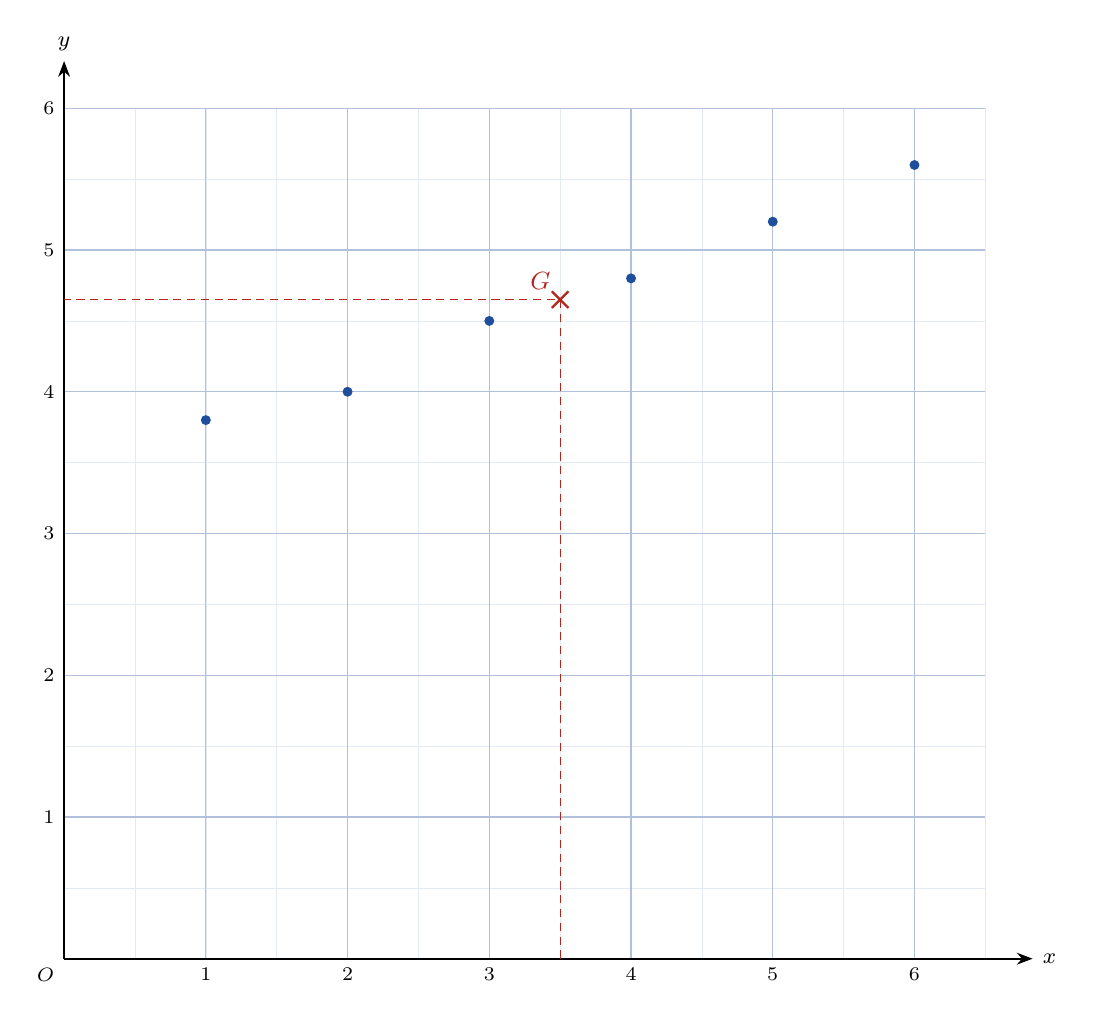
\begin{tikzpicture}[font=\footnotesize]
\draw[cDef!12,very thin](0.000,0)--(0.000,10.800);
\draw[cDef!12,very thin](0.900,0)--(0.900,10.800);
\draw[cDef!12,very thin](1.800,0)--(1.800,10.800);
\draw[cDef!12,very thin](2.700,0)--(2.700,10.800);
\draw[cDef!12,very thin](3.600,0)--(3.600,10.800);
\draw[cDef!12,very thin](4.500,0)--(4.500,10.800);
\draw[cDef!12,very thin](5.400,0)--(5.400,10.800);
\draw[cDef!12,very thin](6.300,0)--(6.300,10.800);
\draw[cDef!12,very thin](7.200,0)--(7.200,10.800);
\draw[cDef!12,very thin](8.100,0)--(8.100,10.800);
\draw[cDef!12,very thin](9.000,0)--(9.000,10.800);
\draw[cDef!12,very thin](9.900,0)--(9.900,10.800);
\draw[cDef!12,very thin](10.800,0)--(10.800,10.800);
\draw[cDef!12,very thin](11.700,0)--(11.700,10.800);
\draw[cDef!12,very thin](0,0.000)--(11.700,0.000);
\draw[cDef!12,very thin](0,0.900)--(11.700,0.900);
\draw[cDef!12,very thin](0,1.800)--(11.700,1.800);
\draw[cDef!12,very thin](0,2.700)--(11.700,2.700);
\draw[cDef!12,very thin](0,3.600)--(11.700,3.600);
\draw[cDef!12,very thin](0,4.500)--(11.700,4.500);
\draw[cDef!12,very thin](0,5.400)--(11.700,5.400);
\draw[cDef!12,very thin](0,6.300)--(11.700,6.300);
\draw[cDef!12,very thin](0,7.200)--(11.700,7.200);
\draw[cDef!12,very thin](0,8.100)--(11.700,8.100);
\draw[cDef!12,very thin](0,9.000)--(11.700,9.000);
\draw[cDef!12,very thin](0,9.900)--(11.700,9.900);
\draw[cDef!12,very thin](0,10.800)--(11.700,10.800);
\draw[cDef!35,thin](0.000,0)--(0.000,10.800);
\draw[cDef!35,thin](1.800,0)--(1.800,10.800);
\draw[cDef!35,thin](3.600,0)--(3.600,10.800);
\draw[cDef!35,thin](5.400,0)--(5.400,10.800);
\draw[cDef!35,thin](7.200,0)--(7.200,10.800);
\draw[cDef!35,thin](9.000,0)--(9.000,10.800);
\draw[cDef!35,thin](10.800,0)--(10.800,10.800);
\draw[cDef!35,thin](0,0.000)--(11.700,0.000);
\draw[cDef!35,thin](0,1.800)--(11.700,1.800);
\draw[cDef!35,thin](0,3.600)--(11.700,3.600);
\draw[cDef!35,thin](0,5.400)--(11.700,5.400);
\draw[cDef!35,thin](0,7.200)--(11.700,7.200);
\draw[cDef!35,thin](0,9.000)--(11.700,9.000);
\draw[cDef!35,thin](0,10.800)--(11.700,10.800);
\draw[-{Stealth[length=2mm]},thick](0,0)--(12.300,0) node[right]{$x$};
\draw[-{Stealth[length=2mm]},thick](0,0)--(0,11.400) node[above]{$y$};
\node[below,font=\scriptsize] at (1.800,0){$1$};
\node[below,font=\scriptsize] at (3.600,0){$2$};
\node[below,font=\scriptsize] at (5.400,0){$3$};
\node[below,font=\scriptsize] at (7.200,0){$4$};
\node[below,font=\scriptsize] at (9.000,0){$5$};
\node[below,font=\scriptsize] at (10.800,0){$6$};
\node[left,font=\scriptsize] at (0,1.800){$1$};
\node[left,font=\scriptsize] at (0,3.600){$2$};
\node[left,font=\scriptsize] at (0,5.400){$3$};
\node[left,font=\scriptsize] at (0,7.200){$4$};
\node[left,font=\scriptsize] at (0,9.000){$5$};
\node[left,font=\scriptsize] at (0,10.800){$6$};
\node[below left,font=\scriptsize] at (0,0){$O$};
\begin{scope}\clip(0,0) rectangle (11.700,10.800);
\end{scope}
\fill[cDef](1.800,6.840) circle (1.8pt);
\fill[cDef](3.600,7.200) circle (1.8pt);
\fill[cDef](5.400,8.100) circle (1.8pt);
\fill[cDef](7.200,8.640) circle (1.8pt);
\fill[cDef](9.000,9.360) circle (1.8pt);
\fill[cDef](10.800,10.080) circle (1.8pt);
\draw[cThm,densely dashed](6.300,0)--(6.300,8.370)--(0,8.370);
\draw[cThm,thick](6.300,8.370) +(-3pt,-3pt)--+(3pt,3pt) +(-3pt,3pt)--+(3pt,-3pt);
\node[cThm,above left,font=\small\bfseries] at (6.300,8.370){$G$};
\end{tikzpicture}\end{LTR}\end{center}

\QQ{2} النقطة المتوسطة $G(\bar x;\bar y)$ حيث:
\[\bar x=\frac{1+2+3+4+5+6}{6}=\frac{21}{6}=3{,}5\qquad \bar y=\frac{3{,}8+4+4{,}5+4{,}8+5{,}2+5{,}6}{6}=\frac{27{,}9}{6}=4{,}65\]
إذن \bx{G(3{,}5\,;\,4{,}65)}.

\QQ{3}
\pa جدول الحساب:
\begin{center}\begin{LTR}\renewcommand{\arraystretch}{1.25}
\begin{tabular}{|>{\columncolor{cSec!6}}c|*{6}{c|}>{\columncolor{cEx!10}}c|}\hline
\rowcolor{cSec!12}$x_i$ & 1 & 2 & 3 & 4 & 5 & 6 & $21$\\\hline
$y_i$ & $3{,}8$ & $4$ & $4{,}5$ & $4{,}8$ & $5{,}2$ & $5{,}6$ & $27{,}9$\\\hline
$x_i^2$ & 1 & 4 & 9 & 16 & 25 & 36 & $91$\\\hline
$x_iy_i$ & $3{,}8$ & $8$ & $13{,}5$ & $19{,}2$ & $26$ & $33{,}6$ & $104{,}1$\\\hline
\end{tabular}\end{LTR}\end{center}
\[V(x)=\frac{\sum x_i^2}{6}-\bar x^{2}=\frac{91}{6}-3{,}5^{2}\approx15{,}1667-12{,}25=2{,}9167\]
\[\operatorname{cov}(x,y)=\frac{\sum x_iy_i}{6}-\bar x\,\bar y=\frac{104{,}1}{6}-3{,}5\times4{,}65=17{,}35-16{,}275=1{,}075\]
\[a=\frac{\operatorname{cov}(x,y)}{V(x)}=\frac{1{,}075}{2{,}9167}\approx0{,}3686\ \Longrightarrow\ \bx{a\approx0{,}37}\]
$G\in(D)$ معناه $\bar y=a\bar x+b$ أي $b=\bar y-a\bar x=4{,}65-0{,}37\times3{,}5=4{,}65-1{,}295=3{,}355\approx3{,}36$.

\[\bx{(D):\ y=0{,}37x+3{,}36}\]
\pb سنة 2009 توافق الرتبة $x=10$:
\[y=0{,}37\times10+3{,}36=7{,}06\]
بما أن $7{,}06<7{,}3$ فإن \bxt{الهدف لا يتحقق حسب هذا التعديل} (الإنتاج المتوقع حوالي $7{,}06$ مليون طن).
\end{hal}

% ===================== بكالوريا 2008 -- الموضوع الثاني =====================
\begin{tamrin}{بكالوريا 2008 -- الموضوع الثاني -- تسيير واقتصاد}
الجدول التالي يمثل تطور نسبة البطالة في بلد بين السنوات 1970 و 2005.
\begin{center}\begin{LTR}\renewcommand{\arraystretch}{1.25}
\begin{tabular}{|>{\columncolor{cSec!6}}c|*{8}{c|}}\hline
\rowcolor{cSec!12}\ar{السنة $a_i$} & 1970 & 1975 & 1980 & 1985 & 1990 & 1995 & 2000 & 2005\\\hline
\ar{رتبة السنة $x_i=a_i-1970$} & 0 & 5 & 10 & 15 & 20 & 25 & 30 & 35\\\hline
\ar{النسبة المئوية $y_i$} & $1{,}3$ & $1{,}5$ & $1{,}5$ & $1{,}3$ & $1{,}4$ & $2{,}2$ & $2{,}5$ & $2$\\\hline
\end{tabular}\end{LTR}\end{center}
\QQ{1} مثّل بيانيا سحابة النقط $M_i(x_i;y_i)$ في معلم متعامد. ($1\,cm$ لكل 5 سنوات على محور الفواصل و $1\,cm$ لكل $0{,}5\%$ على محور التراتيب)
\QQ{2} جد إحداثيي النقطة المتوسطة $G$ لسحابة النقط ثم علّمها.
\QQ{3}
\begin{sq}
\qa بيّن أن المعادلة المختصرة لـ $(\Delta)$ مستقيم الانحدار بالمربعات الدنيا لهذه السلسلة هي: $y=0{,}03x+1{,}19$ ثم ارسمه.
\qb ما هي نسبة البطالة المتوقعة في هذا البلد سنة 2009؟
\qc ابتداء من أي سنة تصبح النسبة المتوقعة للبطالة أكبر من $3\%$؟
\end{sq}
\end{tamrin}

\Needspace{30\baselineskip}
\begin{hal}
\par\smallskip\textbf{1، 2 و 3(أ).}  سحابة النقط، النقطة $G$ والمستقيم $(\Delta)$:
\begin{center}\begin{LTR}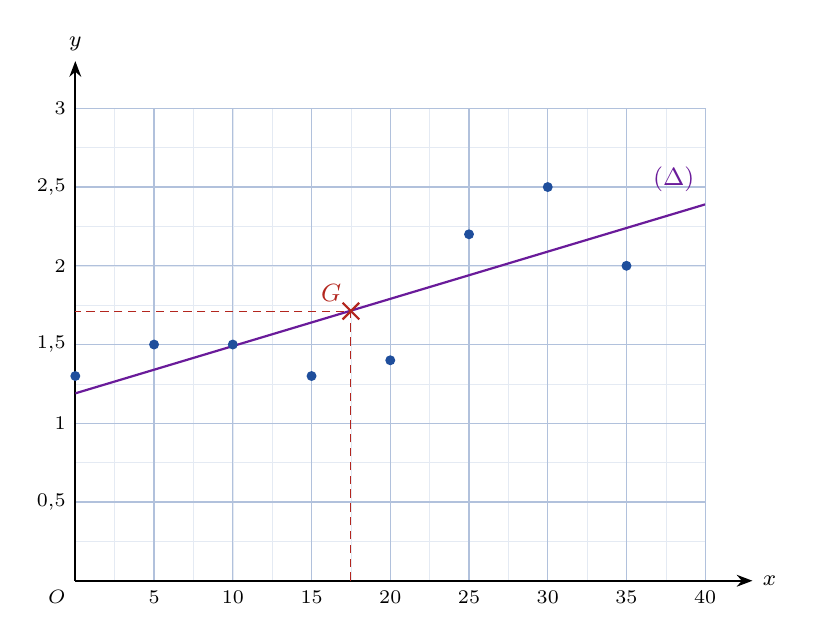
\begin{tikzpicture}[font=\footnotesize]
\draw[cDef!12,very thin](0.000,0)--(0.000,6.000);
\draw[cDef!12,very thin](0.500,0)--(0.500,6.000);
\draw[cDef!12,very thin](1.000,0)--(1.000,6.000);
\draw[cDef!12,very thin](1.500,0)--(1.500,6.000);
\draw[cDef!12,very thin](2.000,0)--(2.000,6.000);
\draw[cDef!12,very thin](2.500,0)--(2.500,6.000);
\draw[cDef!12,very thin](3.000,0)--(3.000,6.000);
\draw[cDef!12,very thin](3.500,0)--(3.500,6.000);
\draw[cDef!12,very thin](4.000,0)--(4.000,6.000);
\draw[cDef!12,very thin](4.500,0)--(4.500,6.000);
\draw[cDef!12,very thin](5.000,0)--(5.000,6.000);
\draw[cDef!12,very thin](5.500,0)--(5.500,6.000);
\draw[cDef!12,very thin](6.000,0)--(6.000,6.000);
\draw[cDef!12,very thin](6.500,0)--(6.500,6.000);
\draw[cDef!12,very thin](7.000,0)--(7.000,6.000);
\draw[cDef!12,very thin](7.500,0)--(7.500,6.000);
\draw[cDef!12,very thin](8.000,0)--(8.000,6.000);
\draw[cDef!12,very thin](0,0.000)--(8.000,0.000);
\draw[cDef!12,very thin](0,0.500)--(8.000,0.500);
\draw[cDef!12,very thin](0,1.000)--(8.000,1.000);
\draw[cDef!12,very thin](0,1.500)--(8.000,1.500);
\draw[cDef!12,very thin](0,2.000)--(8.000,2.000);
\draw[cDef!12,very thin](0,2.500)--(8.000,2.500);
\draw[cDef!12,very thin](0,3.000)--(8.000,3.000);
\draw[cDef!12,very thin](0,3.500)--(8.000,3.500);
\draw[cDef!12,very thin](0,4.000)--(8.000,4.000);
\draw[cDef!12,very thin](0,4.500)--(8.000,4.500);
\draw[cDef!12,very thin](0,5.000)--(8.000,5.000);
\draw[cDef!12,very thin](0,5.500)--(8.000,5.500);
\draw[cDef!12,very thin](0,6.000)--(8.000,6.000);
\draw[cDef!35,thin](0.000,0)--(0.000,6.000);
\draw[cDef!35,thin](1.000,0)--(1.000,6.000);
\draw[cDef!35,thin](2.000,0)--(2.000,6.000);
\draw[cDef!35,thin](3.000,0)--(3.000,6.000);
\draw[cDef!35,thin](4.000,0)--(4.000,6.000);
\draw[cDef!35,thin](5.000,0)--(5.000,6.000);
\draw[cDef!35,thin](6.000,0)--(6.000,6.000);
\draw[cDef!35,thin](7.000,0)--(7.000,6.000);
\draw[cDef!35,thin](8.000,0)--(8.000,6.000);
\draw[cDef!35,thin](0,0.000)--(8.000,0.000);
\draw[cDef!35,thin](0,1.000)--(8.000,1.000);
\draw[cDef!35,thin](0,2.000)--(8.000,2.000);
\draw[cDef!35,thin](0,3.000)--(8.000,3.000);
\draw[cDef!35,thin](0,4.000)--(8.000,4.000);
\draw[cDef!35,thin](0,5.000)--(8.000,5.000);
\draw[cDef!35,thin](0,6.000)--(8.000,6.000);
\draw[-{Stealth[length=2mm]},thick](0,0)--(8.600,0) node[right]{$x$};
\draw[-{Stealth[length=2mm]},thick](0,0)--(0,6.600) node[above]{$y$};
\node[below,font=\scriptsize] at (1.000,0){$5$};
\node[below,font=\scriptsize] at (2.000,0){$10$};
\node[below,font=\scriptsize] at (3.000,0){$15$};
\node[below,font=\scriptsize] at (4.000,0){$20$};
\node[below,font=\scriptsize] at (5.000,0){$25$};
\node[below,font=\scriptsize] at (6.000,0){$30$};
\node[below,font=\scriptsize] at (7.000,0){$35$};
\node[below,font=\scriptsize] at (8.000,0){$40$};
\node[left,font=\scriptsize] at (0,1.000){$0{,}5$};
\node[left,font=\scriptsize] at (0,2.000){$1$};
\node[left,font=\scriptsize] at (0,3.000){$1{,}5$};
\node[left,font=\scriptsize] at (0,4.000){$2$};
\node[left,font=\scriptsize] at (0,5.000){$2{,}5$};
\node[left,font=\scriptsize] at (0,6.000){$3$};
\node[below left,font=\scriptsize] at (0,0){$O$};
\begin{scope}\clip(0,0) rectangle (8.000,6.000);
\draw[cMeth,thick](0.000,2.380)--(8.000,4.780);
\end{scope}
\node[cMeth,font=\small] at (7.600,5.100){$(\Delta)$};
\fill[cDef](0.000,2.600) circle (1.8pt);
\fill[cDef](1.000,3.000) circle (1.8pt);
\fill[cDef](2.000,3.000) circle (1.8pt);
\fill[cDef](3.000,2.600) circle (1.8pt);
\fill[cDef](4.000,2.800) circle (1.8pt);
\fill[cDef](5.000,4.400) circle (1.8pt);
\fill[cDef](6.000,5.000) circle (1.8pt);
\fill[cDef](7.000,4.000) circle (1.8pt);
\draw[cThm,densely dashed](3.500,0)--(3.500,3.425)--(0,3.425);
\draw[cThm,thick](3.500,3.425) +(-3pt,-3pt)--+(3pt,3pt) +(-3pt,3pt)--+(3pt,-3pt);
\node[cThm,above left,font=\small\bfseries] at (3.500,3.425){$G$};
\end{tikzpicture}\end{LTR}\end{center}

\QQ{2} \[\bar x=\frac{0+5+10+15+20+25+30+35}{8}=\frac{140}{8}=17{,}5\qquad \bar y=\frac{13{,}7}{8}=1{,}7125\approx1{,}71\]
إذن \bx{G(17{,}5\,;\,1{,}71)} (مُعلَّمة بالأحمر في الشكل).

\QQ{3}
\pa جدول الحساب:
\begin{center}\begin{LTR}\renewcommand{\arraystretch}{1.25}\small
\begin{tabular}{|>{\columncolor{cSec!6}}c|*{8}{c|}>{\columncolor{cEx!10}}c|}\hline
\rowcolor{cSec!12}$x_i$ & 0 & 5 & 10 & 15 & 20 & 25 & 30 & 35 & $140$\\\hline
$y_i$ & $1{,}3$ & $1{,}5$ & $1{,}5$ & $1{,}3$ & $1{,}4$ & $2{,}2$ & $2{,}5$ & $2$ & $13{,}7$\\\hline
$x_i^2$ & 0 & 25 & 100 & 225 & 400 & 625 & 900 & 1225 & $3500$\\\hline
$x_iy_i$ & 0 & $7{,}5$ & $15$ & $19{,}5$ & $28$ & $55$ & $75$ & $70$ & $270$\\\hline
\end{tabular}\end{LTR}\end{center}
\[V(x)=\frac{3500}{8}-17{,}5^{2}=437{,}5-306{,}25=131{,}25\]
\[\operatorname{cov}(x,y)=\frac{270}{8}-17{,}5\times1{,}7125=33{,}75-29{,}96875=3{,}78125\]
\[a=\frac{3{,}78125}{131{,}25}\approx0{,}0288\approx0{,}03\]
\[b=\bar y-a\bar x=1{,}7125-0{,}03\times17{,}5=1{,}7125-0{,}525=1{,}1875\approx1{,}19\]
\[\bx{(\Delta):\ y=0{,}03x+1{,}19}\]
لرسمه: يشمل $G$ والنقطة $(0;1{,}19)$ (أو $(30;2{,}09)$).
\begin{molahada}
القيمة $b=1{,}19$ ناتجة عن تدوير $a$ إلى $0{,}03$ أولا. بالقيمة الدقيقة $a\approx0{,}0288$ نجد $b\approx1{,}21$. نعتمد معادلة النص.
\end{molahada}
\pb سنة 2009 توافق $x=2009-1970=39$:
\[y=0{,}03\times39+1{,}19=1{,}17+1{,}19=2{,}36\]
النسبة المتوقعة: \bx{2{,}36\,\%}.
\pc نحل $0{,}03x+1{,}19>3$ أي $0{,}03x>1{,}81$ أي $x>\dfrac{1{,}81}{0{,}03}\approx60{,}33$.

$x=a-1970>60{,}33$ يعني $a>2030{,}33$: \bxt{ابتداء من سنة 2031} تصبح النسبة أكبر من $3\%$.
\end{hal}

% ===================== بكالوريا 2009 -- الموضوع الثاني =====================
\begin{tamrin}{بكالوريا 2009 -- الموضوع الثاني -- تسيير واقتصاد}
يمثل الجدول التالي عدد الزوار (بالآلاف) لأحد الحمامات المعدنية بين سنتي 2000 و 2007.
\begin{center}\begin{LTR}\renewcommand{\arraystretch}{1.25}
\begin{tabular}{|>{\columncolor{cSec!6}}c|*{8}{c|}}\hline
\rowcolor{cSec!12}\ar{السنة} & 2000 & 2001 & 2002 & 2003 & 2004 & 2005 & 2006 & 2007\\\hline
\ar{رتبة السنة} & 1 & 2 & 3 & 4 & 5 & 6 & 7 & 8\\\hline
\ar{عدد الزوار $y_i$ (بالآلاف)} & $4{,}5$ & $4{,}9$ & $5{,}5$ & $5{,}2$ & $5{,}7$ & $6$ & $6{,}8$ & $7{,}4$\\\hline
\end{tabular}\end{LTR}\end{center}
\QQ{1} مثّل سحابة النقط المرفقة بالسلسلة الإحصائية $M_i(x_i;y_i)$ في معلم متعامد. (على محور الفواصل $2\,cm$ تمثل سنة واحدة، على محور التراتيب: $1\,cm$ ألف زائر)
\QQ{2} عيّن إحداثيي النقطة المتوسطة $G$ لهذه السلسلة ثم علّمها.
\QQ{3} بيّن أن المعادلة المختصرة لمستقيم الانحدار بالمربعات الدنيا لهذه السلسلة تكتب على الشكل: $y=0{,}38x+4$.
\QQ{4} باستعمال التعديل الخطي السابق عيّن عدد زوار هذا الحمام في سنة 2010.
\end{tamrin}

\Needspace{30\baselineskip}
\begin{hal}
\par\smallskip\textbf{1 و 2.}  سحابة النقط والنقطة $G$ (الرسم مصغّر قليلا):
\begin{center}\begin{LTR}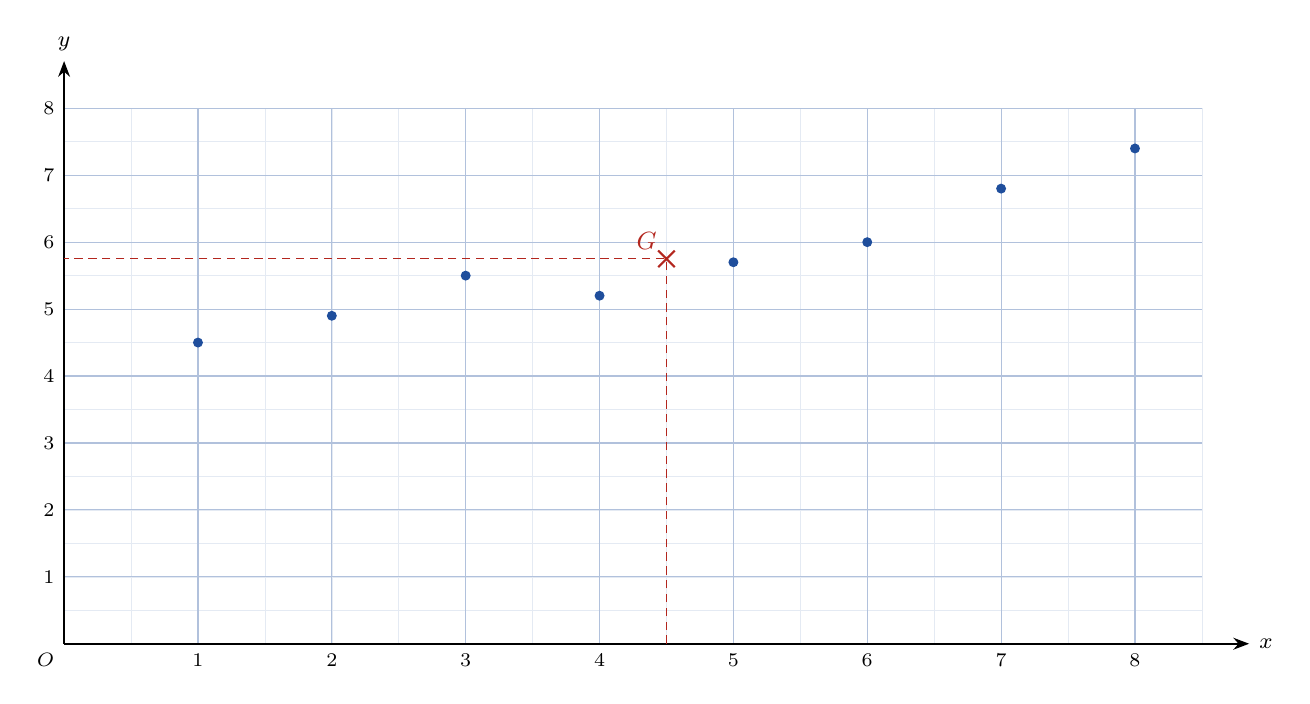
\begin{tikzpicture}[font=\footnotesize]
\draw[cDef!12,very thin](0.000,0)--(0.000,6.800);
\draw[cDef!12,very thin](0.850,0)--(0.850,6.800);
\draw[cDef!12,very thin](1.700,0)--(1.700,6.800);
\draw[cDef!12,very thin](2.550,0)--(2.550,6.800);
\draw[cDef!12,very thin](3.400,0)--(3.400,6.800);
\draw[cDef!12,very thin](4.250,0)--(4.250,6.800);
\draw[cDef!12,very thin](5.100,0)--(5.100,6.800);
\draw[cDef!12,very thin](5.950,0)--(5.950,6.800);
\draw[cDef!12,very thin](6.800,0)--(6.800,6.800);
\draw[cDef!12,very thin](7.650,0)--(7.650,6.800);
\draw[cDef!12,very thin](8.500,0)--(8.500,6.800);
\draw[cDef!12,very thin](9.350,0)--(9.350,6.800);
\draw[cDef!12,very thin](10.200,0)--(10.200,6.800);
\draw[cDef!12,very thin](11.050,0)--(11.050,6.800);
\draw[cDef!12,very thin](11.900,0)--(11.900,6.800);
\draw[cDef!12,very thin](12.750,0)--(12.750,6.800);
\draw[cDef!12,very thin](13.600,0)--(13.600,6.800);
\draw[cDef!12,very thin](14.450,0)--(14.450,6.800);
\draw[cDef!12,very thin](0,0.000)--(14.450,0.000);
\draw[cDef!12,very thin](0,0.425)--(14.450,0.425);
\draw[cDef!12,very thin](0,0.850)--(14.450,0.850);
\draw[cDef!12,very thin](0,1.275)--(14.450,1.275);
\draw[cDef!12,very thin](0,1.700)--(14.450,1.700);
\draw[cDef!12,very thin](0,2.125)--(14.450,2.125);
\draw[cDef!12,very thin](0,2.550)--(14.450,2.550);
\draw[cDef!12,very thin](0,2.975)--(14.450,2.975);
\draw[cDef!12,very thin](0,3.400)--(14.450,3.400);
\draw[cDef!12,very thin](0,3.825)--(14.450,3.825);
\draw[cDef!12,very thin](0,4.250)--(14.450,4.250);
\draw[cDef!12,very thin](0,4.675)--(14.450,4.675);
\draw[cDef!12,very thin](0,5.100)--(14.450,5.100);
\draw[cDef!12,very thin](0,5.525)--(14.450,5.525);
\draw[cDef!12,very thin](0,5.950)--(14.450,5.950);
\draw[cDef!12,very thin](0,6.375)--(14.450,6.375);
\draw[cDef!12,very thin](0,6.800)--(14.450,6.800);
\draw[cDef!35,thin](0.000,0)--(0.000,6.800);
\draw[cDef!35,thin](1.700,0)--(1.700,6.800);
\draw[cDef!35,thin](3.400,0)--(3.400,6.800);
\draw[cDef!35,thin](5.100,0)--(5.100,6.800);
\draw[cDef!35,thin](6.800,0)--(6.800,6.800);
\draw[cDef!35,thin](8.500,0)--(8.500,6.800);
\draw[cDef!35,thin](10.200,0)--(10.200,6.800);
\draw[cDef!35,thin](11.900,0)--(11.900,6.800);
\draw[cDef!35,thin](13.600,0)--(13.600,6.800);
\draw[cDef!35,thin](0,0.000)--(14.450,0.000);
\draw[cDef!35,thin](0,0.850)--(14.450,0.850);
\draw[cDef!35,thin](0,1.700)--(14.450,1.700);
\draw[cDef!35,thin](0,2.550)--(14.450,2.550);
\draw[cDef!35,thin](0,3.400)--(14.450,3.400);
\draw[cDef!35,thin](0,4.250)--(14.450,4.250);
\draw[cDef!35,thin](0,5.100)--(14.450,5.100);
\draw[cDef!35,thin](0,5.950)--(14.450,5.950);
\draw[cDef!35,thin](0,6.800)--(14.450,6.800);
\draw[-{Stealth[length=2mm]},thick](0,0)--(15.050,0) node[right]{$x$};
\draw[-{Stealth[length=2mm]},thick](0,0)--(0,7.400) node[above]{$y$};
\node[below,font=\scriptsize] at (1.700,0){$1$};
\node[below,font=\scriptsize] at (3.400,0){$2$};
\node[below,font=\scriptsize] at (5.100,0){$3$};
\node[below,font=\scriptsize] at (6.800,0){$4$};
\node[below,font=\scriptsize] at (8.500,0){$5$};
\node[below,font=\scriptsize] at (10.200,0){$6$};
\node[below,font=\scriptsize] at (11.900,0){$7$};
\node[below,font=\scriptsize] at (13.600,0){$8$};
\node[left,font=\scriptsize] at (0,0.850){$1$};
\node[left,font=\scriptsize] at (0,1.700){$2$};
\node[left,font=\scriptsize] at (0,2.550){$3$};
\node[left,font=\scriptsize] at (0,3.400){$4$};
\node[left,font=\scriptsize] at (0,4.250){$5$};
\node[left,font=\scriptsize] at (0,5.100){$6$};
\node[left,font=\scriptsize] at (0,5.950){$7$};
\node[left,font=\scriptsize] at (0,6.800){$8$};
\node[below left,font=\scriptsize] at (0,0){$O$};
\begin{scope}\clip(0,0) rectangle (14.450,6.800);
\end{scope}
\fill[cDef](1.700,3.825) circle (1.8pt);
\fill[cDef](3.400,4.165) circle (1.8pt);
\fill[cDef](5.100,4.675) circle (1.8pt);
\fill[cDef](6.800,4.420) circle (1.8pt);
\fill[cDef](8.500,4.845) circle (1.8pt);
\fill[cDef](10.200,5.100) circle (1.8pt);
\fill[cDef](11.900,5.780) circle (1.8pt);
\fill[cDef](13.600,6.290) circle (1.8pt);
\draw[cThm,densely dashed](7.650,0)--(7.650,4.888)--(0,4.888);
\draw[cThm,thick](7.650,4.888) +(-3pt,-3pt)--+(3pt,3pt) +(-3pt,3pt)--+(3pt,-3pt);
\node[cThm,above left,font=\small\bfseries] at (7.650,4.888){$G$};
\end{tikzpicture}\end{LTR}\end{center}
\[\bar x=\frac{36}{8}=4{,}5\qquad \bar y=\frac{46}{8}=5{,}75\qquad \bx{G(4{,}5\,;\,5{,}75)}\]

\QQ{3} جدول الحساب:
\begin{center}\begin{LTR}\renewcommand{\arraystretch}{1.25}
\begin{tabular}{|>{\columncolor{cSec!6}}c|*{8}{c|}>{\columncolor{cEx!10}}c|}\hline
\rowcolor{cSec!12}$x_i$ & 1 & 2 & 3 & 4 & 5 & 6 & 7 & 8 & $36$\\\hline
$y_i$ & $4{,}5$ & $4{,}9$ & $5{,}5$ & $5{,}2$ & $5{,}7$ & $6$ & $6{,}8$ & $7{,}4$ & $46$\\\hline
$x_i^2$ & 1 & 4 & 9 & 16 & 25 & 36 & 49 & 64 & $204$\\\hline
$x_iy_i$ & $4{,}5$ & $9{,}8$ & $16{,}5$ & $20{,}8$ & $28{,}5$ & $36$ & $47{,}6$ & $59{,}2$ & $222{,}9$\\\hline
\end{tabular}\end{LTR}\end{center}
\[V(x)=\frac{204}{8}-4{,}5^{2}=25{,}5-20{,}25=5{,}25\]
\[\operatorname{cov}(x,y)=\frac{222{,}9}{8}-4{,}5\times5{,}75=27{,}8625-25{,}875=1{,}9875\]
\[a=\frac{1{,}9875}{5{,}25}\approx0{,}3786\approx0{,}38\]
\[b=\bar y-a\bar x=5{,}75-0{,}38\times4{,}5=5{,}75-1{,}71=4{,}04\approx4\]
\[\bx{y=0{,}38x+4}\]
\begin{molahada}
الحساب يعطي $b\approx4{,}04$ ؛ النص دوّر $b$ إلى الوحدة فكتب $y=0{,}38x+4$. نعتمد معادلة النص.
\end{molahada}

\QQ{4} سنة 2010 توافق الرتبة $x=11$:
\[y=0{,}38\times11+4=4{,}18+4=8{,}18\]
عدد الزوار المتوقع سنة 2010: \bxt{حوالي $8180$ زائرا}.
\end{hal}

% ===================== بكالوريا 2010 -- الموضوع الأول =====================
\begin{tamrin}{بكالوريا 2010 -- الموضوع الأول -- تسيير واقتصاد}
يمثل الجدول التالي ضغط الدم $y_i$ بدلالة السن $x_i$ لعينة من الرجال.
\begin{center}\begin{LTR}\renewcommand{\arraystretch}{1.25}
\begin{tabular}{|>{\columncolor{cSec!6}}c|*{7}{c|}}\hline
\rowcolor{cSec!12}\ar{السن $x_i$} & 35 & 40 & 45 & 50 & 55 & 60 & 65\\\hline
\ar{ضغط الدم $y_i$} & $12{,}2$ & $12{,}4$ & $12{,}5$ & $13$ & $13{,}3$ & $13{,}6$ & $14$\\\hline
\end{tabular}\end{LTR}\end{center}
\QQ{1} مثّل بسحابة نقط $M_i(x_i;y_i)$ في معلم متعامد مبدؤه $O'(30;11)$ وبوحدة $1\,cm$ لكل 5 سنوات على محور الفواصل و $2\,cm$ لكل وحدة على محور التراتيب.
\QQ{2}
\begin{sq}
\qa عيّن إحداثيي $G$ النقطة المتوسطة للسحابة.
\qb مثّل النقطة $G$ في المعلم السابق.
\end{sq}
\QQ{3} أوجد معادلة مستقيم الانحدار بالمربعات الدنيا: $y=ax+b$، تعطى $a$ و $b$ مدوّرة إلى $10^{-2}$. ارسم هذا المستقيم في المعلم السابق.
\QQ{4} رجل عمره 70 سنة وضغط دمه $15{,}2$. هل هذا معقول حسب هذا التعديل؟ علّل.
\end{tamrin}

\Needspace{30\baselineskip}
\begin{hal}
\par\smallskip\textbf{1، 2(ب) و 3.}  السحابة، $G$ والمستقيم $(D)$، مع النقطة $M(70;15{,}2)$ للسؤال 4:
\begin{center}\begin{LTR}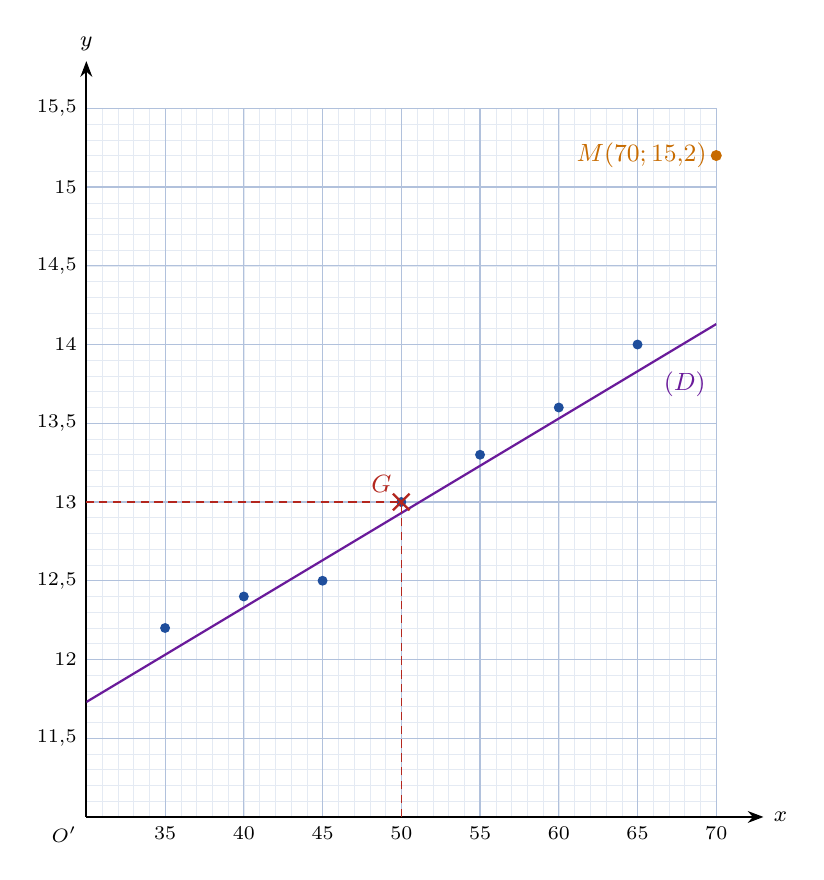
\begin{tikzpicture}[font=\footnotesize]
\draw[cDef!12,very thin](0.000,0)--(0.000,9.000);
\draw[cDef!12,very thin](0.200,0)--(0.200,9.000);
\draw[cDef!12,very thin](0.400,0)--(0.400,9.000);
\draw[cDef!12,very thin](0.600,0)--(0.600,9.000);
\draw[cDef!12,very thin](0.800,0)--(0.800,9.000);
\draw[cDef!12,very thin](1.000,0)--(1.000,9.000);
\draw[cDef!12,very thin](1.200,0)--(1.200,9.000);
\draw[cDef!12,very thin](1.400,0)--(1.400,9.000);
\draw[cDef!12,very thin](1.600,0)--(1.600,9.000);
\draw[cDef!12,very thin](1.800,0)--(1.800,9.000);
\draw[cDef!12,very thin](2.000,0)--(2.000,9.000);
\draw[cDef!12,very thin](2.200,0)--(2.200,9.000);
\draw[cDef!12,very thin](2.400,0)--(2.400,9.000);
\draw[cDef!12,very thin](2.600,0)--(2.600,9.000);
\draw[cDef!12,very thin](2.800,0)--(2.800,9.000);
\draw[cDef!12,very thin](3.000,0)--(3.000,9.000);
\draw[cDef!12,very thin](3.200,0)--(3.200,9.000);
\draw[cDef!12,very thin](3.400,0)--(3.400,9.000);
\draw[cDef!12,very thin](3.600,0)--(3.600,9.000);
\draw[cDef!12,very thin](3.800,0)--(3.800,9.000);
\draw[cDef!12,very thin](4.000,0)--(4.000,9.000);
\draw[cDef!12,very thin](4.200,0)--(4.200,9.000);
\draw[cDef!12,very thin](4.400,0)--(4.400,9.000);
\draw[cDef!12,very thin](4.600,0)--(4.600,9.000);
\draw[cDef!12,very thin](4.800,0)--(4.800,9.000);
\draw[cDef!12,very thin](5.000,0)--(5.000,9.000);
\draw[cDef!12,very thin](5.200,0)--(5.200,9.000);
\draw[cDef!12,very thin](5.400,0)--(5.400,9.000);
\draw[cDef!12,very thin](5.600,0)--(5.600,9.000);
\draw[cDef!12,very thin](5.800,0)--(5.800,9.000);
\draw[cDef!12,very thin](6.000,0)--(6.000,9.000);
\draw[cDef!12,very thin](6.200,0)--(6.200,9.000);
\draw[cDef!12,very thin](6.400,0)--(6.400,9.000);
\draw[cDef!12,very thin](6.600,0)--(6.600,9.000);
\draw[cDef!12,very thin](6.800,0)--(6.800,9.000);
\draw[cDef!12,very thin](7.000,0)--(7.000,9.000);
\draw[cDef!12,very thin](7.200,0)--(7.200,9.000);
\draw[cDef!12,very thin](7.400,0)--(7.400,9.000);
\draw[cDef!12,very thin](7.600,0)--(7.600,9.000);
\draw[cDef!12,very thin](7.800,0)--(7.800,9.000);
\draw[cDef!12,very thin](8.000,0)--(8.000,9.000);
\draw[cDef!12,very thin](0,0.000)--(8.000,0.000);
\draw[cDef!12,very thin](0,0.200)--(8.000,0.200);
\draw[cDef!12,very thin](0,0.400)--(8.000,0.400);
\draw[cDef!12,very thin](0,0.600)--(8.000,0.600);
\draw[cDef!12,very thin](0,0.800)--(8.000,0.800);
\draw[cDef!12,very thin](0,1.000)--(8.000,1.000);
\draw[cDef!12,very thin](0,1.200)--(8.000,1.200);
\draw[cDef!12,very thin](0,1.400)--(8.000,1.400);
\draw[cDef!12,very thin](0,1.600)--(8.000,1.600);
\draw[cDef!12,very thin](0,1.800)--(8.000,1.800);
\draw[cDef!12,very thin](0,2.000)--(8.000,2.000);
\draw[cDef!12,very thin](0,2.200)--(8.000,2.200);
\draw[cDef!12,very thin](0,2.400)--(8.000,2.400);
\draw[cDef!12,very thin](0,2.600)--(8.000,2.600);
\draw[cDef!12,very thin](0,2.800)--(8.000,2.800);
\draw[cDef!12,very thin](0,3.000)--(8.000,3.000);
\draw[cDef!12,very thin](0,3.200)--(8.000,3.200);
\draw[cDef!12,very thin](0,3.400)--(8.000,3.400);
\draw[cDef!12,very thin](0,3.600)--(8.000,3.600);
\draw[cDef!12,very thin](0,3.800)--(8.000,3.800);
\draw[cDef!12,very thin](0,4.000)--(8.000,4.000);
\draw[cDef!12,very thin](0,4.200)--(8.000,4.200);
\draw[cDef!12,very thin](0,4.400)--(8.000,4.400);
\draw[cDef!12,very thin](0,4.600)--(8.000,4.600);
\draw[cDef!12,very thin](0,4.800)--(8.000,4.800);
\draw[cDef!12,very thin](0,5.000)--(8.000,5.000);
\draw[cDef!12,very thin](0,5.200)--(8.000,5.200);
\draw[cDef!12,very thin](0,5.400)--(8.000,5.400);
\draw[cDef!12,very thin](0,5.600)--(8.000,5.600);
\draw[cDef!12,very thin](0,5.800)--(8.000,5.800);
\draw[cDef!12,very thin](0,6.000)--(8.000,6.000);
\draw[cDef!12,very thin](0,6.200)--(8.000,6.200);
\draw[cDef!12,very thin](0,6.400)--(8.000,6.400);
\draw[cDef!12,very thin](0,6.600)--(8.000,6.600);
\draw[cDef!12,very thin](0,6.800)--(8.000,6.800);
\draw[cDef!12,very thin](0,7.000)--(8.000,7.000);
\draw[cDef!12,very thin](0,7.200)--(8.000,7.200);
\draw[cDef!12,very thin](0,7.400)--(8.000,7.400);
\draw[cDef!12,very thin](0,7.600)--(8.000,7.600);
\draw[cDef!12,very thin](0,7.800)--(8.000,7.800);
\draw[cDef!12,very thin](0,8.000)--(8.000,8.000);
\draw[cDef!12,very thin](0,8.200)--(8.000,8.200);
\draw[cDef!12,very thin](0,8.400)--(8.000,8.400);
\draw[cDef!12,very thin](0,8.600)--(8.000,8.600);
\draw[cDef!12,very thin](0,8.800)--(8.000,8.800);
\draw[cDef!12,very thin](0,9.000)--(8.000,9.000);
\draw[cDef!35,thin](0.000,0)--(0.000,9.000);
\draw[cDef!35,thin](1.000,0)--(1.000,9.000);
\draw[cDef!35,thin](2.000,0)--(2.000,9.000);
\draw[cDef!35,thin](3.000,0)--(3.000,9.000);
\draw[cDef!35,thin](4.000,0)--(4.000,9.000);
\draw[cDef!35,thin](5.000,0)--(5.000,9.000);
\draw[cDef!35,thin](6.000,0)--(6.000,9.000);
\draw[cDef!35,thin](7.000,0)--(7.000,9.000);
\draw[cDef!35,thin](8.000,0)--(8.000,9.000);
\draw[cDef!35,thin](0,0.000)--(8.000,0.000);
\draw[cDef!35,thin](0,1.000)--(8.000,1.000);
\draw[cDef!35,thin](0,2.000)--(8.000,2.000);
\draw[cDef!35,thin](0,3.000)--(8.000,3.000);
\draw[cDef!35,thin](0,4.000)--(8.000,4.000);
\draw[cDef!35,thin](0,5.000)--(8.000,5.000);
\draw[cDef!35,thin](0,6.000)--(8.000,6.000);
\draw[cDef!35,thin](0,7.000)--(8.000,7.000);
\draw[cDef!35,thin](0,8.000)--(8.000,8.000);
\draw[cDef!35,thin](0,9.000)--(8.000,9.000);
\draw[-{Stealth[length=2mm]},thick](0,0)--(8.600,0) node[right]{$x$};
\draw[-{Stealth[length=2mm]},thick](0,0)--(0,9.600) node[above]{$y$};
\node[below,font=\scriptsize] at (1.000,0){$35$};
\node[below,font=\scriptsize] at (2.000,0){$40$};
\node[below,font=\scriptsize] at (3.000,0){$45$};
\node[below,font=\scriptsize] at (4.000,0){$50$};
\node[below,font=\scriptsize] at (5.000,0){$55$};
\node[below,font=\scriptsize] at (6.000,0){$60$};
\node[below,font=\scriptsize] at (7.000,0){$65$};
\node[below,font=\scriptsize] at (8.000,0){$70$};
\node[left,font=\scriptsize] at (0,1.000){$11{,}5$};
\node[left,font=\scriptsize] at (0,2.000){$12$};
\node[left,font=\scriptsize] at (0,3.000){$12{,}5$};
\node[left,font=\scriptsize] at (0,4.000){$13$};
\node[left,font=\scriptsize] at (0,5.000){$13{,}5$};
\node[left,font=\scriptsize] at (0,6.000){$14$};
\node[left,font=\scriptsize] at (0,7.000){$14{,}5$};
\node[left,font=\scriptsize] at (0,8.000){$15$};
\node[left,font=\scriptsize] at (0,9.000){$15{,}5$};
\node[below left,font=\scriptsize] at (0,0){$O'$};
\begin{scope}\clip(0,0) rectangle (8.000,9.000);
\draw[cMeth,thick](0.000,1.460)--(8.000,6.260);
\end{scope}
\node[cMeth,font=\small] at (7.600,5.500){$(D)$};
\fill[cDef](1.000,2.400) circle (1.8pt);
\fill[cDef](2.000,2.800) circle (1.8pt);
\fill[cDef](3.000,3.000) circle (1.8pt);
\fill[cDef](4.000,4.000) circle (1.8pt);
\fill[cDef](5.000,4.600) circle (1.8pt);
\fill[cDef](6.000,5.200) circle (1.8pt);
\fill[cDef](7.000,6.000) circle (1.8pt);
\fill[cEx](8.000,8.400) circle (2pt) node[left,font=\small]{$M(70;15{,}2)$};
\draw[cThm,densely dashed](4.000,0)--(4.000,4.000)--(0,4.000);
\draw[cThm,thick](4.000,4.000) +(-3pt,-3pt)--+(3pt,3pt) +(-3pt,3pt)--+(3pt,-3pt);
\node[cThm,above left,font=\small\bfseries] at (4.000,4.000){$G$};
\end{tikzpicture}\end{LTR}\end{center}

\QQ{2}
\pa \[\bar x=\frac{350}{7}=50\qquad \bar y=\frac{91}{7}=13\qquad \bx{G(50\,;\,13)}\]

\QQ{3} جدول الحساب:
\begin{center}\begin{LTR}\renewcommand{\arraystretch}{1.25}
\begin{tabular}{|>{\columncolor{cSec!6}}c|*{7}{c|}>{\columncolor{cEx!10}}c|}\hline
\rowcolor{cSec!12}$x_i$ & 35 & 40 & 45 & 50 & 55 & 60 & 65 & $350$\\\hline
$y_i$ & $12{,}2$ & $12{,}4$ & $12{,}5$ & $13$ & $13{,}3$ & $13{,}6$ & $14$ & $91$\\\hline
$x_i^2$ & 1225 & 1600 & 2025 & 2500 & 3025 & 3600 & 4225 & $18200$\\\hline
$x_iy_i$ & $427$ & $496$ & $562{,}5$ & $650$ & $731{,}5$ & $816$ & $910$ & $4593$\\\hline
\end{tabular}\end{LTR}\end{center}
\[V(x)=\frac{18200}{7}-50^{2}=2600-2500=100\]
\[\operatorname{cov}(x,y)=\frac{4593}{7}-50\times13\approx656{,}1429-650=6{,}1429\]
\[a=\frac{6{,}1429}{100}\approx0{,}0614\approx0{,}06\]
\[b=\bar y-a\bar x=13-0{,}061429\times50\approx13-3{,}0714=9{,}9286\approx9{,}93\]
\[\bx{(D):\ y=0{,}06x+9{,}93}\]
لرسمه: يشمل $G(50;13)$ والنقطة $(30;11{,}73)$ أو $(70;14{,}13)$.

\QQ{4} حسب التعديل، رجل عمره 70 سنة:
\[y=0{,}06\times70+9{,}93=4{,}2+9{,}93=14{,}13\]
الضغط المقدّر $14{,}13$ بينما ضغط الرجل $15{,}2$، والفرق $15{,}2-14{,}13\approx1{,}07$ كبير (أكبر من الفرق بين أكبر وأصغر قيمة في الجدول تقريبا)؛ والنقطة $M(70;15{,}2)$ بعيدة عن المستقيم $(D)$ في الشكل.
إذن \bxt{هذا غير معقول حسب هذا التعديل} (ضغط الرجل أعلى من المتوقع).
\end{hal}

% ===================== بكالوريا 2010 -- الموضوع الثاني =====================
\begin{tamrin}{بكالوريا 2010 -- الموضوع الثاني -- تسيير واقتصاد}
يمثل الجدول التالي تطور إنتاج سنوي بالطن لأحد أنواع الأسماك في إحدى المجمعات المائية لتربية الأسماك:
\begin{center}\begin{LTR}\renewcommand{\arraystretch}{1.25}
\begin{tabular}{|>{\columncolor{cSec!6}}c|*{6}{c|}}\hline
\rowcolor{cSec!12}\ar{السنة} & 2004 & 2005 & 2006 & 2007 & 2008 & 2009\\\hline
\ar{ترتيب السنوات $x_i$} & 1 & 2 & 3 & 4 & 5 & 6\\\hline
\ar{الإنتاج $y_i$} & 530 & 640 & 770 & 850 & 980 & 1115\\\hline
\end{tabular}\end{LTR}\end{center}
\QQ{1} مثّل سحابة النقط $M_i(x_i;y_i)$ المرفقة بالسلسلة الإحصائية في معلم متعامد. (على محور الفواصل $2\,cm$ تمثل سنة واحدة، وعلى محور التراتيب $1\,cm$ يمثل 100 طن من السمك)
\QQ{2} عيّن إحداثيي النقطة المتوسطة $G$ لهذه السحابة.
\QQ{3} بيّن أن معادلة مستقيم الانحدار بالمربعات الدنيا هي: $y=115x+411{,}67$.
\QQ{4} عيّن إنتاج هذا المجمع المائي في سنة 2015. (تعطى كل النتائج مدوّرة إلى $10^{-2}$)
\end{tamrin}

\Needspace{30\baselineskip}
\begin{hal}
\QQ{1} سحابة النقط (الرسم مصغّر قليلا):
\begin{center}\begin{LTR}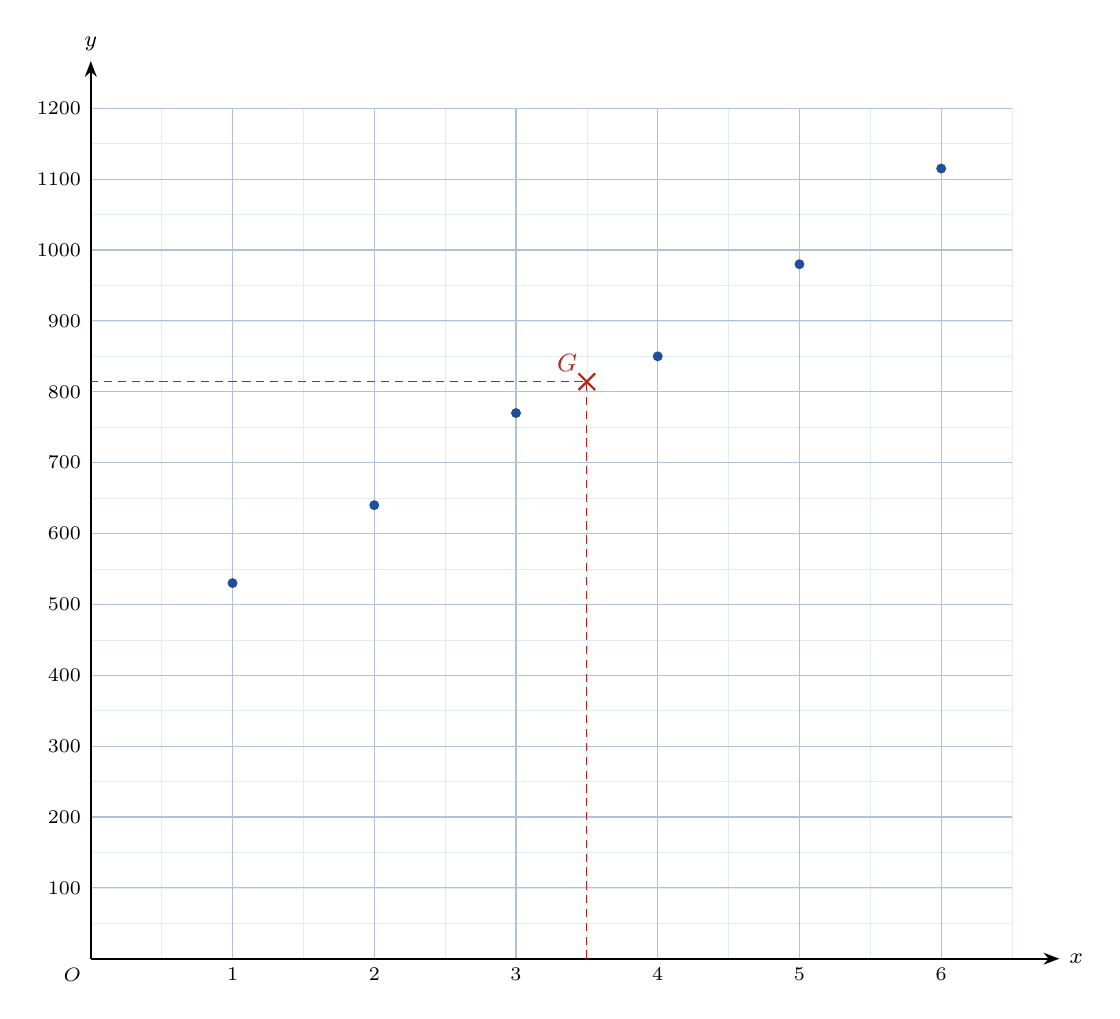
\begin{tikzpicture}[font=\footnotesize]
\draw[cDef!12,very thin](0.000,0)--(0.000,10.800);
\draw[cDef!12,very thin](0.900,0)--(0.900,10.800);
\draw[cDef!12,very thin](1.800,0)--(1.800,10.800);
\draw[cDef!12,very thin](2.700,0)--(2.700,10.800);
\draw[cDef!12,very thin](3.600,0)--(3.600,10.800);
\draw[cDef!12,very thin](4.500,0)--(4.500,10.800);
\draw[cDef!12,very thin](5.400,0)--(5.400,10.800);
\draw[cDef!12,very thin](6.300,0)--(6.300,10.800);
\draw[cDef!12,very thin](7.200,0)--(7.200,10.800);
\draw[cDef!12,very thin](8.100,0)--(8.100,10.800);
\draw[cDef!12,very thin](9.000,0)--(9.000,10.800);
\draw[cDef!12,very thin](9.900,0)--(9.900,10.800);
\draw[cDef!12,very thin](10.800,0)--(10.800,10.800);
\draw[cDef!12,very thin](11.700,0)--(11.700,10.800);
\draw[cDef!12,very thin](0,0.000)--(11.700,0.000);
\draw[cDef!12,very thin](0,0.450)--(11.700,0.450);
\draw[cDef!12,very thin](0,0.900)--(11.700,0.900);
\draw[cDef!12,very thin](0,1.350)--(11.700,1.350);
\draw[cDef!12,very thin](0,1.800)--(11.700,1.800);
\draw[cDef!12,very thin](0,2.250)--(11.700,2.250);
\draw[cDef!12,very thin](0,2.700)--(11.700,2.700);
\draw[cDef!12,very thin](0,3.150)--(11.700,3.150);
\draw[cDef!12,very thin](0,3.600)--(11.700,3.600);
\draw[cDef!12,very thin](0,4.050)--(11.700,4.050);
\draw[cDef!12,very thin](0,4.500)--(11.700,4.500);
\draw[cDef!12,very thin](0,4.950)--(11.700,4.950);
\draw[cDef!12,very thin](0,5.400)--(11.700,5.400);
\draw[cDef!12,very thin](0,5.850)--(11.700,5.850);
\draw[cDef!12,very thin](0,6.300)--(11.700,6.300);
\draw[cDef!12,very thin](0,6.750)--(11.700,6.750);
\draw[cDef!12,very thin](0,7.200)--(11.700,7.200);
\draw[cDef!12,very thin](0,7.650)--(11.700,7.650);
\draw[cDef!12,very thin](0,8.100)--(11.700,8.100);
\draw[cDef!12,very thin](0,8.550)--(11.700,8.550);
\draw[cDef!12,very thin](0,9.000)--(11.700,9.000);
\draw[cDef!12,very thin](0,9.450)--(11.700,9.450);
\draw[cDef!12,very thin](0,9.900)--(11.700,9.900);
\draw[cDef!12,very thin](0,10.350)--(11.700,10.350);
\draw[cDef!12,very thin](0,10.800)--(11.700,10.800);
\draw[cDef!35,thin](0.000,0)--(0.000,10.800);
\draw[cDef!35,thin](1.800,0)--(1.800,10.800);
\draw[cDef!35,thin](3.600,0)--(3.600,10.800);
\draw[cDef!35,thin](5.400,0)--(5.400,10.800);
\draw[cDef!35,thin](7.200,0)--(7.200,10.800);
\draw[cDef!35,thin](9.000,0)--(9.000,10.800);
\draw[cDef!35,thin](10.800,0)--(10.800,10.800);
\draw[cDef!35,thin](0,0.000)--(11.700,0.000);
\draw[cDef!35,thin](0,0.900)--(11.700,0.900);
\draw[cDef!35,thin](0,1.800)--(11.700,1.800);
\draw[cDef!35,thin](0,2.700)--(11.700,2.700);
\draw[cDef!35,thin](0,3.600)--(11.700,3.600);
\draw[cDef!35,thin](0,4.500)--(11.700,4.500);
\draw[cDef!35,thin](0,5.400)--(11.700,5.400);
\draw[cDef!35,thin](0,6.300)--(11.700,6.300);
\draw[cDef!35,thin](0,7.200)--(11.700,7.200);
\draw[cDef!35,thin](0,8.100)--(11.700,8.100);
\draw[cDef!35,thin](0,9.000)--(11.700,9.000);
\draw[cDef!35,thin](0,9.900)--(11.700,9.900);
\draw[cDef!35,thin](0,10.800)--(11.700,10.800);
\draw[-{Stealth[length=2mm]},thick](0,0)--(12.300,0) node[right]{$x$};
\draw[-{Stealth[length=2mm]},thick](0,0)--(0,11.400) node[above]{$y$};
\node[below,font=\scriptsize] at (1.800,0){$1$};
\node[below,font=\scriptsize] at (3.600,0){$2$};
\node[below,font=\scriptsize] at (5.400,0){$3$};
\node[below,font=\scriptsize] at (7.200,0){$4$};
\node[below,font=\scriptsize] at (9.000,0){$5$};
\node[below,font=\scriptsize] at (10.800,0){$6$};
\node[left,font=\scriptsize] at (0,0.900){$100$};
\node[left,font=\scriptsize] at (0,1.800){$200$};
\node[left,font=\scriptsize] at (0,2.700){$300$};
\node[left,font=\scriptsize] at (0,3.600){$400$};
\node[left,font=\scriptsize] at (0,4.500){$500$};
\node[left,font=\scriptsize] at (0,5.400){$600$};
\node[left,font=\scriptsize] at (0,6.300){$700$};
\node[left,font=\scriptsize] at (0,7.200){$800$};
\node[left,font=\scriptsize] at (0,8.100){$900$};
\node[left,font=\scriptsize] at (0,9.000){$1000$};
\node[left,font=\scriptsize] at (0,9.900){$1100$};
\node[left,font=\scriptsize] at (0,10.800){$1200$};
\node[below left,font=\scriptsize] at (0,0){$O$};
\begin{scope}\clip(0,0) rectangle (11.700,10.800);
\end{scope}
\fill[cDef](1.800,4.770) circle (1.8pt);
\fill[cDef](3.600,5.760) circle (1.8pt);
\fill[cDef](5.400,6.930) circle (1.8pt);
\fill[cDef](7.200,7.650) circle (1.8pt);
\fill[cDef](9.000,8.820) circle (1.8pt);
\fill[cDef](10.800,10.035) circle (1.8pt);
\draw[cThm,densely dashed](6.300,0)--(6.300,7.328)--(0,7.328);
\draw[cThm,thick](6.300,7.328) +(-3pt,-3pt)--+(3pt,3pt) +(-3pt,3pt)--+(3pt,-3pt);
\node[cThm,above left,font=\small\bfseries] at (6.300,7.328){$G$};
\end{tikzpicture}\end{LTR}\end{center}

\QQ{2} \[\bar x=\frac{21}{6}=3{,}5\qquad \bar y=\frac{4885}{6}\approx814{,}17\qquad \bx{G(3{,}5\,;\,814{,}17)}\]

\QQ{3} جدول الحساب:
\begin{center}\begin{LTR}\renewcommand{\arraystretch}{1.25}
\begin{tabular}{|>{\columncolor{cSec!6}}c|*{6}{c|}>{\columncolor{cEx!10}}c|}\hline
\rowcolor{cSec!12}$x_i$ & 1 & 2 & 3 & 4 & 5 & 6 & $21$\\\hline
$y_i$ & 530 & 640 & 770 & 850 & 980 & 1115 & $4885$\\\hline
$x_i^2$ & 1 & 4 & 9 & 16 & 25 & 36 & $91$\\\hline
$x_iy_i$ & 530 & 1280 & 2310 & 3400 & 4900 & 6690 & $19110$\\\hline
\end{tabular}\end{LTR}\end{center}
\[V(x)=\frac{91}{6}-3{,}5^{2}=\frac{35}{12}\approx2{,}9167\]
\[\operatorname{cov}(x,y)=\frac{19110}{6}-3{,}5\times\frac{4885}{6}=3185-2849{,}5833\approx335{,}4167\]
\[a=\frac{335{,}4167}{2{,}9167}=115\]
\[b=\bar y-a\bar x=814{,}1667-115\times3{,}5=814{,}1667-402{,}5\approx411{,}67\]
\[\bx{y=115x+411{,}67}\]

\QQ{4} سنة 2015 توافق الرتبة $x=2015-2003=12$:
\[y=115\times12+411{,}67=1380+411{,}67=1791{,}67\]
الإنتاج المتوقع سنة 2015: \bxt{حوالي $1791{,}67$ طنا}.
\end{hal}

% ===================== بكالوريا 2011 -- الموضوع الأول =====================
\begin{tamrin}{بكالوريا 2011 -- الموضوع الأول -- تسيير واقتصاد}
إليك فيما يلي جدولا يمثل أجور 5 موظفين في مؤسسة وطنية وذلك حسب أقدميتهم في المهنة:
\begin{center}\begin{LTR}\renewcommand{\arraystretch}{1.25}
\begin{tabular}{|>{\columncolor{cSec!6}}c|*{5}{c|}}\hline
\rowcolor{cSec!12}\ar{الأقدمية (بالسنوات) $x_i$} & 2 & 8 & 15 & 19 & 24\\\hline
\ar{الأجرة (بالدينار) $y_i$} & 32400 & 35400 & 39600 & 41400 & 44700\\\hline
\end{tabular}\end{LTR}\end{center}
\QQ{1}
\begin{sq}
\qa مثّل سحابة النقط $M_i(x_i;y_i)$ في معلم متعامد. ($1\,cm$ لكل سنتين على محور الفواصل و $1\,cm$ لكل 1000 دينار على محور التراتيب ويبدأ التدريج على هذا المحور ابتداء من 3000).
\qb اذكر لماذا يمكننا إجراء تعديل خطي لهذه السحابة.
\end{sq}
\QQ{2}
\begin{sq}
\qa عيّن إحداثيي النقطة المتوسطة $G$ لسحابة النقط.
\qb لتكن $y=ax+b$ معادلة لمستقيم الانحدار بالمربعات الدنيا.
\begin{itemize}
\item بيّن أن مدوّر $a$ إلى $10^{-3}$ هو: $556{,}356$.
\item عيّن مدوّر $b$ إلى $10^{-3}$ باعتبار $a=556{,}356$.
\end{itemize}
\end{sq}
\QQ{3}
\begin{sq}
\qa باستعمال التعديل الخطي السابق، قدّر أجرة موظف له 30 سنة أقدمية.
\qb بعد كم سنة من العمل تتجاوز أجرة الموظف 50000 دينار؟
\end{sq}
\end{tamrin}

\Needspace{30\baselineskip}
\begin{hal}
\begin{molahada}
التدريج على محور التراتيب يبدأ من $30000$ وليس من $3000$ (الأجور كلها بين $32400$ و $44700$). نأخذ المبدأ $O'(0;30000)$.
\end{molahada}
\QQ{1}
\pa سحابة النقط، $G$ ومستقيم الانحدار (الرسم مصغّر بنسبة $0{,}7$):
\begin{center}\begin{LTR}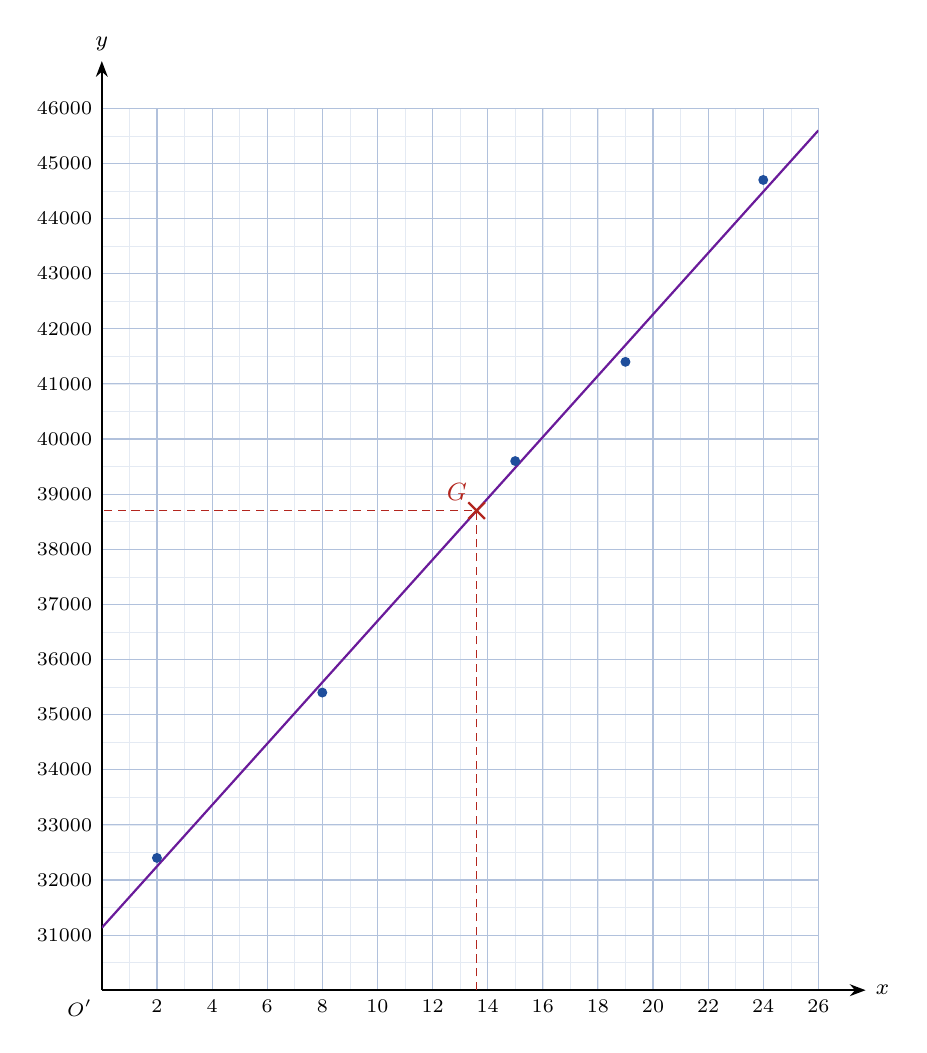
\begin{tikzpicture}[font=\footnotesize]
\draw[cDef!12,very thin](0.000,0)--(0.000,11.200);
\draw[cDef!12,very thin](0.350,0)--(0.350,11.200);
\draw[cDef!12,very thin](0.700,0)--(0.700,11.200);
\draw[cDef!12,very thin](1.050,0)--(1.050,11.200);
\draw[cDef!12,very thin](1.400,0)--(1.400,11.200);
\draw[cDef!12,very thin](1.750,0)--(1.750,11.200);
\draw[cDef!12,very thin](2.100,0)--(2.100,11.200);
\draw[cDef!12,very thin](2.450,0)--(2.450,11.200);
\draw[cDef!12,very thin](2.800,0)--(2.800,11.200);
\draw[cDef!12,very thin](3.150,0)--(3.150,11.200);
\draw[cDef!12,very thin](3.500,0)--(3.500,11.200);
\draw[cDef!12,very thin](3.850,0)--(3.850,11.200);
\draw[cDef!12,very thin](4.200,0)--(4.200,11.200);
\draw[cDef!12,very thin](4.550,0)--(4.550,11.200);
\draw[cDef!12,very thin](4.900,0)--(4.900,11.200);
\draw[cDef!12,very thin](5.250,0)--(5.250,11.200);
\draw[cDef!12,very thin](5.600,0)--(5.600,11.200);
\draw[cDef!12,very thin](5.950,0)--(5.950,11.200);
\draw[cDef!12,very thin](6.300,0)--(6.300,11.200);
\draw[cDef!12,very thin](6.650,0)--(6.650,11.200);
\draw[cDef!12,very thin](7.000,0)--(7.000,11.200);
\draw[cDef!12,very thin](7.350,0)--(7.350,11.200);
\draw[cDef!12,very thin](7.700,0)--(7.700,11.200);
\draw[cDef!12,very thin](8.050,0)--(8.050,11.200);
\draw[cDef!12,very thin](8.400,0)--(8.400,11.200);
\draw[cDef!12,very thin](8.750,0)--(8.750,11.200);
\draw[cDef!12,very thin](9.100,0)--(9.100,11.200);
\draw[cDef!12,very thin](0,0.000)--(9.100,0.000);
\draw[cDef!12,very thin](0,0.350)--(9.100,0.350);
\draw[cDef!12,very thin](0,0.700)--(9.100,0.700);
\draw[cDef!12,very thin](0,1.050)--(9.100,1.050);
\draw[cDef!12,very thin](0,1.400)--(9.100,1.400);
\draw[cDef!12,very thin](0,1.750)--(9.100,1.750);
\draw[cDef!12,very thin](0,2.100)--(9.100,2.100);
\draw[cDef!12,very thin](0,2.450)--(9.100,2.450);
\draw[cDef!12,very thin](0,2.800)--(9.100,2.800);
\draw[cDef!12,very thin](0,3.150)--(9.100,3.150);
\draw[cDef!12,very thin](0,3.500)--(9.100,3.500);
\draw[cDef!12,very thin](0,3.850)--(9.100,3.850);
\draw[cDef!12,very thin](0,4.200)--(9.100,4.200);
\draw[cDef!12,very thin](0,4.550)--(9.100,4.550);
\draw[cDef!12,very thin](0,4.900)--(9.100,4.900);
\draw[cDef!12,very thin](0,5.250)--(9.100,5.250);
\draw[cDef!12,very thin](0,5.600)--(9.100,5.600);
\draw[cDef!12,very thin](0,5.950)--(9.100,5.950);
\draw[cDef!12,very thin](0,6.300)--(9.100,6.300);
\draw[cDef!12,very thin](0,6.650)--(9.100,6.650);
\draw[cDef!12,very thin](0,7.000)--(9.100,7.000);
\draw[cDef!12,very thin](0,7.350)--(9.100,7.350);
\draw[cDef!12,very thin](0,7.700)--(9.100,7.700);
\draw[cDef!12,very thin](0,8.050)--(9.100,8.050);
\draw[cDef!12,very thin](0,8.400)--(9.100,8.400);
\draw[cDef!12,very thin](0,8.750)--(9.100,8.750);
\draw[cDef!12,very thin](0,9.100)--(9.100,9.100);
\draw[cDef!12,very thin](0,9.450)--(9.100,9.450);
\draw[cDef!12,very thin](0,9.800)--(9.100,9.800);
\draw[cDef!12,very thin](0,10.150)--(9.100,10.150);
\draw[cDef!12,very thin](0,10.500)--(9.100,10.500);
\draw[cDef!12,very thin](0,10.850)--(9.100,10.850);
\draw[cDef!12,very thin](0,11.200)--(9.100,11.200);
\draw[cDef!35,thin](0.000,0)--(0.000,11.200);
\draw[cDef!35,thin](0.700,0)--(0.700,11.200);
\draw[cDef!35,thin](1.400,0)--(1.400,11.200);
\draw[cDef!35,thin](2.100,0)--(2.100,11.200);
\draw[cDef!35,thin](2.800,0)--(2.800,11.200);
\draw[cDef!35,thin](3.500,0)--(3.500,11.200);
\draw[cDef!35,thin](4.200,0)--(4.200,11.200);
\draw[cDef!35,thin](4.900,0)--(4.900,11.200);
\draw[cDef!35,thin](5.600,0)--(5.600,11.200);
\draw[cDef!35,thin](6.300,0)--(6.300,11.200);
\draw[cDef!35,thin](7.000,0)--(7.000,11.200);
\draw[cDef!35,thin](7.700,0)--(7.700,11.200);
\draw[cDef!35,thin](8.400,0)--(8.400,11.200);
\draw[cDef!35,thin](9.100,0)--(9.100,11.200);
\draw[cDef!35,thin](0,0.000)--(9.100,0.000);
\draw[cDef!35,thin](0,0.700)--(9.100,0.700);
\draw[cDef!35,thin](0,1.400)--(9.100,1.400);
\draw[cDef!35,thin](0,2.100)--(9.100,2.100);
\draw[cDef!35,thin](0,2.800)--(9.100,2.800);
\draw[cDef!35,thin](0,3.500)--(9.100,3.500);
\draw[cDef!35,thin](0,4.200)--(9.100,4.200);
\draw[cDef!35,thin](0,4.900)--(9.100,4.900);
\draw[cDef!35,thin](0,5.600)--(9.100,5.600);
\draw[cDef!35,thin](0,6.300)--(9.100,6.300);
\draw[cDef!35,thin](0,7.000)--(9.100,7.000);
\draw[cDef!35,thin](0,7.700)--(9.100,7.700);
\draw[cDef!35,thin](0,8.400)--(9.100,8.400);
\draw[cDef!35,thin](0,9.100)--(9.100,9.100);
\draw[cDef!35,thin](0,9.800)--(9.100,9.800);
\draw[cDef!35,thin](0,10.500)--(9.100,10.500);
\draw[cDef!35,thin](0,11.200)--(9.100,11.200);
\draw[-{Stealth[length=2mm]},thick](0,0)--(9.700,0) node[right]{$x$};
\draw[-{Stealth[length=2mm]},thick](0,0)--(0,11.800) node[above]{$y$};
\node[below,font=\scriptsize] at (0.700,0){$2$};
\node[below,font=\scriptsize] at (1.400,0){$4$};
\node[below,font=\scriptsize] at (2.100,0){$6$};
\node[below,font=\scriptsize] at (2.800,0){$8$};
\node[below,font=\scriptsize] at (3.500,0){$10$};
\node[below,font=\scriptsize] at (4.200,0){$12$};
\node[below,font=\scriptsize] at (4.900,0){$14$};
\node[below,font=\scriptsize] at (5.600,0){$16$};
\node[below,font=\scriptsize] at (6.300,0){$18$};
\node[below,font=\scriptsize] at (7.000,0){$20$};
\node[below,font=\scriptsize] at (7.700,0){$22$};
\node[below,font=\scriptsize] at (8.400,0){$24$};
\node[below,font=\scriptsize] at (9.100,0){$26$};
\node[left,font=\scriptsize] at (0,0.700){$31000$};
\node[left,font=\scriptsize] at (0,1.400){$32000$};
\node[left,font=\scriptsize] at (0,2.100){$33000$};
\node[left,font=\scriptsize] at (0,2.800){$34000$};
\node[left,font=\scriptsize] at (0,3.500){$35000$};
\node[left,font=\scriptsize] at (0,4.200){$36000$};
\node[left,font=\scriptsize] at (0,4.900){$37000$};
\node[left,font=\scriptsize] at (0,5.600){$38000$};
\node[left,font=\scriptsize] at (0,6.300){$39000$};
\node[left,font=\scriptsize] at (0,7.000){$40000$};
\node[left,font=\scriptsize] at (0,7.700){$41000$};
\node[left,font=\scriptsize] at (0,8.400){$42000$};
\node[left,font=\scriptsize] at (0,9.100){$43000$};
\node[left,font=\scriptsize] at (0,9.800){$44000$};
\node[left,font=\scriptsize] at (0,10.500){$45000$};
\node[left,font=\scriptsize] at (0,11.200){$46000$};
\node[below left,font=\scriptsize] at (0,0){$O'$};
\begin{scope}\clip(0,0) rectangle (9.100,11.200);
\draw[cMeth,thick](0.000,0.793)--(9.100,10.919);
\end{scope}
\fill[cDef](0.700,1.680) circle (1.8pt);
\fill[cDef](2.800,3.780) circle (1.8pt);
\fill[cDef](5.250,6.720) circle (1.8pt);
\fill[cDef](6.650,7.980) circle (1.8pt);
\fill[cDef](8.400,10.290) circle (1.8pt);
\draw[cThm,densely dashed](4.760,0)--(4.760,6.090)--(0,6.090);
\draw[cThm,thick](4.760,6.090) +(-3pt,-3pt)--+(3pt,3pt) +(-3pt,3pt)--+(3pt,-3pt);
\node[cThm,above left,font=\small\bfseries] at (4.760,6.090){$G$};
\end{tikzpicture}\end{LTR}\end{center}
\pb النقط تكاد تكون على استقامة واحدة (السحابة ممدودة في اتجاه واحد)، لذا يمكن إجراء تعديل خطي. ويؤكد ذلك معامل الارتباط الخطي $r\approx0{,}999$ القريب جدا من $1$.

\QQ{2}
\pa \[\bar x=\frac{2+8+15+19+24}{5}=\frac{68}{5}=13{,}6\qquad \bar y=\frac{193500}{5}=38700\qquad \bx{G(13{,}6\,;\,38700)}\]
\pb جدول الحساب:
\begin{center}\begin{LTR}\renewcommand{\arraystretch}{1.25}
\begin{tabular}{|>{\columncolor{cSec!6}}c|*{5}{c|}>{\columncolor{cEx!10}}c|}\hline
\rowcolor{cSec!12}$x_i$ & 2 & 8 & 15 & 19 & 24 & $68$\\\hline
$y_i$ & 32400 & 35400 & 39600 & 41400 & 44700 & $193500$\\\hline
$x_i^2$ & 4 & 64 & 225 & 361 & 576 & $1230$\\\hline
$x_iy_i$ & 64800 & 283200 & 594000 & 786600 & 1072800 & $2801400$\\\hline
\end{tabular}\end{LTR}\end{center}
\[V(x)=\frac{1230}{5}-13{,}6^{2}=246-184{,}96=61{,}04\]
\[\operatorname{cov}(x,y)=\frac{2801400}{5}-13{,}6\times38700=560280-526320=33960\]
\begin{itemize}
\item $a=\dfrac{33960}{61{,}04}\approx556{,}3565$، إذن \bx{a\approx556{,}356}.
\item $b=\bar y-a\bar x=38700-556{,}356\times13{,}6=38700-7566{,}4416=31133{,}5584$، إذن \bx{b\approx31133{,}558}.
\end{itemize}
\[(D):\ y=556{,}356x+31133{,}558\]

\QQ{3}
\pa من أجل $x=30$: $y=556{,}356\times30+31133{,}558=16690{,}68+31133{,}558=47824{,}238$.

الأجرة المقدّرة: \bxt{حوالي $47824{,}24$ دينارا}.
\pb نحل $556{,}356x+31133{,}558>50000$ أي $x>\dfrac{50000-31133{,}558}{556{,}356}=\dfrac{18866{,}442}{556{,}356}\approx33{,}91$.

إذن تتجاوز الأجرة $50000$ دينار \bxt{بعد 34 سنة من العمل}.
\end{hal}

% ===================== بكالوريا 2011 -- الموضوع الثاني =====================
\begin{tamrin}{بكالوريا 2011 -- الموضوع الثاني -- تسيير واقتصاد}
يمثل الجدول التالي الكميات المنتجة لسلعة شركة من سنة 2006 إلى سنة 2010. (الكميات مقدرة بالطن)
\begin{center}\begin{LTR}\renewcommand{\arraystretch}{1.25}
\begin{tabular}{|>{\columncolor{cSec!6}}c|*{5}{c|}}\hline
\rowcolor{cSec!12}\ar{السنة} & 2006 & 2007 & 2008 & 2009 & 2010\\\hline
\ar{رتبة السنة $x_i$} & 1 & 2 & 3 & 4 & 5\\\hline
\ar{كمية الإنتاج $y_i$} & $2{,}6$ & $2{,}8$ & $3{,}2$ & $4$ & $4{,}4$\\\hline
\end{tabular}\end{LTR}\end{center}
\QQ{1} مثّل سحابة النقط $M_i(x_i;y_i)$ في معلم متعامد. ($2\,cm$ يمثل رتبة واحدة على محور الفواصل، $1\,cm$ يمثل $0{,}4$ طن على محور التراتيب).
\QQ{2} عيّن إحداثيي النقطة المتوسطة $G$ للسحابة ومثّلها في المعلم السابق.
\QQ{3}
\begin{sq}
\qa جد معادلة مستقيم الانحدار بالمربعات الدنيا.
\qb ارسم هذا المستقيم في المعلم السابق.
\end{sq}
\QQ{4} ما هي كمية الإنتاج المتوقعة سنة 2015؟
\end{tamrin}

\Needspace{30\baselineskip}
\begin{hal}
\par\smallskip\textbf{1، 2 و 3(ب).}  السحابة، $G$ والمستقيم $(D)$ (الرسم مصغّر قليلا):
\begin{center}\begin{LTR}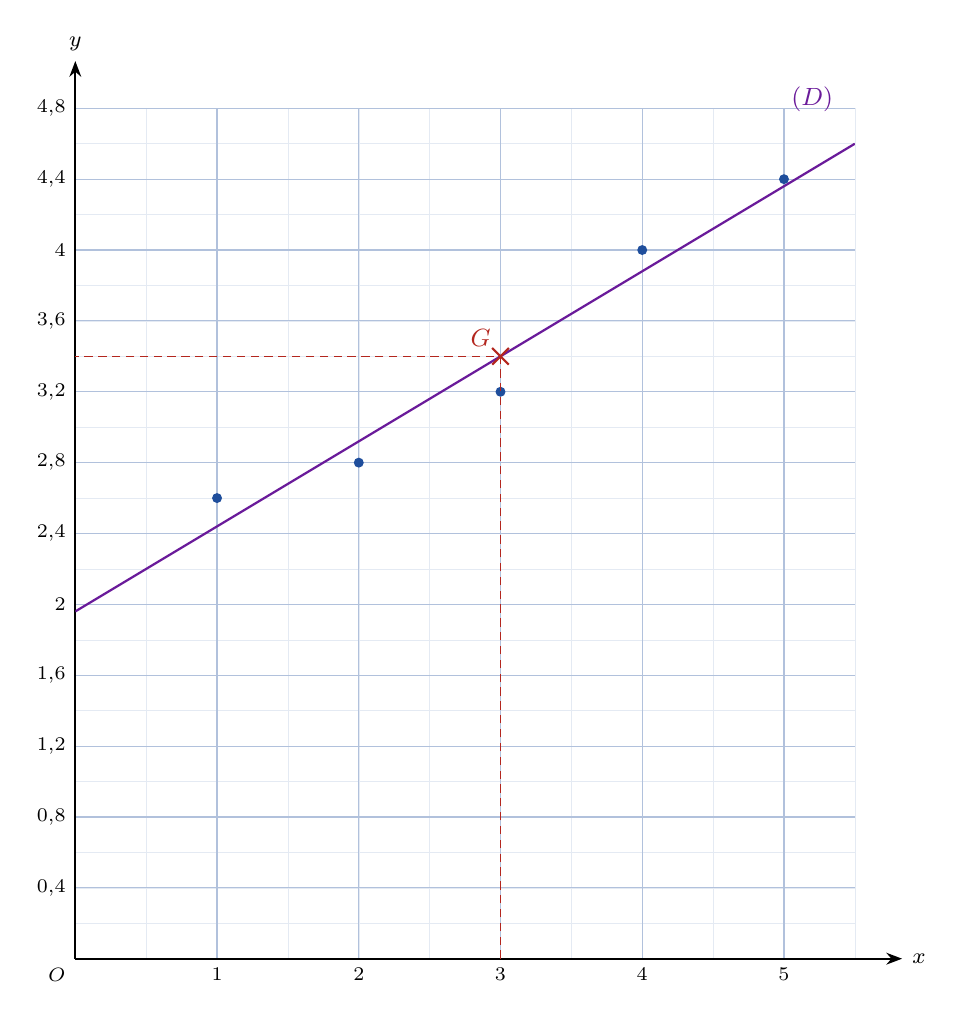
\begin{tikzpicture}[font=\footnotesize]
\draw[cDef!12,very thin](0.000,0)--(0.000,10.800);
\draw[cDef!12,very thin](0.900,0)--(0.900,10.800);
\draw[cDef!12,very thin](1.800,0)--(1.800,10.800);
\draw[cDef!12,very thin](2.700,0)--(2.700,10.800);
\draw[cDef!12,very thin](3.600,0)--(3.600,10.800);
\draw[cDef!12,very thin](4.500,0)--(4.500,10.800);
\draw[cDef!12,very thin](5.400,0)--(5.400,10.800);
\draw[cDef!12,very thin](6.300,0)--(6.300,10.800);
\draw[cDef!12,very thin](7.200,0)--(7.200,10.800);
\draw[cDef!12,very thin](8.100,0)--(8.100,10.800);
\draw[cDef!12,very thin](9.000,0)--(9.000,10.800);
\draw[cDef!12,very thin](9.900,0)--(9.900,10.800);
\draw[cDef!12,very thin](0,0.000)--(9.900,0.000);
\draw[cDef!12,very thin](0,0.450)--(9.900,0.450);
\draw[cDef!12,very thin](0,0.900)--(9.900,0.900);
\draw[cDef!12,very thin](0,1.350)--(9.900,1.350);
\draw[cDef!12,very thin](0,1.800)--(9.900,1.800);
\draw[cDef!12,very thin](0,2.250)--(9.900,2.250);
\draw[cDef!12,very thin](0,2.700)--(9.900,2.700);
\draw[cDef!12,very thin](0,3.150)--(9.900,3.150);
\draw[cDef!12,very thin](0,3.600)--(9.900,3.600);
\draw[cDef!12,very thin](0,4.050)--(9.900,4.050);
\draw[cDef!12,very thin](0,4.500)--(9.900,4.500);
\draw[cDef!12,very thin](0,4.950)--(9.900,4.950);
\draw[cDef!12,very thin](0,5.400)--(9.900,5.400);
\draw[cDef!12,very thin](0,5.850)--(9.900,5.850);
\draw[cDef!12,very thin](0,6.300)--(9.900,6.300);
\draw[cDef!12,very thin](0,6.750)--(9.900,6.750);
\draw[cDef!12,very thin](0,7.200)--(9.900,7.200);
\draw[cDef!12,very thin](0,7.650)--(9.900,7.650);
\draw[cDef!12,very thin](0,8.100)--(9.900,8.100);
\draw[cDef!12,very thin](0,8.550)--(9.900,8.550);
\draw[cDef!12,very thin](0,9.000)--(9.900,9.000);
\draw[cDef!12,very thin](0,9.450)--(9.900,9.450);
\draw[cDef!12,very thin](0,9.900)--(9.900,9.900);
\draw[cDef!12,very thin](0,10.350)--(9.900,10.350);
\draw[cDef!12,very thin](0,10.800)--(9.900,10.800);
\draw[cDef!35,thin](0.000,0)--(0.000,10.800);
\draw[cDef!35,thin](1.800,0)--(1.800,10.800);
\draw[cDef!35,thin](3.600,0)--(3.600,10.800);
\draw[cDef!35,thin](5.400,0)--(5.400,10.800);
\draw[cDef!35,thin](7.200,0)--(7.200,10.800);
\draw[cDef!35,thin](9.000,0)--(9.000,10.800);
\draw[cDef!35,thin](0,0.000)--(9.900,0.000);
\draw[cDef!35,thin](0,0.900)--(9.900,0.900);
\draw[cDef!35,thin](0,1.800)--(9.900,1.800);
\draw[cDef!35,thin](0,2.700)--(9.900,2.700);
\draw[cDef!35,thin](0,3.600)--(9.900,3.600);
\draw[cDef!35,thin](0,4.500)--(9.900,4.500);
\draw[cDef!35,thin](0,5.400)--(9.900,5.400);
\draw[cDef!35,thin](0,6.300)--(9.900,6.300);
\draw[cDef!35,thin](0,7.200)--(9.900,7.200);
\draw[cDef!35,thin](0,8.100)--(9.900,8.100);
\draw[cDef!35,thin](0,9.000)--(9.900,9.000);
\draw[cDef!35,thin](0,9.900)--(9.900,9.900);
\draw[cDef!35,thin](0,10.800)--(9.900,10.800);
\draw[-{Stealth[length=2mm]},thick](0,0)--(10.500,0) node[right]{$x$};
\draw[-{Stealth[length=2mm]},thick](0,0)--(0,11.400) node[above]{$y$};
\node[below,font=\scriptsize] at (1.800,0){$1$};
\node[below,font=\scriptsize] at (3.600,0){$2$};
\node[below,font=\scriptsize] at (5.400,0){$3$};
\node[below,font=\scriptsize] at (7.200,0){$4$};
\node[below,font=\scriptsize] at (9.000,0){$5$};
\node[left,font=\scriptsize] at (0,0.900){$0{,}4$};
\node[left,font=\scriptsize] at (0,1.800){$0{,}8$};
\node[left,font=\scriptsize] at (0,2.700){$1{,}2$};
\node[left,font=\scriptsize] at (0,3.600){$1{,}6$};
\node[left,font=\scriptsize] at (0,4.500){$2$};
\node[left,font=\scriptsize] at (0,5.400){$2{,}4$};
\node[left,font=\scriptsize] at (0,6.300){$2{,}8$};
\node[left,font=\scriptsize] at (0,7.200){$3{,}2$};
\node[left,font=\scriptsize] at (0,8.100){$3{,}6$};
\node[left,font=\scriptsize] at (0,9.000){$4$};
\node[left,font=\scriptsize] at (0,9.900){$4{,}4$};
\node[left,font=\scriptsize] at (0,10.800){$4{,}8$};
\node[below left,font=\scriptsize] at (0,0){$O$};
\begin{scope}\clip(0,0) rectangle (9.900,10.800);
\draw[cMeth,thick](0.000,4.410)--(9.900,10.350);
\end{scope}
\node[cMeth,font=\small] at (9.360,10.912){$(D)$};
\fill[cDef](1.800,5.850) circle (1.8pt);
\fill[cDef](3.600,6.300) circle (1.8pt);
\fill[cDef](5.400,7.200) circle (1.8pt);
\fill[cDef](7.200,9.000) circle (1.8pt);
\fill[cDef](9.000,9.900) circle (1.8pt);
\draw[cThm,densely dashed](5.400,0)--(5.400,7.650)--(0,7.650);
\draw[cThm,thick](5.400,7.650) +(-3pt,-3pt)--+(3pt,3pt) +(-3pt,3pt)--+(3pt,-3pt);
\node[cThm,above left,font=\small\bfseries] at (5.400,7.650){$G$};
\end{tikzpicture}\end{LTR}\end{center}

\QQ{2} \[\bar x=\frac{15}{5}=3\qquad \bar y=\frac{17}{5}=3{,}4\qquad \bx{G(3\,;\,3{,}4)}\]

\QQ{3}
\pa جدول الحساب:
\begin{center}\begin{LTR}\renewcommand{\arraystretch}{1.25}
\begin{tabular}{|>{\columncolor{cSec!6}}c|*{5}{c|}>{\columncolor{cEx!10}}c|}\hline
\rowcolor{cSec!12}$x_i$ & 1 & 2 & 3 & 4 & 5 & $15$\\\hline
$y_i$ & $2{,}6$ & $2{,}8$ & $3{,}2$ & $4$ & $4{,}4$ & $17$\\\hline
$x_i^2$ & 1 & 4 & 9 & 16 & 25 & $55$\\\hline
$x_iy_i$ & $2{,}6$ & $5{,}6$ & $9{,}6$ & $16$ & $22$ & $55{,}8$\\\hline
\end{tabular}\end{LTR}\end{center}
\[V(x)=\frac{55}{5}-3^{2}=11-9=2\]
\[\operatorname{cov}(x,y)=\frac{55{,}8}{5}-3\times3{,}4=11{,}16-10{,}2=0{,}96\]
\[a=\frac{0{,}96}{2}=0{,}48\]
\[b=\bar y-a\bar x=3{,}4-0{,}48\times3=3{,}4-1{,}44=1{,}96\]
\[\bx{(D):\ y=0{,}48x+1{,}96}\]
\pb $(D)$ يشمل $G(3;3{,}4)$ والنقطة $(0;1{,}96)$ (أو $(5;4{,}36)$).

\QQ{4} سنة 2015 توافق الرتبة $x=10$:
\[y=0{,}48\times10+1{,}96=6{,}76\]
الكمية المتوقعة: \bxt{$6{,}76$ طن}.
\end{hal}

% ===================== بكالوريا 2012 -- الموضوع الأول =====================
\begin{tamrin}{بكالوريا 2012 -- الموضوع الأول -- تسيير واقتصاد}
يعطى الجدول أدناه كميات الحليب، مقدرة بالهكتولتر $hL$، التي تم تجميعها في إحدى ولايات الوطن من سنة 2006 إلى 2011:
\begin{center}\begin{LTR}\renewcommand{\arraystretch}{1.25}
\begin{tabular}{|>{\columncolor{cSec!6}}c|*{6}{c|}}\hline
\rowcolor{cSec!12}\ar{السنة} & 2006 & 2007 & 2008 & 2009 & 2010 & 2011\\\hline
\ar{رتبة السنة $x_i$} & 1 & 2 & 3 & 4 & 5 & 6\\\hline
\ar{كمية الحليب المجمعة (بـ $hL$) $y_i$} & 25000 & 26000 & 28500 & 29000 & 31000 & 33498\\\hline
\end{tabular}\end{LTR}\end{center}
\QQ{1} مثّل سحابة النقط $M_i(x_i;y_i)$ في معلم متعامد مبدؤه $O'(0;20000)$ وبوحدة $1\,cm$ لكل سنة على محور الفواصل و $1\,cm$ لكل $2000\,hL$ على محور التراتيب.
\QQ{2}
\begin{sq}
\qa عيّن $G$ النقطة المتوسطة لهذه السحابة.
\qb عيّن معادلة مستقيم الانحدار بالمربعات الدنيا. (تعطى نتائج كل حساب مدوّرة إلى $10^{-2}$)
\end{sq}
\QQ{3} قدّر كمية الحليب التي يمكن تجميعها في سنة 2015 باستعمال التعديل الخطي السابق.
\QQ{4} إذا اعتبرنا أن كمية الحليب المجمعة في السنوات الموالية لسنة 2011 تتم بنفس الوتيرة التي تمت بها من سنة 2006 إلى 2011، فابتداء من أية سنة ستتعدى الكمية المجمعة $50000\,hL$؟
\end{tamrin}

\Needspace{30\baselineskip}
\begin{hal}
\QQ{1} السحابة، $G$ ومستقيم الانحدار $(D)$:
\begin{center}\begin{LTR}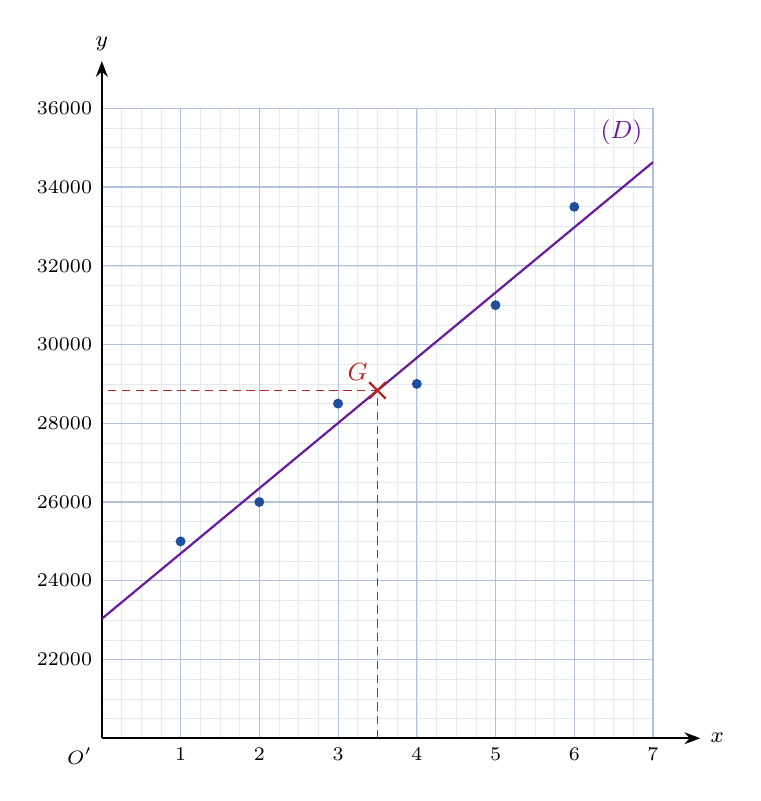
\begin{tikzpicture}[font=\footnotesize]
\draw[cDef!12,very thin](0.000,0)--(0.000,8.000);
\draw[cDef!12,very thin](0.250,0)--(0.250,8.000);
\draw[cDef!12,very thin](0.500,0)--(0.500,8.000);
\draw[cDef!12,very thin](0.750,0)--(0.750,8.000);
\draw[cDef!12,very thin](1.000,0)--(1.000,8.000);
\draw[cDef!12,very thin](1.250,0)--(1.250,8.000);
\draw[cDef!12,very thin](1.500,0)--(1.500,8.000);
\draw[cDef!12,very thin](1.750,0)--(1.750,8.000);
\draw[cDef!12,very thin](2.000,0)--(2.000,8.000);
\draw[cDef!12,very thin](2.250,0)--(2.250,8.000);
\draw[cDef!12,very thin](2.500,0)--(2.500,8.000);
\draw[cDef!12,very thin](2.750,0)--(2.750,8.000);
\draw[cDef!12,very thin](3.000,0)--(3.000,8.000);
\draw[cDef!12,very thin](3.250,0)--(3.250,8.000);
\draw[cDef!12,very thin](3.500,0)--(3.500,8.000);
\draw[cDef!12,very thin](3.750,0)--(3.750,8.000);
\draw[cDef!12,very thin](4.000,0)--(4.000,8.000);
\draw[cDef!12,very thin](4.250,0)--(4.250,8.000);
\draw[cDef!12,very thin](4.500,0)--(4.500,8.000);
\draw[cDef!12,very thin](4.750,0)--(4.750,8.000);
\draw[cDef!12,very thin](5.000,0)--(5.000,8.000);
\draw[cDef!12,very thin](5.250,0)--(5.250,8.000);
\draw[cDef!12,very thin](5.500,0)--(5.500,8.000);
\draw[cDef!12,very thin](5.750,0)--(5.750,8.000);
\draw[cDef!12,very thin](6.000,0)--(6.000,8.000);
\draw[cDef!12,very thin](6.250,0)--(6.250,8.000);
\draw[cDef!12,very thin](6.500,0)--(6.500,8.000);
\draw[cDef!12,very thin](6.750,0)--(6.750,8.000);
\draw[cDef!12,very thin](7.000,0)--(7.000,8.000);
\draw[cDef!12,very thin](0,0.000)--(7.000,0.000);
\draw[cDef!12,very thin](0,0.250)--(7.000,0.250);
\draw[cDef!12,very thin](0,0.500)--(7.000,0.500);
\draw[cDef!12,very thin](0,0.750)--(7.000,0.750);
\draw[cDef!12,very thin](0,1.000)--(7.000,1.000);
\draw[cDef!12,very thin](0,1.250)--(7.000,1.250);
\draw[cDef!12,very thin](0,1.500)--(7.000,1.500);
\draw[cDef!12,very thin](0,1.750)--(7.000,1.750);
\draw[cDef!12,very thin](0,2.000)--(7.000,2.000);
\draw[cDef!12,very thin](0,2.250)--(7.000,2.250);
\draw[cDef!12,very thin](0,2.500)--(7.000,2.500);
\draw[cDef!12,very thin](0,2.750)--(7.000,2.750);
\draw[cDef!12,very thin](0,3.000)--(7.000,3.000);
\draw[cDef!12,very thin](0,3.250)--(7.000,3.250);
\draw[cDef!12,very thin](0,3.500)--(7.000,3.500);
\draw[cDef!12,very thin](0,3.750)--(7.000,3.750);
\draw[cDef!12,very thin](0,4.000)--(7.000,4.000);
\draw[cDef!12,very thin](0,4.250)--(7.000,4.250);
\draw[cDef!12,very thin](0,4.500)--(7.000,4.500);
\draw[cDef!12,very thin](0,4.750)--(7.000,4.750);
\draw[cDef!12,very thin](0,5.000)--(7.000,5.000);
\draw[cDef!12,very thin](0,5.250)--(7.000,5.250);
\draw[cDef!12,very thin](0,5.500)--(7.000,5.500);
\draw[cDef!12,very thin](0,5.750)--(7.000,5.750);
\draw[cDef!12,very thin](0,6.000)--(7.000,6.000);
\draw[cDef!12,very thin](0,6.250)--(7.000,6.250);
\draw[cDef!12,very thin](0,6.500)--(7.000,6.500);
\draw[cDef!12,very thin](0,6.750)--(7.000,6.750);
\draw[cDef!12,very thin](0,7.000)--(7.000,7.000);
\draw[cDef!12,very thin](0,7.250)--(7.000,7.250);
\draw[cDef!12,very thin](0,7.500)--(7.000,7.500);
\draw[cDef!12,very thin](0,7.750)--(7.000,7.750);
\draw[cDef!12,very thin](0,8.000)--(7.000,8.000);
\draw[cDef!35,thin](0.000,0)--(0.000,8.000);
\draw[cDef!35,thin](1.000,0)--(1.000,8.000);
\draw[cDef!35,thin](2.000,0)--(2.000,8.000);
\draw[cDef!35,thin](3.000,0)--(3.000,8.000);
\draw[cDef!35,thin](4.000,0)--(4.000,8.000);
\draw[cDef!35,thin](5.000,0)--(5.000,8.000);
\draw[cDef!35,thin](6.000,0)--(6.000,8.000);
\draw[cDef!35,thin](7.000,0)--(7.000,8.000);
\draw[cDef!35,thin](0,0.000)--(7.000,0.000);
\draw[cDef!35,thin](0,1.000)--(7.000,1.000);
\draw[cDef!35,thin](0,2.000)--(7.000,2.000);
\draw[cDef!35,thin](0,3.000)--(7.000,3.000);
\draw[cDef!35,thin](0,4.000)--(7.000,4.000);
\draw[cDef!35,thin](0,5.000)--(7.000,5.000);
\draw[cDef!35,thin](0,6.000)--(7.000,6.000);
\draw[cDef!35,thin](0,7.000)--(7.000,7.000);
\draw[cDef!35,thin](0,8.000)--(7.000,8.000);
\draw[-{Stealth[length=2mm]},thick](0,0)--(7.600,0) node[right]{$x$};
\draw[-{Stealth[length=2mm]},thick](0,0)--(0,8.600) node[above]{$y$};
\node[below,font=\scriptsize] at (1.000,0){$1$};
\node[below,font=\scriptsize] at (2.000,0){$2$};
\node[below,font=\scriptsize] at (3.000,0){$3$};
\node[below,font=\scriptsize] at (4.000,0){$4$};
\node[below,font=\scriptsize] at (5.000,0){$5$};
\node[below,font=\scriptsize] at (6.000,0){$6$};
\node[below,font=\scriptsize] at (7.000,0){$7$};
\node[left,font=\scriptsize] at (0,1.000){$22000$};
\node[left,font=\scriptsize] at (0,2.000){$24000$};
\node[left,font=\scriptsize] at (0,3.000){$26000$};
\node[left,font=\scriptsize] at (0,4.000){$28000$};
\node[left,font=\scriptsize] at (0,5.000){$30000$};
\node[left,font=\scriptsize] at (0,6.000){$32000$};
\node[left,font=\scriptsize] at (0,7.000){$34000$};
\node[left,font=\scriptsize] at (0,8.000){$36000$};
\node[below left,font=\scriptsize] at (0,0){$O'$};
\begin{scope}\clip(0,0) rectangle (7.000,8.000);
\draw[cMeth,thick](0.000,1.517)--(7.000,7.316);
\end{scope}
\node[cMeth,font=\small] at (6.600,7.700){$(D)$};
\fill[cDef](1.000,2.500) circle (1.8pt);
\fill[cDef](2.000,3.000) circle (1.8pt);
\fill[cDef](3.000,4.250) circle (1.8pt);
\fill[cDef](4.000,4.500) circle (1.8pt);
\fill[cDef](5.000,5.500) circle (1.8pt);
\fill[cDef](6.000,6.749) circle (1.8pt);
\draw[cThm,densely dashed](3.500,0)--(3.500,4.417)--(0,4.417);
\draw[cThm,thick](3.500,4.417) +(-3pt,-3pt)--+(3pt,3pt) +(-3pt,3pt)--+(3pt,-3pt);
\node[cThm,above left,font=\small\bfseries] at (3.500,4.417){$G$};
\end{tikzpicture}\end{LTR}\end{center}

\QQ{2}
\pa \[\bar x=\frac{21}{6}=3{,}5\qquad \bar y=\frac{172998}{6}=28833\qquad \bx{G(3{,}5\,;\,28833)}\]
\pb جدول الحساب:
\begin{center}\begin{LTR}\renewcommand{\arraystretch}{1.25}\small
\begin{tabular}{|>{\columncolor{cSec!6}}c|*{6}{c|}>{\columncolor{cEx!10}}c|}\hline
\rowcolor{cSec!12}$x_i$ & 1 & 2 & 3 & 4 & 5 & 6 & $21$\\\hline
$y_i$ & 25000 & 26000 & 28500 & 29000 & 31000 & 33498 & $172998$\\\hline
$x_i^2$ & 1 & 4 & 9 & 16 & 25 & 36 & $91$\\\hline
$x_iy_i$ & 25000 & 52000 & 85500 & 116000 & 155000 & 200988 & $634488$\\\hline
\end{tabular}\end{LTR}\end{center}
\[V(x)=\frac{91}{6}-3{,}5^{2}=\frac{35}{12}\approx2{,}92\]
\[\operatorname{cov}(x,y)=\frac{634488}{6}-3{,}5\times28833=105748-100915{,}5=4832{,}5\]
\[a=\frac{4832{,}5}{35/12}=\frac{57990}{35}\approx1656{,}86\]
\[b=\bar y-a\bar x=28833-\frac{57990}{35}\times3{,}5=28833-5799=23034\]
\[\bx{(D):\ y=1656{,}86x+23034}\]

\QQ{3} سنة 2015 توافق $x=10$:
\[y=1656{,}86\times10+23034=16568{,}6+23034=39602{,}6\]
الكمية المقدّرة: \bxt{حوالي $39602{,}6\,hL$}.

\QQ{4} «بنفس الوتيرة» تعني بنفس نسبة التطور السنوية المتوسطة. خلال 5 سنوات (من 2006 إلى 2011) ضُربت الكمية في:
\[\frac{33498}{25000}=1{,}33992\]
فإذا كان $q$ المعامل السنوي المتوسط: $q^{5}=1{,}33992$ أي $q=e^{\frac15\ln1{,}33992}\approx e^{0{,}0585}\approx1{,}0603$ (زيادة سنوية حوالي $6\%$).

الكمية بعد $n$ سنة من 2011: $u_n=33498\,q^{n}$. نحل $33498\,q^{n}>50000$:
\[n\ln q>\ln\frac{50000}{33498}\ \Longrightarrow\ n>\frac{\ln1{,}4926}{\ln1{,}0603}\approx\frac{0{,}4005}{0{,}0585}\approx6{,}84\]
إذن $n=7$ (تحقق: $u_6\approx47590<50000$ و $u_7\approx50458>50000$)، أي \bxt{ابتداء من سنة 2018}.
\end{hal}

% ===================== بكالوريا 2013 -- الموضوع الأول =====================
\begin{tamrin}{بكالوريا 2013 -- الموضوع الأول -- تسيير واقتصاد}
الجدول التالي يعطي تطور النسب المئوية من ميزانية إحدى الجامعات، والمخصصة للإنفاق على البحث العلمي بين سنتي 2005 و 2012.
\begin{center}\begin{LTR}\renewcommand{\arraystretch}{1.25}
\begin{tabular}{|>{\columncolor{cSec!6}}c|*{8}{c|}}\hline
\rowcolor{cSec!12}\ar{السنة} & 2005 & 2006 & 2007 & 2008 & 2009 & 2010 & 2011 & 2012\\\hline
\ar{رتبة السنة $x_i$} & 1 & 2 & 3 & 4 & 5 & 6 & 7 & 8\\\hline
\ar{النسبة المئوية $y_i$} & $3{,}3$ & $3{,}8$ & $4{,}5$ & $4{,}7$ & $5$ & $5{,}2$ & $5{,}7$ & $6{,}2$\\\hline
\end{tabular}\end{LTR}\end{center}
\QQ{1} مثّل سحابة النقط $M_i(x_i;y_i)$ في معلم متعامد.
\QQ{2} جد إحداثيي النقطة المتوسطة $G$ لسحابة النقط ثم علّمها.
\QQ{3} بيّن أن المعادلة المختصرة لمستقيم الانحدار بالمربعات الدنيا هي: $y=0{,}38x+3{,}09$، ثم ارسمه.
\QQ{4} بفرض أن تغيّر النسب المئوية يبقى على هذه الوتيرة في السنوات القادمة.
\begin{sq}
\qa قدّر النسبة المئوية لإنفاق هذه الجامعة على البحث العلمي في سنة 2015.
\qb في أية سنة تصبح النسبة المئوية المتوقعة للإنفاق على البحث العلمي لهذه الجامعة هي $9{,}93\%$؟
\end{sq}
\end{tamrin}

\Needspace{30\baselineskip}
\begin{hal}
\QQ{1} النص لم يحدد الوحدات؛ نختار المبدأ $O'(0;3)$، $1{,}5\,cm$ لكل سنة على محور الفواصل و $1\,cm$ لكل $0{,}5\%$ على محور التراتيب:
\begin{center}\begin{LTR}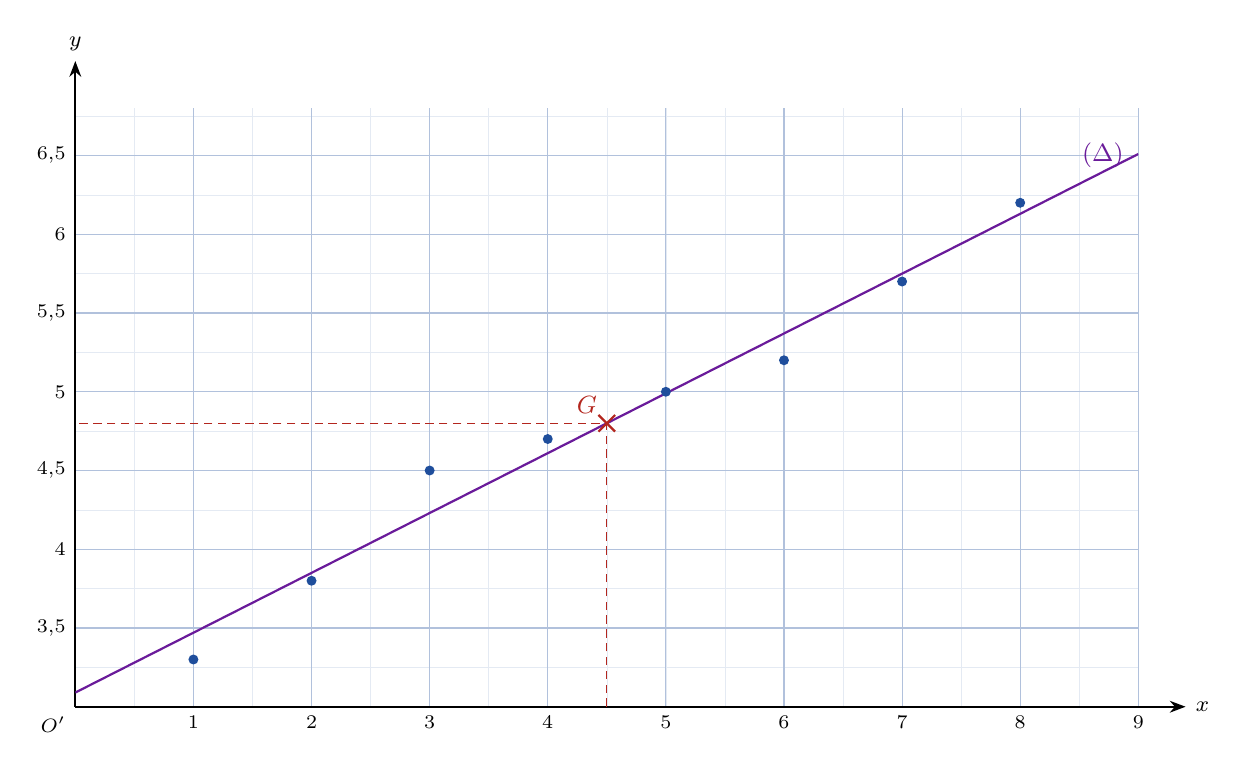
\begin{tikzpicture}[font=\footnotesize]
\draw[cDef!12,very thin](0.000,0)--(0.000,7.600);
\draw[cDef!12,very thin](0.750,0)--(0.750,7.600);
\draw[cDef!12,very thin](1.500,0)--(1.500,7.600);
\draw[cDef!12,very thin](2.250,0)--(2.250,7.600);
\draw[cDef!12,very thin](3.000,0)--(3.000,7.600);
\draw[cDef!12,very thin](3.750,0)--(3.750,7.600);
\draw[cDef!12,very thin](4.500,0)--(4.500,7.600);
\draw[cDef!12,very thin](5.250,0)--(5.250,7.600);
\draw[cDef!12,very thin](6.000,0)--(6.000,7.600);
\draw[cDef!12,very thin](6.750,0)--(6.750,7.600);
\draw[cDef!12,very thin](7.500,0)--(7.500,7.600);
\draw[cDef!12,very thin](8.250,0)--(8.250,7.600);
\draw[cDef!12,very thin](9.000,0)--(9.000,7.600);
\draw[cDef!12,very thin](9.750,0)--(9.750,7.600);
\draw[cDef!12,very thin](10.500,0)--(10.500,7.600);
\draw[cDef!12,very thin](11.250,0)--(11.250,7.600);
\draw[cDef!12,very thin](12.000,0)--(12.000,7.600);
\draw[cDef!12,very thin](12.750,0)--(12.750,7.600);
\draw[cDef!12,very thin](13.500,0)--(13.500,7.600);
\draw[cDef!12,very thin](0,0.000)--(13.500,0.000);
\draw[cDef!12,very thin](0,0.500)--(13.500,0.500);
\draw[cDef!12,very thin](0,1.000)--(13.500,1.000);
\draw[cDef!12,very thin](0,1.500)--(13.500,1.500);
\draw[cDef!12,very thin](0,2.000)--(13.500,2.000);
\draw[cDef!12,very thin](0,2.500)--(13.500,2.500);
\draw[cDef!12,very thin](0,3.000)--(13.500,3.000);
\draw[cDef!12,very thin](0,3.500)--(13.500,3.500);
\draw[cDef!12,very thin](0,4.000)--(13.500,4.000);
\draw[cDef!12,very thin](0,4.500)--(13.500,4.500);
\draw[cDef!12,very thin](0,5.000)--(13.500,5.000);
\draw[cDef!12,very thin](0,5.500)--(13.500,5.500);
\draw[cDef!12,very thin](0,6.000)--(13.500,6.000);
\draw[cDef!12,very thin](0,6.500)--(13.500,6.500);
\draw[cDef!12,very thin](0,7.000)--(13.500,7.000);
\draw[cDef!12,very thin](0,7.500)--(13.500,7.500);
\draw[cDef!35,thin](0.000,0)--(0.000,7.600);
\draw[cDef!35,thin](1.500,0)--(1.500,7.600);
\draw[cDef!35,thin](3.000,0)--(3.000,7.600);
\draw[cDef!35,thin](4.500,0)--(4.500,7.600);
\draw[cDef!35,thin](6.000,0)--(6.000,7.600);
\draw[cDef!35,thin](7.500,0)--(7.500,7.600);
\draw[cDef!35,thin](9.000,0)--(9.000,7.600);
\draw[cDef!35,thin](10.500,0)--(10.500,7.600);
\draw[cDef!35,thin](12.000,0)--(12.000,7.600);
\draw[cDef!35,thin](13.500,0)--(13.500,7.600);
\draw[cDef!35,thin](0,0.000)--(13.500,0.000);
\draw[cDef!35,thin](0,1.000)--(13.500,1.000);
\draw[cDef!35,thin](0,2.000)--(13.500,2.000);
\draw[cDef!35,thin](0,3.000)--(13.500,3.000);
\draw[cDef!35,thin](0,4.000)--(13.500,4.000);
\draw[cDef!35,thin](0,5.000)--(13.500,5.000);
\draw[cDef!35,thin](0,6.000)--(13.500,6.000);
\draw[cDef!35,thin](0,7.000)--(13.500,7.000);
\draw[-{Stealth[length=2mm]},thick](0,0)--(14.100,0) node[right]{$x$};
\draw[-{Stealth[length=2mm]},thick](0,0)--(0,8.200) node[above]{$y$};
\node[below,font=\scriptsize] at (1.500,0){$1$};
\node[below,font=\scriptsize] at (3.000,0){$2$};
\node[below,font=\scriptsize] at (4.500,0){$3$};
\node[below,font=\scriptsize] at (6.000,0){$4$};
\node[below,font=\scriptsize] at (7.500,0){$5$};
\node[below,font=\scriptsize] at (9.000,0){$6$};
\node[below,font=\scriptsize] at (10.500,0){$7$};
\node[below,font=\scriptsize] at (12.000,0){$8$};
\node[below,font=\scriptsize] at (13.500,0){$9$};
\node[left,font=\scriptsize] at (0,1.000){$3{,}5$};
\node[left,font=\scriptsize] at (0,2.000){$4$};
\node[left,font=\scriptsize] at (0,3.000){$4{,}5$};
\node[left,font=\scriptsize] at (0,4.000){$5$};
\node[left,font=\scriptsize] at (0,5.000){$5{,}5$};
\node[left,font=\scriptsize] at (0,6.000){$6$};
\node[left,font=\scriptsize] at (0,7.000){$6{,}5$};
\node[below left,font=\scriptsize] at (0,0){$O'$};
\begin{scope}\clip(0,0) rectangle (13.500,7.600);
\draw[cMeth,thick](0.000,0.180)--(13.500,7.020);
\end{scope}
\node[cMeth,font=\small] at (13.050,7.000){$(\Delta)$};
\fill[cDef](1.500,0.600) circle (1.8pt);
\fill[cDef](3.000,1.600) circle (1.8pt);
\fill[cDef](4.500,3.000) circle (1.8pt);
\fill[cDef](6.000,3.400) circle (1.8pt);
\fill[cDef](7.500,4.000) circle (1.8pt);
\fill[cDef](9.000,4.400) circle (1.8pt);
\fill[cDef](10.500,5.400) circle (1.8pt);
\fill[cDef](12.000,6.400) circle (1.8pt);
\draw[cThm,densely dashed](6.750,0)--(6.750,3.600)--(0,3.600);
\draw[cThm,thick](6.750,3.600) +(-3pt,-3pt)--+(3pt,3pt) +(-3pt,3pt)--+(3pt,-3pt);
\node[cThm,above left,font=\small\bfseries] at (6.750,3.600){$G$};
\end{tikzpicture}\end{LTR}\end{center}

\QQ{2} \[\bar x=\frac{36}{8}=4{,}5\qquad \bar y=\frac{38{,}4}{8}=4{,}8\qquad \bx{G(4{,}5\,;\,4{,}8)}\]

\QQ{3} جدول الحساب:
\begin{center}\begin{LTR}\renewcommand{\arraystretch}{1.25}
\begin{tabular}{|>{\columncolor{cSec!6}}c|*{8}{c|}>{\columncolor{cEx!10}}c|}\hline
\rowcolor{cSec!12}$x_i$ & 1 & 2 & 3 & 4 & 5 & 6 & 7 & 8 & $36$\\\hline
$y_i$ & $3{,}3$ & $3{,}8$ & $4{,}5$ & $4{,}7$ & $5$ & $5{,}2$ & $5{,}7$ & $6{,}2$ & $38{,}4$\\\hline
$x_i^2$ & 1 & 4 & 9 & 16 & 25 & 36 & 49 & 64 & $204$\\\hline
$x_iy_i$ & $3{,}3$ & $7{,}6$ & $13{,}5$ & $18{,}8$ & $25$ & $31{,}2$ & $39{,}9$ & $49{,}6$ & $188{,}9$\\\hline
\end{tabular}\end{LTR}\end{center}
\[V(x)=\frac{204}{8}-4{,}5^{2}=5{,}25\]
\[\operatorname{cov}(x,y)=\frac{188{,}9}{8}-4{,}5\times4{,}8=23{,}6125-21{,}6=2{,}0125\]
\[a=\frac{2{,}0125}{5{,}25}\approx0{,}3833\approx0{,}38\]
\[b=\bar y-a\bar x=4{,}8-0{,}38\times4{,}5=4{,}8-1{,}71=3{,}09\]
\[\bx{(\Delta):\ y=0{,}38x+3{,}09}\]
لرسمه: يشمل $G(4{,}5;4{,}8)$ والنقطة $(0;3{,}09)$ (أو $(8;6{,}13)$).

\QQ{4}
\pa سنة 2015 توافق الرتبة $x=2015-2004=11$:
\[y=0{,}38\times11+3{,}09=4{,}18+3{,}09=7{,}27\]
النسبة المقدّرة: \bx{7{,}27\,\%}.
\pb نحل $0{,}38x+3{,}09=9{,}93$ أي $x=\dfrac{9{,}93-3{,}09}{0{,}38}=\dfrac{6{,}84}{0{,}38}=18$، والرتبة 18 توافق السنة $2004+18=2022$: \bxt{في سنة 2022}.
\end{hal}

% ===================== بكالوريا 2013 -- الموضوع الثاني =====================
\begin{tamrin}{بكالوريا 2013 -- الموضوع الثاني -- تسيير واقتصاد}
الجدول التالي يعطي تطور عدد مستعملي الهاتف النقال في مدينة ما من سنة 2006 إلى سنة 2012:
\begin{center}\begin{LTR}\renewcommand{\arraystretch}{1.25}\small
\begin{tabular}{|>{\columncolor{cSec!6}}c|*{7}{c|}}\hline
\rowcolor{cSec!12}\ar{السنة} & 2006 & 2007 & 2008 & 2009 & 2010 & 2011 & 2012\\\hline
\ar{رتبة السنة $x_i$} & 1 & 2 & 3 & 4 & 5 & 6 & 7\\\hline
\ar{عدد المستعملين $y_i$} & 21400 & 32400 & 48000 & 75600 & 121200 & 207000 & 280000\\\hline
\end{tabular}\end{LTR}\end{center}
\QQ{1}
\begin{sq}
\qa مثّل سحابة النقط $M_i(x_i;y_i)$ في معلم متعامد. (نأخذ على محور الفواصل $1\,cm$ لكل سنة وعلى محور التراتيب $1\,cm$ لكل 20000 مستعمل)
\qb هل يمكن تسوية سحابة النقط السابقة بتعديل خطي؟ برّر إجابتك.
\end{sq}
\QQ{2} بوضع $z_i=\ln y_i$ من أجل $i\in\{1;2;3;4;5;6;7\}$. (تدوّر النتائج إلى $10^{-2}$)
\begin{sq}
\qa انقل الجدول التالي على ورقة الإجابة، ثم أكمله:
\begin{center}\begin{LTR}\renewcommand{\arraystretch}{1.25}
\begin{tabular}{|>{\columncolor{cSec!6}}c|*{7}{p{0.9cm}|}}\hline
\rowcolor{cSec!12}$x_i$ & 1 & 2 & 3 & 4 & 5 & 6 & 7\\\hline
$z_i=\ln y_i$ &&&&&&&\\\hline
\end{tabular}\end{LTR}\end{center}
\qb مثّل سحابة النقط $M'_i(x_i;y_i)$ في معلم متعامد آخر مبدؤه $O'(0;9)$ وبوحدة $1\,cm$ لكل سنة على محور الفواصل و $5\,cm$ لكل وحدة على محور التراتيب.
\qc جد إحداثيي $G$ النقطة المتوسطة لسحابة النقط $M'_i(x_i;y_i)$.
\qd بيّن أن معادلة مستقيم الانحدار بالمربعات الدنيا للسلسلة $(x_i;z_i)$ هي: $z=0{,}44x+9{,}51$.
\end{sq}
\QQ{3}
\begin{sq}
\qa تحقق أن: $y=ke^{0{,}44x}$، حيث $k$ عدد حقيقي يطلب تعيينه. (تدوّر النتيجة إلى الوحدة)
\qb بفرض أن عدد مستعملي الهاتف النقال بهذه المدينة يتزايد بنفس الوتيرة، قدّر عددهم سنة 2014.
\end{sq}
\end{tamrin}

\Needspace{30\baselineskip}
\begin{hal}
\begin{molahada}
في السؤالين 2(ب) و 2(جـ) المقصود السحابة $M'_i(x_i;z_i)$ وليس $M'_i(x_i;y_i)$ (المبدأ $O'(0;9)$ و $5\,cm$ للوحدة يناسبان قيم $z_i$ بين $9{,}97$ و $12{,}54$). نسمّي نقطتها المتوسطة $G'$.
\end{molahada}
\QQ{1}
\pa سحابة النقط (الرسم مصغّر بنسبة $0{,}75$):
\begin{center}\begin{LTR}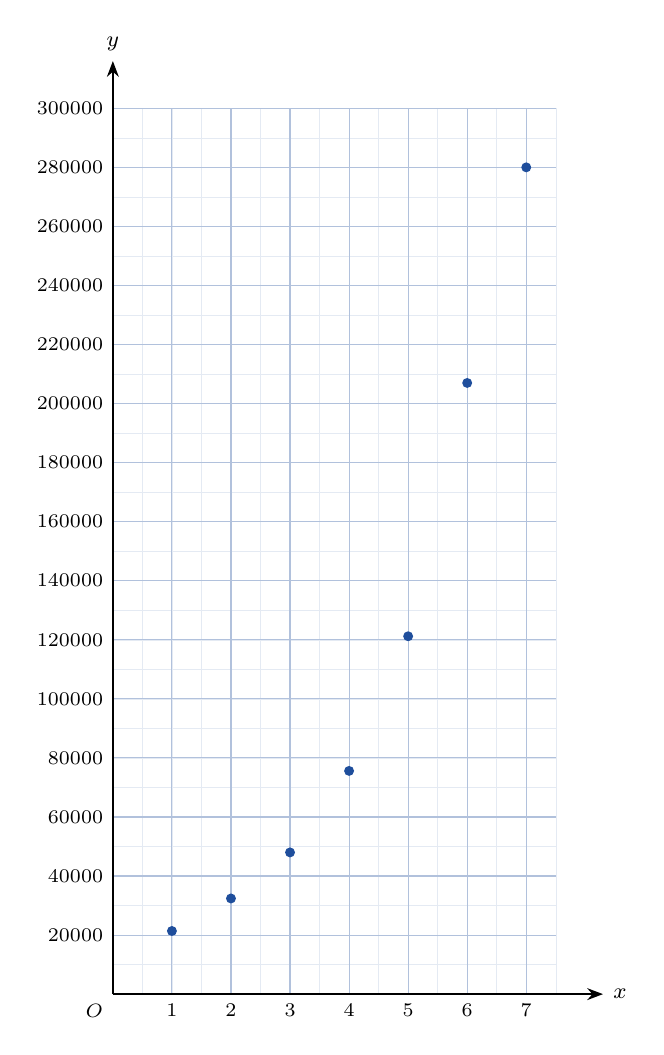
\begin{tikzpicture}[font=\footnotesize]
\draw[cDef!12,very thin](0.000,0)--(0.000,11.250);
\draw[cDef!12,very thin](0.375,0)--(0.375,11.250);
\draw[cDef!12,very thin](0.750,0)--(0.750,11.250);
\draw[cDef!12,very thin](1.125,0)--(1.125,11.250);
\draw[cDef!12,very thin](1.500,0)--(1.500,11.250);
\draw[cDef!12,very thin](1.875,0)--(1.875,11.250);
\draw[cDef!12,very thin](2.250,0)--(2.250,11.250);
\draw[cDef!12,very thin](2.625,0)--(2.625,11.250);
\draw[cDef!12,very thin](3.000,0)--(3.000,11.250);
\draw[cDef!12,very thin](3.375,0)--(3.375,11.250);
\draw[cDef!12,very thin](3.750,0)--(3.750,11.250);
\draw[cDef!12,very thin](4.125,0)--(4.125,11.250);
\draw[cDef!12,very thin](4.500,0)--(4.500,11.250);
\draw[cDef!12,very thin](4.875,0)--(4.875,11.250);
\draw[cDef!12,very thin](5.250,0)--(5.250,11.250);
\draw[cDef!12,very thin](5.625,0)--(5.625,11.250);
\draw[cDef!12,very thin](0,0.000)--(5.625,0.000);
\draw[cDef!12,very thin](0,0.375)--(5.625,0.375);
\draw[cDef!12,very thin](0,0.750)--(5.625,0.750);
\draw[cDef!12,very thin](0,1.125)--(5.625,1.125);
\draw[cDef!12,very thin](0,1.500)--(5.625,1.500);
\draw[cDef!12,very thin](0,1.875)--(5.625,1.875);
\draw[cDef!12,very thin](0,2.250)--(5.625,2.250);
\draw[cDef!12,very thin](0,2.625)--(5.625,2.625);
\draw[cDef!12,very thin](0,3.000)--(5.625,3.000);
\draw[cDef!12,very thin](0,3.375)--(5.625,3.375);
\draw[cDef!12,very thin](0,3.750)--(5.625,3.750);
\draw[cDef!12,very thin](0,4.125)--(5.625,4.125);
\draw[cDef!12,very thin](0,4.500)--(5.625,4.500);
\draw[cDef!12,very thin](0,4.875)--(5.625,4.875);
\draw[cDef!12,very thin](0,5.250)--(5.625,5.250);
\draw[cDef!12,very thin](0,5.625)--(5.625,5.625);
\draw[cDef!12,very thin](0,6.000)--(5.625,6.000);
\draw[cDef!12,very thin](0,6.375)--(5.625,6.375);
\draw[cDef!12,very thin](0,6.750)--(5.625,6.750);
\draw[cDef!12,very thin](0,7.125)--(5.625,7.125);
\draw[cDef!12,very thin](0,7.500)--(5.625,7.500);
\draw[cDef!12,very thin](0,7.875)--(5.625,7.875);
\draw[cDef!12,very thin](0,8.250)--(5.625,8.250);
\draw[cDef!12,very thin](0,8.625)--(5.625,8.625);
\draw[cDef!12,very thin](0,9.000)--(5.625,9.000);
\draw[cDef!12,very thin](0,9.375)--(5.625,9.375);
\draw[cDef!12,very thin](0,9.750)--(5.625,9.750);
\draw[cDef!12,very thin](0,10.125)--(5.625,10.125);
\draw[cDef!12,very thin](0,10.500)--(5.625,10.500);
\draw[cDef!12,very thin](0,10.875)--(5.625,10.875);
\draw[cDef!12,very thin](0,11.250)--(5.625,11.250);
\draw[cDef!35,thin](0.000,0)--(0.000,11.250);
\draw[cDef!35,thin](0.750,0)--(0.750,11.250);
\draw[cDef!35,thin](1.500,0)--(1.500,11.250);
\draw[cDef!35,thin](2.250,0)--(2.250,11.250);
\draw[cDef!35,thin](3.000,0)--(3.000,11.250);
\draw[cDef!35,thin](3.750,0)--(3.750,11.250);
\draw[cDef!35,thin](4.500,0)--(4.500,11.250);
\draw[cDef!35,thin](5.250,0)--(5.250,11.250);
\draw[cDef!35,thin](0,0.000)--(5.625,0.000);
\draw[cDef!35,thin](0,0.750)--(5.625,0.750);
\draw[cDef!35,thin](0,1.500)--(5.625,1.500);
\draw[cDef!35,thin](0,2.250)--(5.625,2.250);
\draw[cDef!35,thin](0,3.000)--(5.625,3.000);
\draw[cDef!35,thin](0,3.750)--(5.625,3.750);
\draw[cDef!35,thin](0,4.500)--(5.625,4.500);
\draw[cDef!35,thin](0,5.250)--(5.625,5.250);
\draw[cDef!35,thin](0,6.000)--(5.625,6.000);
\draw[cDef!35,thin](0,6.750)--(5.625,6.750);
\draw[cDef!35,thin](0,7.500)--(5.625,7.500);
\draw[cDef!35,thin](0,8.250)--(5.625,8.250);
\draw[cDef!35,thin](0,9.000)--(5.625,9.000);
\draw[cDef!35,thin](0,9.750)--(5.625,9.750);
\draw[cDef!35,thin](0,10.500)--(5.625,10.500);
\draw[cDef!35,thin](0,11.250)--(5.625,11.250);
\draw[-{Stealth[length=2mm]},thick](0,0)--(6.225,0) node[right]{$x$};
\draw[-{Stealth[length=2mm]},thick](0,0)--(0,11.850) node[above]{$y$};
\node[below,font=\scriptsize] at (0.750,0){$1$};
\node[below,font=\scriptsize] at (1.500,0){$2$};
\node[below,font=\scriptsize] at (2.250,0){$3$};
\node[below,font=\scriptsize] at (3.000,0){$4$};
\node[below,font=\scriptsize] at (3.750,0){$5$};
\node[below,font=\scriptsize] at (4.500,0){$6$};
\node[below,font=\scriptsize] at (5.250,0){$7$};
\node[left,font=\scriptsize] at (0,0.750){$20000$};
\node[left,font=\scriptsize] at (0,1.500){$40000$};
\node[left,font=\scriptsize] at (0,2.250){$60000$};
\node[left,font=\scriptsize] at (0,3.000){$80000$};
\node[left,font=\scriptsize] at (0,3.750){$100000$};
\node[left,font=\scriptsize] at (0,4.500){$120000$};
\node[left,font=\scriptsize] at (0,5.250){$140000$};
\node[left,font=\scriptsize] at (0,6.000){$160000$};
\node[left,font=\scriptsize] at (0,6.750){$180000$};
\node[left,font=\scriptsize] at (0,7.500){$200000$};
\node[left,font=\scriptsize] at (0,8.250){$220000$};
\node[left,font=\scriptsize] at (0,9.000){$240000$};
\node[left,font=\scriptsize] at (0,9.750){$260000$};
\node[left,font=\scriptsize] at (0,10.500){$280000$};
\node[left,font=\scriptsize] at (0,11.250){$300000$};
\node[below left,font=\scriptsize] at (0,0){$O$};
\begin{scope}\clip(0,0) rectangle (5.625,11.250);
\end{scope}
\fill[cDef](0.750,0.802) circle (1.8pt);
\fill[cDef](1.500,1.215) circle (1.8pt);
\fill[cDef](2.250,1.800) circle (1.8pt);
\fill[cDef](3.000,2.835) circle (1.8pt);
\fill[cDef](3.750,4.545) circle (1.8pt);
\fill[cDef](4.500,7.762) circle (1.8pt);
\fill[cDef](5.250,10.500) circle (1.8pt);
\end{tikzpicture}\end{LTR}\end{center}
\pb \textbf{لا}: النقط لا تتوزع حول مستقيم، بل تشكّل منحنى يتزايد بسرعة متسارعة (الزيادات السنوية تكبر عموما: من $11000$ إلى $85800$)، بينما النسبة $\dfrac{y_{i+1}}{y_i}$ متقاربة (بين $1{,}35$ و $1{,}71$): التطور أسّي، فالتعديل الخطي غير ملائم.

\QQ{2}
\pa $z_i=\ln y_i$ مدوّرة إلى $10^{-2}$:
\begin{center}\begin{LTR}\renewcommand{\arraystretch}{1.25}
\begin{tabular}{|>{\columncolor{cSec!6}}c|*{7}{c|}}\hline
\rowcolor{cSec!12}$x_i$ & 1 & 2 & 3 & 4 & 5 & 6 & 7\\\hline
$z_i=\ln y_i$ & $9{,}97$ & $10{,}39$ & $10{,}78$ & $11{,}23$ & $11{,}71$ & $12{,}24$ & $12{,}54$\\\hline
\end{tabular}\end{LTR}\end{center}
\pb سحابة النقط $M'_i(x_i;z_i)$، النقطة $G'$ والمستقيم $z=0{,}44x+9{,}51$ (المبدأ $O'(0;9)$، الرسم مصغّر بنسبة $0{,}55$):
\begin{center}\begin{LTR}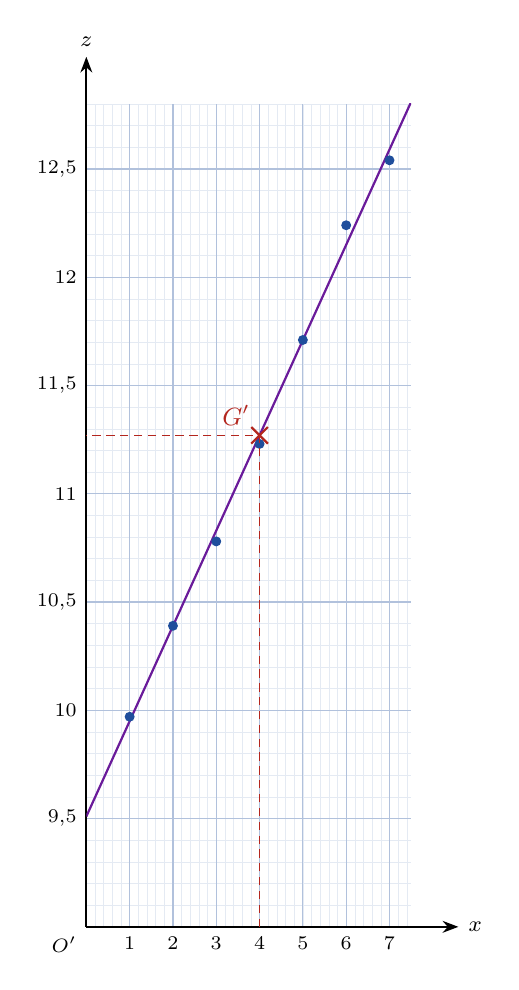
\begin{tikzpicture}[font=\footnotesize]
\draw[cDef!12,very thin](0.000,0)--(0.000,10.450);
\draw[cDef!12,very thin](0.110,0)--(0.110,10.450);
\draw[cDef!12,very thin](0.220,0)--(0.220,10.450);
\draw[cDef!12,very thin](0.330,0)--(0.330,10.450);
\draw[cDef!12,very thin](0.440,0)--(0.440,10.450);
\draw[cDef!12,very thin](0.550,0)--(0.550,10.450);
\draw[cDef!12,very thin](0.660,0)--(0.660,10.450);
\draw[cDef!12,very thin](0.770,0)--(0.770,10.450);
\draw[cDef!12,very thin](0.880,0)--(0.880,10.450);
\draw[cDef!12,very thin](0.990,0)--(0.990,10.450);
\draw[cDef!12,very thin](1.100,0)--(1.100,10.450);
\draw[cDef!12,very thin](1.210,0)--(1.210,10.450);
\draw[cDef!12,very thin](1.320,0)--(1.320,10.450);
\draw[cDef!12,very thin](1.430,0)--(1.430,10.450);
\draw[cDef!12,very thin](1.540,0)--(1.540,10.450);
\draw[cDef!12,very thin](1.650,0)--(1.650,10.450);
\draw[cDef!12,very thin](1.760,0)--(1.760,10.450);
\draw[cDef!12,very thin](1.870,0)--(1.870,10.450);
\draw[cDef!12,very thin](1.980,0)--(1.980,10.450);
\draw[cDef!12,very thin](2.090,0)--(2.090,10.450);
\draw[cDef!12,very thin](2.200,0)--(2.200,10.450);
\draw[cDef!12,very thin](2.310,0)--(2.310,10.450);
\draw[cDef!12,very thin](2.420,0)--(2.420,10.450);
\draw[cDef!12,very thin](2.530,0)--(2.530,10.450);
\draw[cDef!12,very thin](2.640,0)--(2.640,10.450);
\draw[cDef!12,very thin](2.750,0)--(2.750,10.450);
\draw[cDef!12,very thin](2.860,0)--(2.860,10.450);
\draw[cDef!12,very thin](2.970,0)--(2.970,10.450);
\draw[cDef!12,very thin](3.080,0)--(3.080,10.450);
\draw[cDef!12,very thin](3.190,0)--(3.190,10.450);
\draw[cDef!12,very thin](3.300,0)--(3.300,10.450);
\draw[cDef!12,very thin](3.410,0)--(3.410,10.450);
\draw[cDef!12,very thin](3.520,0)--(3.520,10.450);
\draw[cDef!12,very thin](3.630,0)--(3.630,10.450);
\draw[cDef!12,very thin](3.740,0)--(3.740,10.450);
\draw[cDef!12,very thin](3.850,0)--(3.850,10.450);
\draw[cDef!12,very thin](3.960,0)--(3.960,10.450);
\draw[cDef!12,very thin](4.070,0)--(4.070,10.450);
\draw[cDef!12,very thin](0,0.000)--(4.125,0.000);
\draw[cDef!12,very thin](0,0.275)--(4.125,0.275);
\draw[cDef!12,very thin](0,0.550)--(4.125,0.550);
\draw[cDef!12,very thin](0,0.825)--(4.125,0.825);
\draw[cDef!12,very thin](0,1.100)--(4.125,1.100);
\draw[cDef!12,very thin](0,1.375)--(4.125,1.375);
\draw[cDef!12,very thin](0,1.650)--(4.125,1.650);
\draw[cDef!12,very thin](0,1.925)--(4.125,1.925);
\draw[cDef!12,very thin](0,2.200)--(4.125,2.200);
\draw[cDef!12,very thin](0,2.475)--(4.125,2.475);
\draw[cDef!12,very thin](0,2.750)--(4.125,2.750);
\draw[cDef!12,very thin](0,3.025)--(4.125,3.025);
\draw[cDef!12,very thin](0,3.300)--(4.125,3.300);
\draw[cDef!12,very thin](0,3.575)--(4.125,3.575);
\draw[cDef!12,very thin](0,3.850)--(4.125,3.850);
\draw[cDef!12,very thin](0,4.125)--(4.125,4.125);
\draw[cDef!12,very thin](0,4.400)--(4.125,4.400);
\draw[cDef!12,very thin](0,4.675)--(4.125,4.675);
\draw[cDef!12,very thin](0,4.950)--(4.125,4.950);
\draw[cDef!12,very thin](0,5.225)--(4.125,5.225);
\draw[cDef!12,very thin](0,5.500)--(4.125,5.500);
\draw[cDef!12,very thin](0,5.775)--(4.125,5.775);
\draw[cDef!12,very thin](0,6.050)--(4.125,6.050);
\draw[cDef!12,very thin](0,6.325)--(4.125,6.325);
\draw[cDef!12,very thin](0,6.600)--(4.125,6.600);
\draw[cDef!12,very thin](0,6.875)--(4.125,6.875);
\draw[cDef!12,very thin](0,7.150)--(4.125,7.150);
\draw[cDef!12,very thin](0,7.425)--(4.125,7.425);
\draw[cDef!12,very thin](0,7.700)--(4.125,7.700);
\draw[cDef!12,very thin](0,7.975)--(4.125,7.975);
\draw[cDef!12,very thin](0,8.250)--(4.125,8.250);
\draw[cDef!12,very thin](0,8.525)--(4.125,8.525);
\draw[cDef!12,very thin](0,8.800)--(4.125,8.800);
\draw[cDef!12,very thin](0,9.075)--(4.125,9.075);
\draw[cDef!12,very thin](0,9.350)--(4.125,9.350);
\draw[cDef!12,very thin](0,9.625)--(4.125,9.625);
\draw[cDef!12,very thin](0,9.900)--(4.125,9.900);
\draw[cDef!12,very thin](0,10.175)--(4.125,10.175);
\draw[cDef!12,very thin](0,10.450)--(4.125,10.450);
\draw[cDef!35,thin](0.000,0)--(0.000,10.450);
\draw[cDef!35,thin](0.550,0)--(0.550,10.450);
\draw[cDef!35,thin](1.100,0)--(1.100,10.450);
\draw[cDef!35,thin](1.650,0)--(1.650,10.450);
\draw[cDef!35,thin](2.200,0)--(2.200,10.450);
\draw[cDef!35,thin](2.750,0)--(2.750,10.450);
\draw[cDef!35,thin](3.300,0)--(3.300,10.450);
\draw[cDef!35,thin](3.850,0)--(3.850,10.450);
\draw[cDef!35,thin](0,0.000)--(4.125,0.000);
\draw[cDef!35,thin](0,1.375)--(4.125,1.375);
\draw[cDef!35,thin](0,2.750)--(4.125,2.750);
\draw[cDef!35,thin](0,4.125)--(4.125,4.125);
\draw[cDef!35,thin](0,5.500)--(4.125,5.500);
\draw[cDef!35,thin](0,6.875)--(4.125,6.875);
\draw[cDef!35,thin](0,8.250)--(4.125,8.250);
\draw[cDef!35,thin](0,9.625)--(4.125,9.625);
\draw[-{Stealth[length=2mm]},thick](0,0)--(4.725,0) node[right]{$x$};
\draw[-{Stealth[length=2mm]},thick](0,0)--(0,11.050) node[above]{$z$};
\node[below,font=\scriptsize] at (0.550,0){$1$};
\node[below,font=\scriptsize] at (1.100,0){$2$};
\node[below,font=\scriptsize] at (1.650,0){$3$};
\node[below,font=\scriptsize] at (2.200,0){$4$};
\node[below,font=\scriptsize] at (2.750,0){$5$};
\node[below,font=\scriptsize] at (3.300,0){$6$};
\node[below,font=\scriptsize] at (3.850,0){$7$};
\node[left,font=\scriptsize] at (0,1.375){$9{,}5$};
\node[left,font=\scriptsize] at (0,2.750){$10$};
\node[left,font=\scriptsize] at (0,4.125){$10{,}5$};
\node[left,font=\scriptsize] at (0,5.500){$11$};
\node[left,font=\scriptsize] at (0,6.875){$11{,}5$};
\node[left,font=\scriptsize] at (0,8.250){$12$};
\node[left,font=\scriptsize] at (0,9.625){$12{,}5$};
\node[below left,font=\scriptsize] at (0,0){$O'$};
\begin{scope}\clip(0,0) rectangle (4.125,10.450);
\draw[cMeth,thick](0.000,1.402)--(4.125,10.477);
\end{scope}
\fill[cDef](0.550,2.668) circle (1.8pt);
\fill[cDef](1.100,3.823) circle (1.8pt);
\fill[cDef](1.650,4.895) circle (1.8pt);
\fill[cDef](2.200,6.133) circle (1.8pt);
\fill[cDef](2.750,7.453) circle (1.8pt);
\fill[cDef](3.300,8.910) circle (1.8pt);
\fill[cDef](3.850,9.735) circle (1.8pt);
\draw[cThm,densely dashed](2.200,0)--(2.200,6.242)--(0,6.242);
\draw[cThm,thick](2.200,6.242) +(-3pt,-3pt)--+(3pt,3pt) +(-3pt,3pt)--+(3pt,-3pt);
\node[cThm,above left,font=\small\bfseries] at (2.200,6.242){$G'$};
\end{tikzpicture}\end{LTR}\end{center}
\pc \[\bar x=\frac{28}{7}=4\qquad \bar z=\frac{78{,}86}{7}\approx11{,}27\qquad \bx{G'(4\,;\,11{,}27)}\]
\pd جدول الحساب:
\begin{center}\begin{LTR}\renewcommand{\arraystretch}{1.25}
\begin{tabular}{|>{\columncolor{cSec!6}}c|*{7}{c|}>{\columncolor{cEx!10}}c|}\hline
\rowcolor{cSec!12}$x_i$ & 1 & 2 & 3 & 4 & 5 & 6 & 7 & $28$\\\hline
$z_i$ & $9{,}97$ & $10{,}39$ & $10{,}78$ & $11{,}23$ & $11{,}71$ & $12{,}24$ & $12{,}54$ & $78{,}86$\\\hline
$x_i^2$ & 1 & 4 & 9 & 16 & 25 & 36 & 49 & $140$\\\hline
$x_iz_i$ & $9{,}97$ & $20{,}78$ & $32{,}34$ & $44{,}92$ & $58{,}55$ & $73{,}44$ & $87{,}78$ & $327{,}78$\\\hline
\end{tabular}\end{LTR}\end{center}
\[V(x)=\frac{140}{7}-4^{2}=20-16=4\]
\[\operatorname{cov}(x,z)=\frac{327{,}78}{7}-4\times\frac{78{,}86}{7}\approx46{,}8257-45{,}0629=1{,}7629\]
\[a=\frac{1{,}7629}{4}\approx0{,}4407\approx0{,}44\]
\[b=\bar z-a\bar x=11{,}27-0{,}44\times4=11{,}27-1{,}76=9{,}51\]
\[\bx{z=0{,}44x+9{,}51}\]

\QQ{3}
\pa $z=\ln y$ يعني $y=e^{z}=e^{0{,}44x+9{,}51}=e^{9{,}51}\times e^{0{,}44x}$.

إذن $y=ke^{0{,}44x}$ مع $k=e^{9{,}51}\approx13493{,}99$، أي \bx{k\approx13494} و \bx{y=13494\,e^{0{,}44x}}.
\pb سنة 2014 توافق الرتبة $x=2014-2005=9$:
\[y=13494\,e^{0{,}44\times9}=13494\,e^{3{,}96}\approx13494\times52{,}457\approx707859\]
العدد المقدّر سنة 2014: \bxt{حوالي $707859$ مستعملا}.
\end{hal}

% ===================== بكالوريا 2014 -- الموضوع الثاني =====================
\begin{tamrin}{بكالوريا 2014 -- الموضوع الثاني -- تسيير واقتصاد}
الجدول الآتي يمثل تغيّر سعر الكيلوغرام الواحد من مادة استهلاكية بين السنوات 2008 و 2012.
\begin{center}\begin{LTR}\renewcommand{\arraystretch}{1.25}
\begin{tabular}{|>{\columncolor{cSec!6}}c|*{5}{c|}}\hline
\rowcolor{cSec!12}\ar{السنة} & 2008 & 2009 & 2010 & 2011 & 2012\\\hline
\ar{رتبة السنة $x_i$} & 1 & 2 & 3 & 4 & 5\\\hline
\ar{سعر $1\,kg$ بالدولار $y_i$} & $3{,}64$ & $3{,}76$ & $3{,}81$ & $3{,}95$ & $4{,}39$\\\hline
\end{tabular}\end{LTR}\end{center}
\QQ{1} احسب النسبة المئوية لتغيّر سعر الكيلوغرام الواحد من هذه المادة بين سنتي 2008 و 2012.
\QQ{2} مثّل سحابة النقط $M_i(x_i;y_i)$ في معلم متعامد.
\QQ{3} جد إحداثيي $G$ النقطة المتوسطة لسحابة النقط السابقة.
\QQ{4} بيّن أن المعادلة المختصرة لمستقيم الانحدار بالمربعات الدنيا هي: $y=0{,}17x+3{,}40$. (النتائج مدوّرة إلى $10^{-2}$)
\QQ{5} بفرض أن تغيّر سعر الكيلوغرام الواحد من هذه المادة يبقى على نفس الوتيرة في السنوات القادمة.
\begin{sq}
\qa قدّر سعر الكيلوغرام الواحد من هذه المادة في سنة 2016.
\qb في أية سنة سيصبح سعر الكيلوغرام الواحد من هذه المادة الاستهلاكية $5{,}61$ دولارا؟
\end{sq}
\end{tamrin}

\Needspace{30\baselineskip}
\begin{hal}
\QQ{1} \[t=\frac{y_{2012}-y_{2008}}{y_{2008}}\times100=\frac{4{,}39-3{,}64}{3{,}64}\times100=\frac{0{,}75}{3{,}64}\times100\approx20{,}60\]
ارتفع السعر بنسبة \bx{20{,}60\,\%} تقريبا.

\par\smallskip\textbf{2 و 3.}  النص لم يحدد الوحدات؛ نختار المبدأ $O'(0;3{,}5)$، $2\,cm$ لكل سنة و $1\,cm$ لكل $0{,}1$ دولار:
\begin{center}\begin{LTR}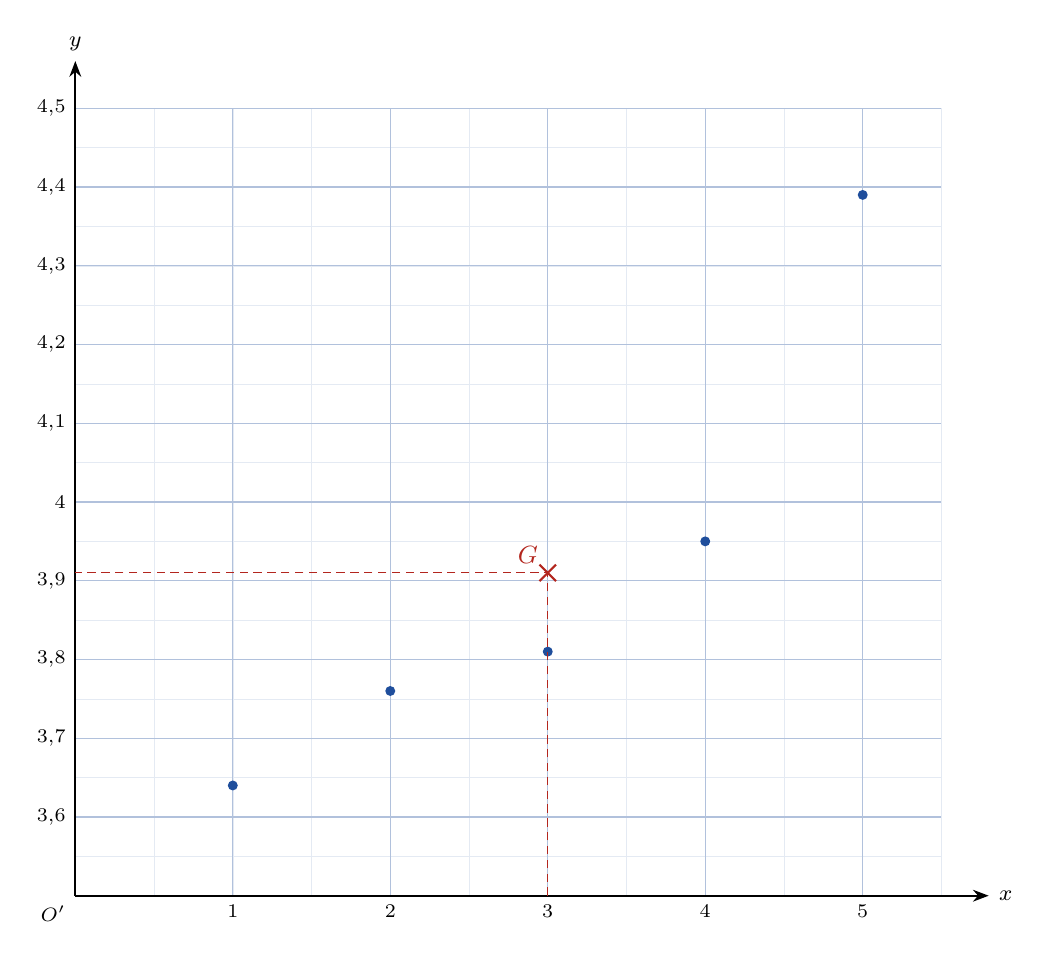
\begin{tikzpicture}[font=\footnotesize]
\draw[cDef!12,very thin](0.000,0)--(0.000,10.000);
\draw[cDef!12,very thin](1.000,0)--(1.000,10.000);
\draw[cDef!12,very thin](2.000,0)--(2.000,10.000);
\draw[cDef!12,very thin](3.000,0)--(3.000,10.000);
\draw[cDef!12,very thin](4.000,0)--(4.000,10.000);
\draw[cDef!12,very thin](5.000,0)--(5.000,10.000);
\draw[cDef!12,very thin](6.000,0)--(6.000,10.000);
\draw[cDef!12,very thin](7.000,0)--(7.000,10.000);
\draw[cDef!12,very thin](8.000,0)--(8.000,10.000);
\draw[cDef!12,very thin](9.000,0)--(9.000,10.000);
\draw[cDef!12,very thin](10.000,0)--(10.000,10.000);
\draw[cDef!12,very thin](11.000,0)--(11.000,10.000);
\draw[cDef!12,very thin](0,0.000)--(11.000,0.000);
\draw[cDef!12,very thin](0,0.500)--(11.000,0.500);
\draw[cDef!12,very thin](0,1.000)--(11.000,1.000);
\draw[cDef!12,very thin](0,1.500)--(11.000,1.500);
\draw[cDef!12,very thin](0,2.000)--(11.000,2.000);
\draw[cDef!12,very thin](0,2.500)--(11.000,2.500);
\draw[cDef!12,very thin](0,3.000)--(11.000,3.000);
\draw[cDef!12,very thin](0,3.500)--(11.000,3.500);
\draw[cDef!12,very thin](0,4.000)--(11.000,4.000);
\draw[cDef!12,very thin](0,4.500)--(11.000,4.500);
\draw[cDef!12,very thin](0,5.000)--(11.000,5.000);
\draw[cDef!12,very thin](0,5.500)--(11.000,5.500);
\draw[cDef!12,very thin](0,6.000)--(11.000,6.000);
\draw[cDef!12,very thin](0,6.500)--(11.000,6.500);
\draw[cDef!12,very thin](0,7.000)--(11.000,7.000);
\draw[cDef!12,very thin](0,7.500)--(11.000,7.500);
\draw[cDef!12,very thin](0,8.000)--(11.000,8.000);
\draw[cDef!12,very thin](0,8.500)--(11.000,8.500);
\draw[cDef!12,very thin](0,9.000)--(11.000,9.000);
\draw[cDef!12,very thin](0,9.500)--(11.000,9.500);
\draw[cDef!12,very thin](0,10.000)--(11.000,10.000);
\draw[cDef!35,thin](0.000,0)--(0.000,10.000);
\draw[cDef!35,thin](2.000,0)--(2.000,10.000);
\draw[cDef!35,thin](4.000,0)--(4.000,10.000);
\draw[cDef!35,thin](6.000,0)--(6.000,10.000);
\draw[cDef!35,thin](8.000,0)--(8.000,10.000);
\draw[cDef!35,thin](10.000,0)--(10.000,10.000);
\draw[cDef!35,thin](0,0.000)--(11.000,0.000);
\draw[cDef!35,thin](0,1.000)--(11.000,1.000);
\draw[cDef!35,thin](0,2.000)--(11.000,2.000);
\draw[cDef!35,thin](0,3.000)--(11.000,3.000);
\draw[cDef!35,thin](0,4.000)--(11.000,4.000);
\draw[cDef!35,thin](0,5.000)--(11.000,5.000);
\draw[cDef!35,thin](0,6.000)--(11.000,6.000);
\draw[cDef!35,thin](0,7.000)--(11.000,7.000);
\draw[cDef!35,thin](0,8.000)--(11.000,8.000);
\draw[cDef!35,thin](0,9.000)--(11.000,9.000);
\draw[cDef!35,thin](0,10.000)--(11.000,10.000);
\draw[-{Stealth[length=2mm]},thick](0,0)--(11.600,0) node[right]{$x$};
\draw[-{Stealth[length=2mm]},thick](0,0)--(0,10.600) node[above]{$y$};
\node[below,font=\scriptsize] at (2.000,0){$1$};
\node[below,font=\scriptsize] at (4.000,0){$2$};
\node[below,font=\scriptsize] at (6.000,0){$3$};
\node[below,font=\scriptsize] at (8.000,0){$4$};
\node[below,font=\scriptsize] at (10.000,0){$5$};
\node[left,font=\scriptsize] at (0,1.000){$3{,}6$};
\node[left,font=\scriptsize] at (0,2.000){$3{,}7$};
\node[left,font=\scriptsize] at (0,3.000){$3{,}8$};
\node[left,font=\scriptsize] at (0,4.000){$3{,}9$};
\node[left,font=\scriptsize] at (0,5.000){$4$};
\node[left,font=\scriptsize] at (0,6.000){$4{,}1$};
\node[left,font=\scriptsize] at (0,7.000){$4{,}2$};
\node[left,font=\scriptsize] at (0,8.000){$4{,}3$};
\node[left,font=\scriptsize] at (0,9.000){$4{,}4$};
\node[left,font=\scriptsize] at (0,10.000){$4{,}5$};
\node[below left,font=\scriptsize] at (0,0){$O'$};
\begin{scope}\clip(0,0) rectangle (11.000,10.000);
\end{scope}
\fill[cDef](2.000,1.400) circle (1.8pt);
\fill[cDef](4.000,2.600) circle (1.8pt);
\fill[cDef](6.000,3.100) circle (1.8pt);
\fill[cDef](8.000,4.500) circle (1.8pt);
\fill[cDef](10.000,8.900) circle (1.8pt);
\draw[cThm,densely dashed](6.000,0)--(6.000,4.100)--(0,4.100);
\draw[cThm,thick](6.000,4.100) +(-3pt,-3pt)--+(3pt,3pt) +(-3pt,3pt)--+(3pt,-3pt);
\node[cThm,above left,font=\small\bfseries] at (6.000,4.100){$G$};
\end{tikzpicture}\end{LTR}\end{center}
\[\bar x=\frac{15}{5}=3\qquad \bar y=\frac{19{,}55}{5}=3{,}91\qquad \bx{G(3\,;\,3{,}91)}\]

\QQ{4} جدول الحساب:
\begin{center}\begin{LTR}\renewcommand{\arraystretch}{1.25}
\begin{tabular}{|>{\columncolor{cSec!6}}c|*{5}{c|}>{\columncolor{cEx!10}}c|}\hline
\rowcolor{cSec!12}$x_i$ & 1 & 2 & 3 & 4 & 5 & $15$\\\hline
$y_i$ & $3{,}64$ & $3{,}76$ & $3{,}81$ & $3{,}95$ & $4{,}39$ & $19{,}55$\\\hline
$x_i^2$ & 1 & 4 & 9 & 16 & 25 & $55$\\\hline
$x_iy_i$ & $3{,}64$ & $7{,}52$ & $11{,}43$ & $15{,}8$ & $21{,}95$ & $60{,}34$\\\hline
\end{tabular}\end{LTR}\end{center}
\[V(x)=\frac{55}{5}-3^{2}=2\]
\[\operatorname{cov}(x,y)=\frac{60{,}34}{5}-3\times3{,}91=12{,}068-11{,}73=0{,}338\]
\[a=\frac{0{,}338}{2}=0{,}169\approx0{,}17\]
\[b=\bar y-a\bar x=3{,}91-0{,}17\times3=3{,}91-0{,}51=3{,}40\]
\[\bx{y=0{,}17x+3{,}40}\]

\QQ{5}
\pa سنة 2016 توافق الرتبة $x=2016-2007=9$:
\[y=0{,}17\times9+3{,}40=1{,}53+3{,}40=4{,}93\]
السعر المقدّر: \bxt{$4{,}93$ دولار}.
\pb نحل $0{,}17x+3{,}40=5{,}61$ أي $x=\dfrac{5{,}61-3{,}40}{0{,}17}=\dfrac{2{,}21}{0{,}17}=13$، والرتبة 13 توافق $2007+13=2020$: \bxt{في سنة 2020}.
\end{hal}

% ===================== بكالوريا 2015 -- الموضوع الأول =====================
\begin{tamrin}{بكالوريا 2015 -- الموضوع الأول -- تسيير واقتصاد}
يعطي الجدول التالي الاستهلاك $y_i$ (باللتر $l$ لكل $100\,km$) من الوقود لقاطرة منجمية بدلالة سرعتها $x_i$ مقدرة بـ $km/h$.
\begin{center}\begin{LTR}\renewcommand{\arraystretch}{1.25}
\begin{tabular}{|>{\columncolor{cSec!6}}c|*{5}{c|}}\hline
\rowcolor{cSec!12}\ar{$x_i$ مقدرة بـ $(km/h)$} & 50 & 60 & 70 & 80 & 90\\\hline
\ar{$y_i$ مقدرة بـ $(l/100km)$} & $3{,}2$ & $3{,}4$ & $3{,}8$ & $4{,}4$ & $5{,}2$\\\hline
\end{tabular}\end{LTR}\end{center}
\QQ{1} مثّل سحابة النقط $M_i(x_i;y_i)$ في معلم متعامد.
\QQ{2} تعطى معادلة مستقيم الانحدار بالمربعات الدنيا لـ $y$ بدلالة $x$ كالآتي: $y=0{,}05x+0{,}5$.
باستعمال هذا التعديل، ما هو تقديرك لاستهلاك هذه القاطرة من الوقود عندما تسير بسرعة قدرها $130\,km/h$؟
\QQ{3} نبحث في هذا الجزء عن تعديل آخر.
\begin{sq}
\qa أتمم الجدول التالي. (تدوّر كل نتائج الحسابات إلى $10^{-2}$ عند ملء الجدول فقط)
\begin{center}\begin{LTR}\renewcommand{\arraystretch}{1.25}
\begin{tabular}{|>{\columncolor{cSec!6}}c|*{5}{p{0.9cm}|}}\hline
\rowcolor{cSec!12}\ar{$x_i$ مقدرة بـ $(km/h)$} & 50 & 60 & 70 & 80 & 90\\\hline
\ar{$y_i$ مقدرة بـ $(l/100km)$} & $3{,}2$ & $3{,}4$ & $3{,}8$ & $4{,}4$ & $5{,}2$\\\hline
$z_i=\ln y_i$ &&&&&\\\hline
\end{tabular}\end{LTR}\end{center}
\qb عيّن $(\bar x;\bar z)$ إحداثيي النقطة المتوسطة للسلسلة الإحصائية $(x_i;z_i)$.
\qc عيّن معادلة مستقيم الانحدار بالمربعات الدنيا لـ $z$ بدلالة $x$ على الشكل $z=ax+b$.
\qd عبّر عن $y$ بدلالة $x$، باستعمال هذا التعديل، ما هو تقديرك لاستهلاك القاطرة من الوقود عندما تسير بسرعة قدرها $130\,km/h$؟
\qe في الواقع أنه ابتداء من السرعة $90\,km/h$، كلما ازدادت هذه الأخيرة بمقدار $10\,km/h$ ارتفع استهلاك القاطرة للوقود بمقدار $0{,}75\,l$.
من بين التعديلين السابقين، أيهما يعطي أفضل تقدير لاستهلاك القاطرة من الوقود حينما تسير بسرعة $130\,km/h$؟
\end{sq}
\end{tamrin}

\Needspace{30\baselineskip}
\begin{hal}
\QQ{1} النص لم يحدد الوحدات؛ نختار المبدأ $O'(40;3)$، $1\,cm$ لكل $5\,km/h$ و $1\,cm$ لكل $0{,}5\,l$:
\begin{center}\begin{LTR}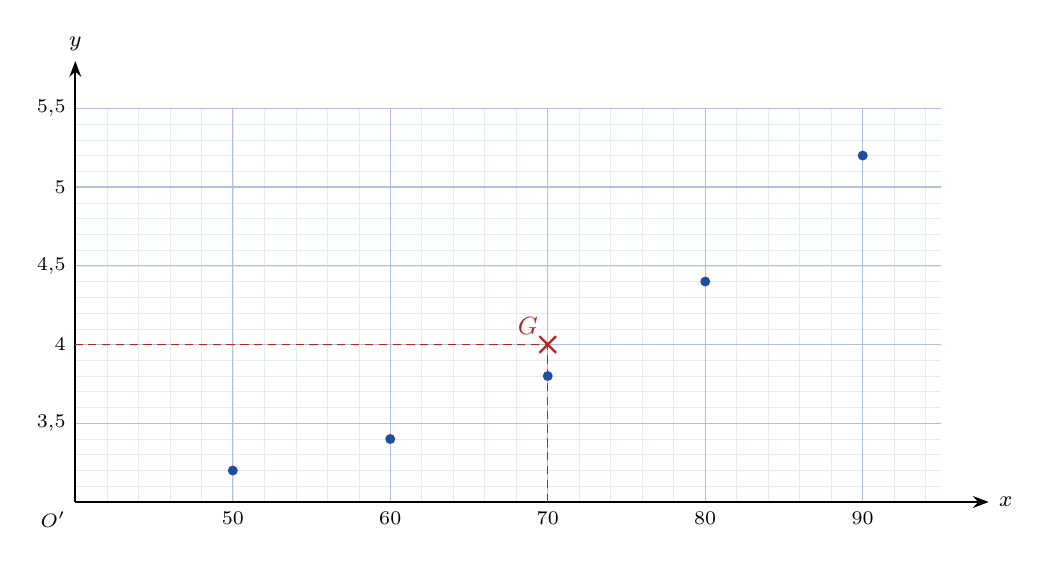
\begin{tikzpicture}[font=\footnotesize]
\draw[cDef!12,very thin](0.000,0)--(0.000,5.000);
\draw[cDef!12,very thin](0.400,0)--(0.400,5.000);
\draw[cDef!12,very thin](0.800,0)--(0.800,5.000);
\draw[cDef!12,very thin](1.200,0)--(1.200,5.000);
\draw[cDef!12,very thin](1.600,0)--(1.600,5.000);
\draw[cDef!12,very thin](2.000,0)--(2.000,5.000);
\draw[cDef!12,very thin](2.400,0)--(2.400,5.000);
\draw[cDef!12,very thin](2.800,0)--(2.800,5.000);
\draw[cDef!12,very thin](3.200,0)--(3.200,5.000);
\draw[cDef!12,very thin](3.600,0)--(3.600,5.000);
\draw[cDef!12,very thin](4.000,0)--(4.000,5.000);
\draw[cDef!12,very thin](4.400,0)--(4.400,5.000);
\draw[cDef!12,very thin](4.800,0)--(4.800,5.000);
\draw[cDef!12,very thin](5.200,0)--(5.200,5.000);
\draw[cDef!12,very thin](5.600,0)--(5.600,5.000);
\draw[cDef!12,very thin](6.000,0)--(6.000,5.000);
\draw[cDef!12,very thin](6.400,0)--(6.400,5.000);
\draw[cDef!12,very thin](6.800,0)--(6.800,5.000);
\draw[cDef!12,very thin](7.200,0)--(7.200,5.000);
\draw[cDef!12,very thin](7.600,0)--(7.600,5.000);
\draw[cDef!12,very thin](8.000,0)--(8.000,5.000);
\draw[cDef!12,very thin](8.400,0)--(8.400,5.000);
\draw[cDef!12,very thin](8.800,0)--(8.800,5.000);
\draw[cDef!12,very thin](9.200,0)--(9.200,5.000);
\draw[cDef!12,very thin](9.600,0)--(9.600,5.000);
\draw[cDef!12,very thin](10.000,0)--(10.000,5.000);
\draw[cDef!12,very thin](10.400,0)--(10.400,5.000);
\draw[cDef!12,very thin](10.800,0)--(10.800,5.000);
\draw[cDef!12,very thin](0,0.000)--(11.000,0.000);
\draw[cDef!12,very thin](0,0.200)--(11.000,0.200);
\draw[cDef!12,very thin](0,0.400)--(11.000,0.400);
\draw[cDef!12,very thin](0,0.600)--(11.000,0.600);
\draw[cDef!12,very thin](0,0.800)--(11.000,0.800);
\draw[cDef!12,very thin](0,1.000)--(11.000,1.000);
\draw[cDef!12,very thin](0,1.200)--(11.000,1.200);
\draw[cDef!12,very thin](0,1.400)--(11.000,1.400);
\draw[cDef!12,very thin](0,1.600)--(11.000,1.600);
\draw[cDef!12,very thin](0,1.800)--(11.000,1.800);
\draw[cDef!12,very thin](0,2.000)--(11.000,2.000);
\draw[cDef!12,very thin](0,2.200)--(11.000,2.200);
\draw[cDef!12,very thin](0,2.400)--(11.000,2.400);
\draw[cDef!12,very thin](0,2.600)--(11.000,2.600);
\draw[cDef!12,very thin](0,2.800)--(11.000,2.800);
\draw[cDef!12,very thin](0,3.000)--(11.000,3.000);
\draw[cDef!12,very thin](0,3.200)--(11.000,3.200);
\draw[cDef!12,very thin](0,3.400)--(11.000,3.400);
\draw[cDef!12,very thin](0,3.600)--(11.000,3.600);
\draw[cDef!12,very thin](0,3.800)--(11.000,3.800);
\draw[cDef!12,very thin](0,4.000)--(11.000,4.000);
\draw[cDef!12,very thin](0,4.200)--(11.000,4.200);
\draw[cDef!12,very thin](0,4.400)--(11.000,4.400);
\draw[cDef!12,very thin](0,4.600)--(11.000,4.600);
\draw[cDef!12,very thin](0,4.800)--(11.000,4.800);
\draw[cDef!12,very thin](0,5.000)--(11.000,5.000);
\draw[cDef!35,thin](0.000,0)--(0.000,5.000);
\draw[cDef!35,thin](2.000,0)--(2.000,5.000);
\draw[cDef!35,thin](4.000,0)--(4.000,5.000);
\draw[cDef!35,thin](6.000,0)--(6.000,5.000);
\draw[cDef!35,thin](8.000,0)--(8.000,5.000);
\draw[cDef!35,thin](10.000,0)--(10.000,5.000);
\draw[cDef!35,thin](0,0.000)--(11.000,0.000);
\draw[cDef!35,thin](0,1.000)--(11.000,1.000);
\draw[cDef!35,thin](0,2.000)--(11.000,2.000);
\draw[cDef!35,thin](0,3.000)--(11.000,3.000);
\draw[cDef!35,thin](0,4.000)--(11.000,4.000);
\draw[cDef!35,thin](0,5.000)--(11.000,5.000);
\draw[-{Stealth[length=2mm]},thick](0,0)--(11.600,0) node[right]{$x$};
\draw[-{Stealth[length=2mm]},thick](0,0)--(0,5.600) node[above]{$y$};
\node[below,font=\scriptsize] at (2.000,0){$50$};
\node[below,font=\scriptsize] at (4.000,0){$60$};
\node[below,font=\scriptsize] at (6.000,0){$70$};
\node[below,font=\scriptsize] at (8.000,0){$80$};
\node[below,font=\scriptsize] at (10.000,0){$90$};
\node[left,font=\scriptsize] at (0,1.000){$3{,}5$};
\node[left,font=\scriptsize] at (0,2.000){$4$};
\node[left,font=\scriptsize] at (0,3.000){$4{,}5$};
\node[left,font=\scriptsize] at (0,4.000){$5$};
\node[left,font=\scriptsize] at (0,5.000){$5{,}5$};
\node[below left,font=\scriptsize] at (0,0){$O'$};
\begin{scope}\clip(0,0) rectangle (11.000,5.000);
\end{scope}
\fill[cDef](2.000,0.400) circle (1.8pt);
\fill[cDef](4.000,0.800) circle (1.8pt);
\fill[cDef](6.000,1.600) circle (1.8pt);
\fill[cDef](8.000,2.800) circle (1.8pt);
\fill[cDef](10.000,4.400) circle (1.8pt);
\draw[cThm,densely dashed](6.000,0)--(6.000,2.000)--(0,2.000);
\draw[cThm,thick](6.000,2.000) +(-3pt,-3pt)--+(3pt,3pt) +(-3pt,3pt)--+(3pt,-3pt);
\node[cThm,above left,font=\small\bfseries] at (6.000,2.000){$G$};
\end{tikzpicture}\end{LTR}\end{center}
(النقطة المتوسطة $G(70;4)$ لأن $\bar x=\frac{350}{5}=70$ و $\bar y=\frac{20}{5}=4$.)

\QQ{2} من أجل $x=130$: $y=0{,}05\times130+0{,}5=6{,}5+0{,}5=7$.

الاستهلاك المقدّر بالتعديل الخطي: \bx{7\ l/100km}.

\QQ{3}
\pa
\begin{center}\begin{LTR}\renewcommand{\arraystretch}{1.25}
\begin{tabular}{|>{\columncolor{cSec!6}}c|*{5}{c|}}\hline
\rowcolor{cSec!12}$x_i$ & 50 & 60 & 70 & 80 & 90\\\hline
$y_i$ & $3{,}2$ & $3{,}4$ & $3{,}8$ & $4{,}4$ & $5{,}2$\\\hline
$z_i=\ln y_i$ & $1{,}16$ & $1{,}22$ & $1{,}34$ & $1{,}48$ & $1{,}65$\\\hline
\end{tabular}\end{LTR}\end{center}
\pb \[\bar x=\frac{350}{5}=70\qquad \bar z=\frac{1{,}16+1{,}22+1{,}34+1{,}48+1{,}65}{5}=\frac{6{,}85}{5}=1{,}37\]
إذن \bx{(\bar x;\bar z)=(70\,;\,1{,}37)}.
\pc جدول الحساب:
\begin{center}\begin{LTR}\renewcommand{\arraystretch}{1.25}
\begin{tabular}{|>{\columncolor{cSec!6}}c|*{5}{c|}>{\columncolor{cEx!10}}c|}\hline
\rowcolor{cSec!12}$x_i$ & 50 & 60 & 70 & 80 & 90 & $350$\\\hline
$z_i$ & $1{,}16$ & $1{,}22$ & $1{,}34$ & $1{,}48$ & $1{,}65$ & $6{,}85$\\\hline
$x_i^2$ & 2500 & 3600 & 4900 & 6400 & 8100 & $25500$\\\hline
$x_iz_i$ & $58$ & $73{,}2$ & $93{,}8$ & $118{,}4$ & $148{,}5$ & $491{,}9$\\\hline
\end{tabular}\end{LTR}\end{center}
\[V(x)=\frac{25500}{5}-70^{2}=5100-4900=200\]
\[\operatorname{cov}(x,z)=\frac{491{,}9}{5}-70\times1{,}37=98{,}38-95{,}9=2{,}48\]
\[a=\frac{2{,}48}{200}=0{,}0124\]
\[b=\bar z-a\bar x=1{,}37-0{,}0124\times70=1{,}37-0{,}868=0{,}502\]
\[\bx{z=0{,}0124x+0{,}502}\]
\begin{molahada}
التدوير إلى $10^{-2}$ يخص ملء الجدول فقط؛ لو دوّرنا $a$ إلى $10^{-2}$ لصار $0{,}01$ وفقدنا الدقة، لذا نحتفظ بـ $a=0{,}0124$ و $b=0{,}502$.
\end{molahada}
\pd $z=\ln y$ يعني $y=e^{z}=e^{0{,}0124x+0{,}502}=e^{0{,}502}\,e^{0{,}0124x}$، أي:
\[\bx{y\approx1{,}65\,e^{0{,}0124x}}\]
من أجل $x=130$: $y=e^{0{,}0124\times130+0{,}502}=e^{2{,}114}\approx8{,}28$.

الاستهلاك المقدّر بهذا التعديل: \bx{8{,}28\ l/100km} تقريبا.
\pe من $90$ إلى $130\,km/h$ تزداد السرعة $4$ مرات بـ $10\,km/h$، فالاستهلاك الحقيقي:
\[5{,}2+4\times0{,}75=5{,}2+3=8{,}2\ l/100km\]
\begin{itemize}
\item التعديل الخطي: $|7-8{,}2|=1{,}2$.
\item التعديل الأسّي: $|8{,}28-8{,}2|=0{,}08$.
\end{itemize}
إذن \bxt{التعديل الأسّي $y\approx1{,}65\,e^{0{,}0124x}$ يعطي أفضل تقدير}.
\end{hal}
% ===================== بكالوريا 2016 -- الموضوع الثاني =====================
\Needspace{16\baselineskip}
\begin{tamrin}{بكالوريا 2016 -- الموضوع الثاني -- تسيير واقتصاد}
الجدول التالي يبيّن كمية الإنتاج السنوي بآلاف الأطنان من البطاطا لتعاونية فلاحية ما بين سنتي $2010$ و $2015$.
\begin{center}
\begin{tabular}{|C|c|c|c|c|c|c|}\hline
\rowcolor{cSec!12} السنة & $2010$ & $2011$ & $2012$ & $2013$ & $2014$ & $2015$\\\hline
رتبة السنة $x_i$ & $1$ & $2$ & $3$ & $4$ & $5$ & $6$\\\hline
كمية المنتوج بآلاف الأطنان $y_i$ & $25$ & $30$ & $33$ & $42$ & $48$ & $55$\\\hline
\end{tabular}
\end{center}

\QQ{1} مثّل سحابة النقط $M_i(x_i;y_i)$ في معلم متعامد ومتجانس حيث على محور الفواصل كل $1\,\text{cm}$ تمثل سنة واحدة، وعلى محور التراتيب كل $1\,\text{cm}$ يمثل $10$ آلاف طن.
\QQ{2} عيّن إحداثيي النقطة المتوسطة $G$ ثم علّمها.
\QQ{3}
\begin{sq}
\qa اكتب معادلة من الشكل $y=ax+b$ لمستقيم الانحدار بالمربعات الدنيا. (تدوّر $a$ و $b$ إلى $10^{-2}$)
\qb أنشئ المستقيم $(\Delta)$.
\end{sq}
\QQ{4} باستعمال هذا التعديل:
\begin{itemize}
\item احسب كمية إنتاج التعاونية سنة $2020$.
\item في أي سنة يتجاوز الإنتاج $20$ ألف طن؟
\end{itemize}
\end{tamrin}

\Needspace{13cm}
\begin{hal}
\QQ{1} نأخذ على محور الفواصل $1\,\text{cm}$ لكل سنة، وعلى محور التراتيب $1\,\text{cm}$ لكل $10$ آلاف طن، فالنقطة $M_i$ ترتيبها على الورقة $\dfrac{y_i}{10}\,\text{cm}$. سحابة النقط (بالبرتقالي) مع النقطة $G$ والمستقيم $(\Delta)$ المنشأ في السؤال 3:
\begin{center}\begin{LTR}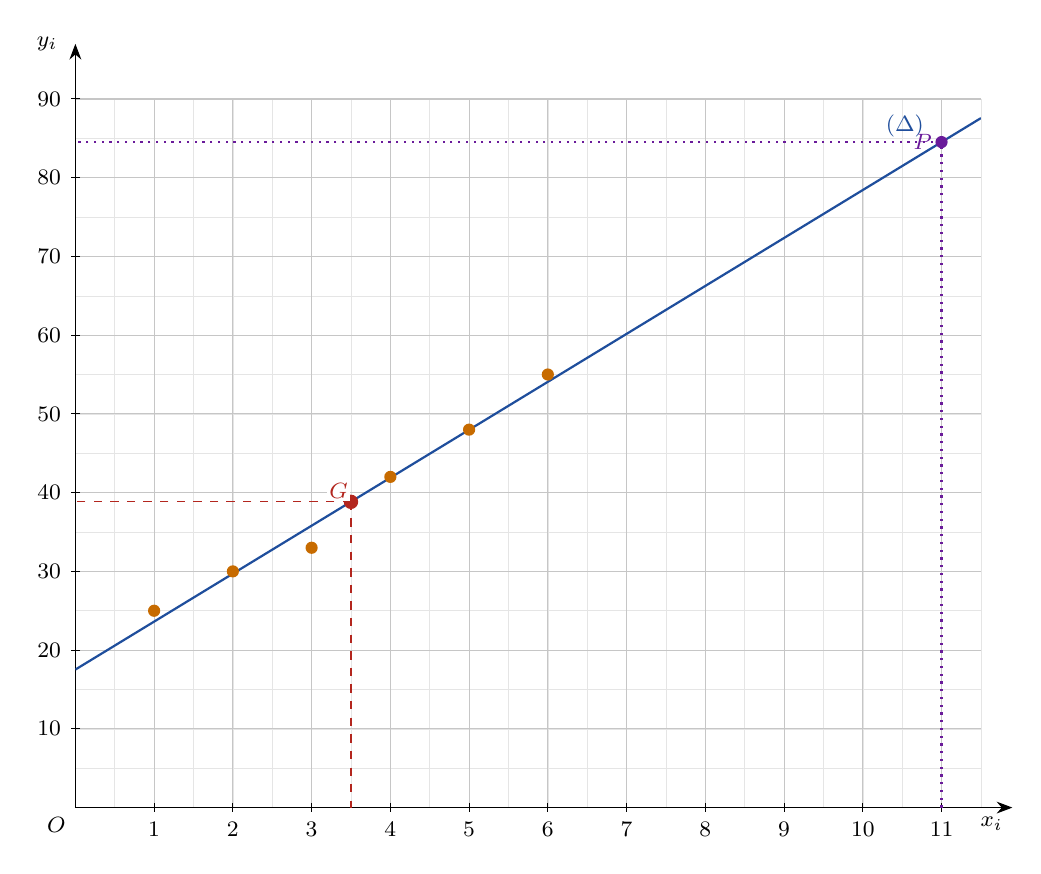
\begin{tikzpicture}[x=1cm,y=1cm,font=\footnotesize]
\draw[gray!20,very thin,step=0.5] (0,0) grid (11.500,9.000);
\draw[gray!45,thin,step=1] (0,0) grid (11.500,9.000);
\draw[-{Stealth[length=2mm]}] (0,0)--(11.900,0) node[below left]{$x_i$};
\draw[-{Stealth[length=2mm]}] (0,0)--(0,9.700) node[left=3pt]{$y_i$};
\node[below left] at (0,0){$O$};
\draw (1.000,0.06)--(1.000,-0.06) node[below]{$1$};
\draw (2.000,0.06)--(2.000,-0.06) node[below]{$2$};
\draw (3.000,0.06)--(3.000,-0.06) node[below]{$3$};
\draw (4.000,0.06)--(4.000,-0.06) node[below]{$4$};
\draw (5.000,0.06)--(5.000,-0.06) node[below]{$5$};
\draw (6.000,0.06)--(6.000,-0.06) node[below]{$6$};
\draw (7.000,0.06)--(7.000,-0.06) node[below]{$7$};
\draw (8.000,0.06)--(8.000,-0.06) node[below]{$8$};
\draw (9.000,0.06)--(9.000,-0.06) node[below]{$9$};
\draw (10.000,0.06)--(10.000,-0.06) node[below]{$10$};
\draw (11.000,0.06)--(11.000,-0.06) node[below]{$11$};
\draw (0.06,1.000)--(-0.06,1.000) node[left]{$10$};
\draw (0.06,2.000)--(-0.06,2.000) node[left]{$20$};
\draw (0.06,3.000)--(-0.06,3.000) node[left]{$30$};
\draw (0.06,4.000)--(-0.06,4.000) node[left]{$40$};
\draw (0.06,5.000)--(-0.06,5.000) node[left]{$50$};
\draw (0.06,6.000)--(-0.06,6.000) node[left]{$60$};
\draw (0.06,7.000)--(-0.06,7.000) node[left]{$70$};
\draw (0.06,8.000)--(-0.06,8.000) node[left]{$80$};
\draw (0.06,9.000)--(-0.06,9.000) node[left]{$90$};
\begin{scope}\clip (0,0.000) rectangle (11.500,9.000);
\draw[cDef,thick,domain=0:11.500,samples=2] plot (\x*1.0000,{0.000000+(6.090000*\x+17.530000-0.000000)/10.000000});
\end{scope}
\node[cDef,above left] at (10.900,8.391){$(\Delta)$};
\fill[cEx] (1.000,2.500) circle (2.2pt);
\fill[cEx] (2.000,3.000) circle (2.2pt);
\fill[cEx] (3.000,3.300) circle (2.2pt);
\fill[cEx] (4.000,4.200) circle (2.2pt);
\fill[cEx] (5.000,4.800) circle (2.2pt);
\fill[cEx] (6.000,5.500) circle (2.2pt);
\draw[cThm,dashed] (3.500,3.883)--(3.500,0) (3.500,3.883)--(0,3.883);
\fill[cThm] (3.500,3.883) circle (2.6pt) node[above left,fill=white,inner sep=1pt]{$G$};
\fill[cMeth] (11,8.452) circle (2.2pt) node[left]{$P$};
\draw[cMeth,dotted,thick] (11,0)--(11,8.452)--(0,8.452);
\end{tikzpicture}\end{LTR}\end{center}

\QQ{2}
\[\bar x=\dfrac{1+2+3+4+5+6}{6}=\dfrac{21}{6}=3{,}5\]
\[\bar y=\dfrac{25+30+33+42+48+55}{6}=\dfrac{233}{6}\approx38{,}83\]
\[\bx{G\left(3{,}5\,;\,\tfrac{233}{6}\right)\approx G(3{,}5\,;\,38{,}83)}\]
\QQ{3}
\pa جدول الحسابات:
\begin{center}\small
\begin{tabular}{|C|c|c|c|c|c|c|C|}\hline
\rowcolor{cSec!12} $i$ & $1$ & $2$ & $3$ & $4$ & $5$ & $6$ & المجموع\\\hline
$x_i$ & $1$ & $2$ & $3$ & $4$ & $5$ & $6$ & $21$\\\hline
$y_i$ & $25$ & $30$ & $33$ & $42$ & $48$ & $55$ & $233$\\\hline
$x_i^{2}$ & $1$ & $4$ & $9$ & $16$ & $25$ & $36$ & $91$\\\hline
$x_iy_i$ & $25$ & $60$ & $99$ & $168$ & $240$ & $330$ & $922$\\\hline
\end{tabular}
\end{center}
\textbf{التباين:}
\[V(x)=\frac1{6}\sum x_i^{2}-\bar x^{2}=\frac{91}{6}-(3{,}5)^{2}=\frac{35}{12}\approx 2{,}9167\]
\textbf{التغاير:}
\[\operatorname{cov}(x,y)=\frac1{6}\sum x_iy_i-\bar x\,\bar y=\frac{\sum x_iy_i-\bar x\sum y_i}{6}=\frac{922-3{,}5\times233}{6}=\frac{106{,}5}{6}=17{,}75\]

ومنه:
\[a=\frac{\operatorname{cov}(x,y)}{V(x)}=\frac{17{,}75}{35/12}=\frac{213}{35}\approx6{,}0857\approx6{,}09\]
\[b=\bar y-a\,\bar x=\frac{233}{6}-\frac{213}{35}\times3{,}5\approx38{,}8333-21{,}3000=17{,}5333\approx17{,}53\]
\[\bx{(\Delta):\ y=6{,}09\,x+17{,}53}\]
\pb $(\Delta)$ يشمل النقطة $G$؛ ونأخذ نقطة ثانية، مثلا من أجل $x=0$: $y=17{,}53$، أي النقطة $(0\,;17{,}53)$. (انظر الشكل أعلاه.)
\QQ{4}
\begin{itemize}
\item سنة $2020$ رتبتها $x=2020-2009=11$:
\[y=6{,}09\times11+17{,}53=66{,}99+17{,}53=84{,}52\]
\bxt{تقدير إنتاج سنة $2020$ هو حوالي $84{,}52$ ألف طن} (النقطة $P$ على الشكل).
\item نحل المتراجحة $y>20$:
\[6{,}09\,x+17{,}53>20\iff x>\frac{20-17{,}53}{6{,}09}=\frac{2{,}47}{6{,}09}\approx0{,}41\]
وكل الرتب $x\geqslant1$ تحققها، أي أن الإنتاج يتجاوز $20$ ألف طن \textbf{منذ السنة الأولى $2010$} (وهو ما يؤكده الجدول: $y_1=25>20$).
\end{itemize}
\end{hal}
\begin{molahada}
السؤال الأخير كما ورد (عتبة $20$ ألف طن) بديهي لأن الإنتاج يفوق $20$ ألف طن منذ $2010$؛ يبدو أن العتبة المقصودة أكبر. مثلا لعتبة $100$ ألف طن: $6{,}09x+17{,}53>100\iff x>\dfrac{82{,}47}{6{,}09}\approx13{,}54$، أي $x=14$ وهي سنة $2009+14=2023$.
\end{molahada}

% ===================== بكالوريا 2017 -- الموضوع الأول =====================
\Needspace{16\baselineskip}
\begin{tamrin}{بكالوريا 2017 -- الموضوع الأول -- تسيير واقتصاد}
الجدول التالي يمثل تطور ميزانية الإشهار بالمليون دينار لمؤسسة اقتصادية من سنة $2009$ إلى سنة $2016$.
\begin{center}
\begin{tabular}{|C|c|c|c|c|c|c|c|c|}\hline
\rowcolor{cSec!12} السنة & $2009$ & $2010$ & $2011$ & $2012$ & $2013$ & $2014$ & $2015$ & $2016$\\\hline
ترتيب السنوات $x_i$ & $1$ & $2$ & $3$ & $4$ & $5$ & $6$ & $7$ & $8$\\\hline
الميزانية $y_i$ بالمليون دينار & $0{,}4$ & $0{,}45$ & $0{,}5$ & $0{,}56$ & $0{,}63$ & $0{,}68$ & $0{,}75$ & $0{,}83$\\\hline
\end{tabular}
\end{center}

\QQ{1} مثّل سحابة النقط $M_i(x_i;y_i)$ في معلم متعامد.\\
(نأخذ $1\,\text{cm}$ لكل سنة على محور الفواصل و $1\,\text{cm}$ لكل $100\,000\,\text{DA}$ على محور التراتيب)
\QQ{2} جد إحداثيي النقطة المتوسطة $G$ لسحابة النقط ثم علّمها.
\QQ{3} بيّن أن معادلة مستقيم الانحدار $(\Delta)$ بالمربعات الدنيا هي: $y=0{,}06x+0{,}33$ (النتائج تدوّر إلى $10^{-2}$)، ثم ارسم المستقيم $(\Delta)$ في المعلم السابق.
\QQ{4}
\begin{sq}
\qa باستعمال التعديل الخطي السابق قدّر الميزانية المتوقعة سنة $2020$.
\qb ابتداءً من أي سنة تتجاوز هذه الميزانية $1\,200\,000\,\text{DA}$؟
\end{sq}
\end{tamrin}
\Needspace{14.5cm}
\begin{hal}
\QQ{1} $y_i$ مقدّرة بالمليون دينار، و $100\,000\,\text{DA}=0{,}1$ مليون دينار، فكل $1\,\text{cm}$ على محور التراتيب يمثل $0{,}1$ مليون دينار، أي أن ترتيب $M_i$ على الورقة هو $10\,y_i$ cm (مثلا $M_8$ على ارتفاع $8{,}3\,\text{cm}$).
\begin{center}\begin{LTR}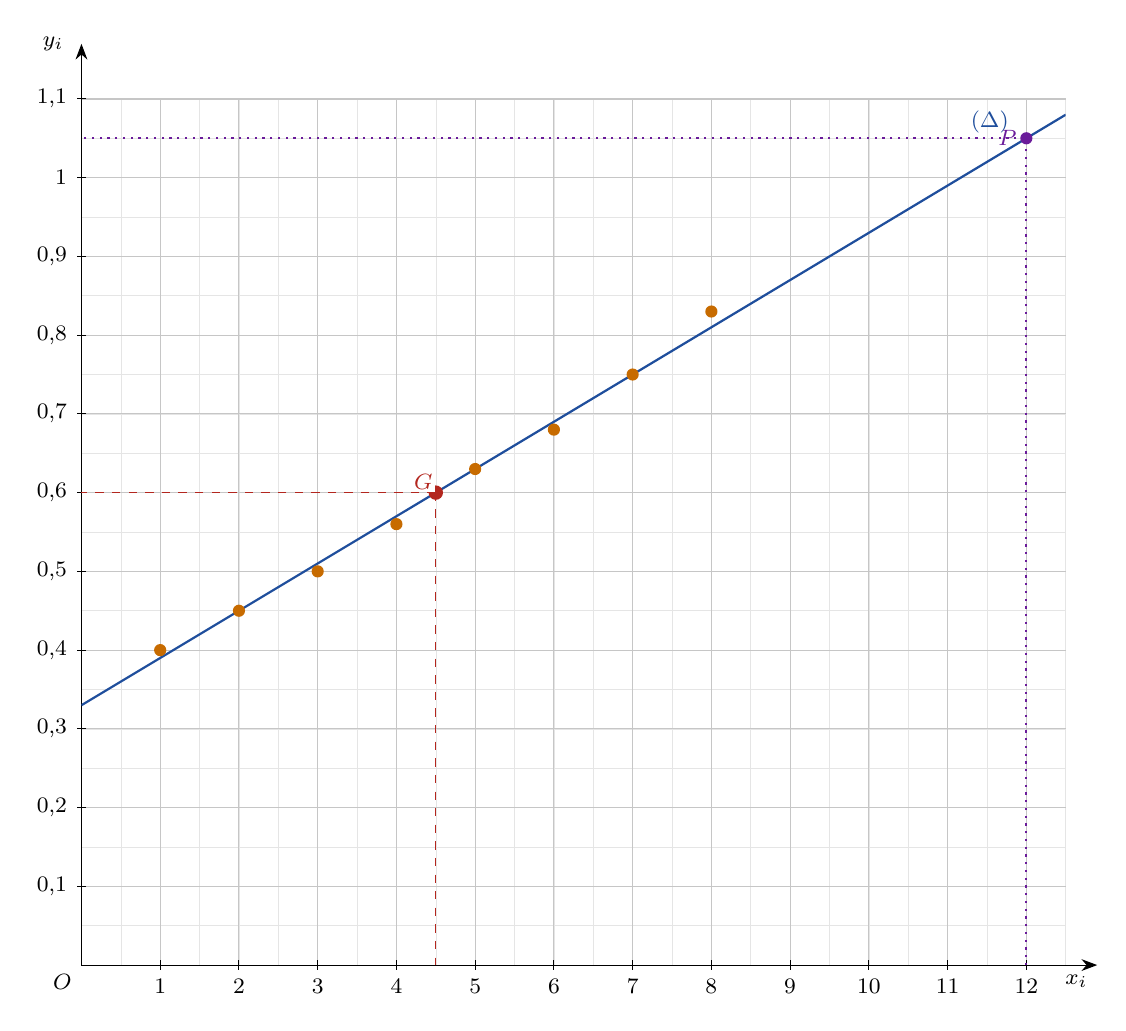
\begin{tikzpicture}[x=1cm,y=1cm,font=\footnotesize]
\draw[gray!20,very thin,step=0.5] (0,0) grid (12.500,11.000);
\draw[gray!45,thin,step=1] (0,0) grid (12.500,11.000);
\draw[-{Stealth[length=2mm]}] (0,0)--(12.900,0) node[below left]{$x_i$};
\draw[-{Stealth[length=2mm]}] (0,0)--(0,11.700) node[left=3pt]{$y_i$};
\node[below left] at (0,0){$O$};
\draw (1.000,0.06)--(1.000,-0.06) node[below]{$1$};
\draw (2.000,0.06)--(2.000,-0.06) node[below]{$2$};
\draw (3.000,0.06)--(3.000,-0.06) node[below]{$3$};
\draw (4.000,0.06)--(4.000,-0.06) node[below]{$4$};
\draw (5.000,0.06)--(5.000,-0.06) node[below]{$5$};
\draw (6.000,0.06)--(6.000,-0.06) node[below]{$6$};
\draw (7.000,0.06)--(7.000,-0.06) node[below]{$7$};
\draw (8.000,0.06)--(8.000,-0.06) node[below]{$8$};
\draw (9.000,0.06)--(9.000,-0.06) node[below]{$9$};
\draw (10.000,0.06)--(10.000,-0.06) node[below]{$10$};
\draw (11.000,0.06)--(11.000,-0.06) node[below]{$11$};
\draw (12.000,0.06)--(12.000,-0.06) node[below]{$12$};
\draw (0.06,1.000)--(-0.06,1.000) node[left]{$0{,}1$};
\draw (0.06,2.000)--(-0.06,2.000) node[left]{$0{,}2$};
\draw (0.06,3.000)--(-0.06,3.000) node[left]{$0{,}3$};
\draw (0.06,4.000)--(-0.06,4.000) node[left]{$0{,}4$};
\draw (0.06,5.000)--(-0.06,5.000) node[left]{$0{,}5$};
\draw (0.06,6.000)--(-0.06,6.000) node[left]{$0{,}6$};
\draw (0.06,7.000)--(-0.06,7.000) node[left]{$0{,}7$};
\draw (0.06,8.000)--(-0.06,8.000) node[left]{$0{,}8$};
\draw (0.06,9.000)--(-0.06,9.000) node[left]{$0{,}9$};
\draw (0.06,10.000)--(-0.06,10.000) node[left]{$1$};
\draw (0.06,11.000)--(-0.06,11.000) node[left]{$1{,}1$};
\begin{scope}\clip (0,0.000) rectangle (12.500,11.000);
\draw[cDef,thick,domain=0:12.500,samples=2] plot (\x*1.0000,{0.000000+(0.060000*\x+0.330000-0.000000)/0.100000});
\end{scope}
\node[cDef,above left] at (11.900,10.440){$(\Delta)$};
\fill[cEx] (1.000,4.000) circle (2.2pt);
\fill[cEx] (2.000,4.500) circle (2.2pt);
\fill[cEx] (3.000,5.000) circle (2.2pt);
\fill[cEx] (4.000,5.600) circle (2.2pt);
\fill[cEx] (5.000,6.300) circle (2.2pt);
\fill[cEx] (6.000,6.800) circle (2.2pt);
\fill[cEx] (7.000,7.500) circle (2.2pt);
\fill[cEx] (8.000,8.300) circle (2.2pt);
\draw[cThm,dashed] (4.500,6.000)--(4.500,0) (4.500,6.000)--(0,6.000);
\fill[cThm] (4.500,6.000) circle (2.6pt) node[above left,fill=white,inner sep=1pt]{$G$};
\fill[cMeth] (12,10.5) circle (2.2pt) node[left]{$P$};
\draw[cMeth,dotted,thick] (12,0)--(12,10.5)--(0,10.5);
\end{tikzpicture}\end{LTR}\end{center}

\QQ{2}
\[\bar x=\dfrac{1+2+\dots+8}{8}=\dfrac{36}{8}=4{,}5\]
\[\bar y=\dfrac{0{,}4+0{,}45+0{,}5+0{,}56+0{,}63+0{,}68+0{,}75+0{,}83}{8}=\dfrac{4{,}8}{8}=0{,}6\]
\[\bx{G(4{,}5\,;\,0{,}6)}\]
\QQ{3} جدول الحسابات:
\begin{center}\small
\begin{tabular}{|C|c|c|c|c|c|c|c|c|C|}\hline
\rowcolor{cSec!12} $i$ & $1$ & $2$ & $3$ & $4$ & $5$ & $6$ & $7$ & $8$ & المجموع\\\hline
$x_i$ & $1$ & $2$ & $3$ & $4$ & $5$ & $6$ & $7$ & $8$ & $36$\\\hline
$y_i$ & $0{,}4$ & $0{,}45$ & $0{,}5$ & $0{,}56$ & $0{,}63$ & $0{,}68$ & $0{,}75$ & $0{,}83$ & $4{,}8$\\\hline
$x_i^{2}$ & $1$ & $4$ & $9$ & $16$ & $25$ & $36$ & $49$ & $64$ & $204$\\\hline
$x_iy_i$ & $0{,}4$ & $0{,}9$ & $1{,}5$ & $2{,}24$ & $3{,}15$ & $4{,}08$ & $5{,}25$ & $6{,}64$ & $24{,}16$\\\hline
\end{tabular}
\end{center}
\textbf{التباين:}
\[V(x)=\frac1{8}\sum x_i^{2}-\bar x^{2}=\frac{204}{8}-(4{,}5)^{2}=5{,}25\]
\textbf{التغاير:}
\[\operatorname{cov}(x,y)=\frac1{8}\sum x_iy_i-\bar x\,\bar y=\frac{\sum x_iy_i-\bar x\sum y_i}{8}=\frac{24{,}16-4{,}5\times4{,}8}{8}=\frac{2{,}56}{8}=0{,}32\]

\[a=\frac{\operatorname{cov}(x,y)}{V(x)}=\frac{0{,}32}{5{,}25}\approx0{,}061\approx0{,}06\]
\[b=\bar y-a\bar x=0{,}6-\frac{0{,}32}{5{,}25}\times4{,}5\approx0{,}6-0{,}274=0{,}326\approx0{,}33\]
\[\bx{(\Delta):\ y=0{,}06\,x+0{,}33}\]
وهي المعادلة المطلوبة. لرسم $(\Delta)$: يشمل $G(4{,}5;0{,}6)$ والنقطة $(0;0{,}33)$ (أو $(8;0{,}81)$).
\QQ{4}
\pa سنة $2020$ رتبتها $x=2020-2008=12$:
\[y=0{,}06\times12+0{,}33=0{,}72+0{,}33=1{,}05\]
\bxt{الميزانية المتوقعة سنة $2020$ حوالي $1{,}05$ مليون دينار، أي $1\,050\,000\,\text{DA}$}.
\pb $1\,200\,000\,\text{DA}=1{,}2$ مليون دينار:
\[0{,}06\,x+0{,}33>1{,}2\iff 0{,}06\,x>0{,}87\iff x>\frac{0{,}87}{0{,}06}=14{,}5\]
أصغر رتبة صحيحة هي $x=15$، وهي سنة $2008+15=2023$: \bxt{تتجاوز الميزانية $1\,200\,000\,\text{DA}$ ابتداءً من سنة $2023$}.
\end{hal}

% ===================== بكالوريا 2017 -- الموضوع الثاني =====================
\Needspace{16\baselineskip}
\begin{tamrin}{بكالوريا 2017 -- الموضوع الثاني -- تسيير واقتصاد}
يمثل الجدول التالي نسب النجاح في امتحان شهادة البكالوريا لشعبة التسيير والاقتصاد بثانوية في الفترة من سنة $2010$ إلى $2014$.
\begin{center}
\begin{tabular}{|C|c|c|c|c|c|}\hline
\rowcolor{cSec!12} السنة & $2010$ & $2011$ & $2012$ & $2013$ & $2014$\\\hline
رتبة السنة $x_i$ & $1$ & $2$ & $3$ & $4$ & $5$\\\hline
النسبة المئوية $y_i$ & $33{,}1$ & $36{,}8$ & $41$ & $41{,}1$ & $44{,}1$\\\hline
$z_i=\ln y_i$ &  &  &  &  & \\\hline
\end{tabular}
\end{center}

\QQ{1} عيّن إحداثيي $G$ النقطة المتوسطة لسحابة النقط $M_i(x_i;y_i)$.
\QQ{2} لتكن $y=ax+b$ معادلة مستقيم الانحدار بالمربعات الدنيا للسلسلة $(x_i;y_i)$. بيّن أن $a=2{,}63$ ثم احسب قيمة $b$.
\QQ{3}
\begin{sq}
\qa أكمل السطر الأخير من الجدول أعلاه. (تدوّر النتائج إلى $10^{-2}$)
\qb بيّن أن معادلة مستقيم الانحدار بالمربعات الدنيا للسلسلة $(x_i;z_i)$ هي: $z=0{,}07x+3{,}46$.
\end{sq}
\QQ{4} من بين التعديلين السابقين، ما هو التعديل الذي يعطي أكبر نسبة نجاح في سنة $2017$؟
\end{tamrin}
\Needspace{14cm}
\begin{hal}
\QQ{1}
\[\bar x=\dfrac{1+2+3+4+5}{5}=3\]
\[\bar y=\dfrac{33{,}1+36{,}8+41+41{,}1+44{,}1}{5}=\dfrac{196{,}1}{5}=39{,}22\]
\[\bx{G(3\,;\,39{,}22)}\]
للتوضيح (السؤال لا يطلب ذلك)، سحابة النقط مع $G$ والمستقيم (من السؤال 2) في معلم متعامد: $1\,\text{cm}$ لكل سنة و $1\,\text{cm}$ لكل $2\%$ على محور التراتيب، بدءًا من $32\%$ (المحور مقطوع):
\begin{center}\begin{LTR}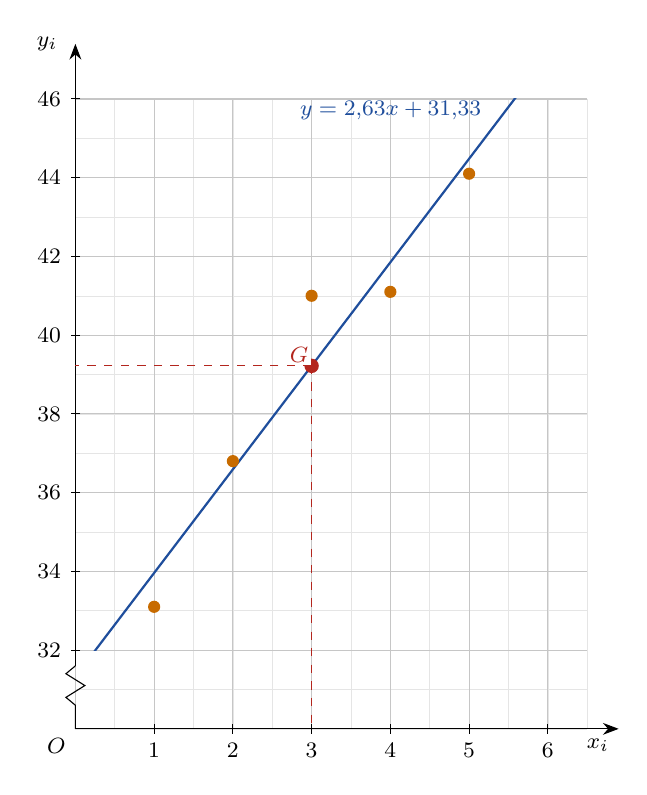
\begin{tikzpicture}[x=1cm,y=1cm,font=\footnotesize]
\draw[gray!20,very thin,step=0.5] (0,0) grid (6.500,8.000);
\draw[gray!45,thin,step=1] (0,0) grid (6.500,8.000);
\draw[-{Stealth[length=2mm]}] (0,0)--(6.900,0) node[below left]{$x_i$};
\draw (0,0)--(0,0.3)--(-0.12,0.4)--(0.12,0.55)--(-0.12,0.7)--(0,0.8);
\draw[-{Stealth[length=2mm]}] (0,0.8)--(0,8.700) node[left=3pt]{$y_i$};
\node[below left] at (0,0){$O$};
\draw (1.000,0.06)--(1.000,-0.06) node[below]{$1$};
\draw (2.000,0.06)--(2.000,-0.06) node[below]{$2$};
\draw (3.000,0.06)--(3.000,-0.06) node[below]{$3$};
\draw (4.000,0.06)--(4.000,-0.06) node[below]{$4$};
\draw (5.000,0.06)--(5.000,-0.06) node[below]{$5$};
\draw (6.000,0.06)--(6.000,-0.06) node[below]{$6$};
\draw (0.06,1.000)--(-0.06,1.000) node[left]{$32$};
\draw (0.06,2.000)--(-0.06,2.000) node[left]{$34$};
\draw (0.06,3.000)--(-0.06,3.000) node[left]{$36$};
\draw (0.06,4.000)--(-0.06,4.000) node[left]{$38$};
\draw (0.06,5.000)--(-0.06,5.000) node[left]{$40$};
\draw (0.06,6.000)--(-0.06,6.000) node[left]{$42$};
\draw (0.06,7.000)--(-0.06,7.000) node[left]{$44$};
\draw (0.06,8.000)--(-0.06,8.000) node[left]{$46$};
\begin{scope}\clip (0,1.000) rectangle (6.500,8.000);
\draw[cDef,thick,domain=0:6.500,samples=2] plot (\x*1.0000,{1.000000+(2.630000*\x+31.330000-32.000000)/2.000000});
\end{scope}
\node[cDef,above left] at (5.278,7.605){$y=2{,}63x+31{,}33$};
\fill[cEx] (1.000,1.550) circle (2.2pt);
\fill[cEx] (2.000,3.400) circle (2.2pt);
\fill[cEx] (3.000,5.500) circle (2.2pt);
\fill[cEx] (4.000,5.550) circle (2.2pt);
\fill[cEx] (5.000,7.050) circle (2.2pt);
\draw[cThm,dashed] (3.000,4.610)--(3.000,0) (3.000,4.610)--(0,4.610);
\fill[cThm] (3.000,4.610) circle (2.6pt) node[above left,fill=white,inner sep=1pt]{$G$};
\end{tikzpicture}\end{LTR}\end{center}

\QQ{2} جدول الحسابات:
\begin{center}\small
\begin{tabular}{|C|c|c|c|c|c|C|}\hline
\rowcolor{cSec!12} $i$ & $1$ & $2$ & $3$ & $4$ & $5$ & المجموع\\\hline
$x_i$ & $1$ & $2$ & $3$ & $4$ & $5$ & $15$\\\hline
$y_i$ & $33{,}1$ & $36{,}8$ & $41$ & $41{,}1$ & $44{,}1$ & $196{,}1$\\\hline
$x_i^{2}$ & $1$ & $4$ & $9$ & $16$ & $25$ & $55$\\\hline
$x_iy_i$ & $33{,}1$ & $73{,}6$ & $123$ & $164{,}4$ & $220{,}5$ & $614{,}6$\\\hline
\end{tabular}
\end{center}
\textbf{التباين:}
\[V(x)=\frac1{5}\sum x_i^{2}-\bar x^{2}=\frac{55}{5}-3^{2}=2\]
\textbf{التغاير:}
\[\operatorname{cov}(x,y)=\frac1{5}\sum x_iy_i-\bar x\,\bar y=\frac{\sum x_iy_i-\bar x\sum y_i}{5}=\frac{614{,}6-3\times196{,}1}{5}=\frac{26{,}3}{5}=5{,}26\]

\[a=\frac{\operatorname{cov}(x,y)}{V(x)}=\frac{5{,}26}{2}=2{,}63\]
\[b=\bar y-a\bar x=39{,}22-2{,}63\times3=39{,}22-7{,}89=31{,}33\]
\[\bx{a=2{,}63}\qquad \bx{b=31{,}33}\qquad\text{أي}\qquad \bx{y=2{,}63\,x+31{,}33}\]

\QQ{3}
\pa بالآلة الحاسبة: $\ln33{,}1\approx3{,}4995$ ، $\ln36{,}8\approx3{,}6055$ ، $\ln41\approx3{,}7136$ ، $\ln41{,}1\approx3{,}7160$ ، $\ln44{,}1\approx3{,}7865$. بالتدوير إلى $10^{-2}$:
\begin{center}
\begin{tabular}{|C|c|c|c|c|c|}\hline
\rowcolor{cSec!12} السنة & $2010$ & $2011$ & $2012$ & $2013$ & $2014$\\\hline
رتبة السنة $x_i$ & $1$ & $2$ & $3$ & $4$ & $5$\\\hline
النسبة المئوية $y_i$ & $33{,}1$ & $36{,}8$ & $41$ & $41{,}1$ & $44{,}1$\\\hline
$z_i=\ln y_i$ & $3{,}5$ & $3{,}61$ & $3{,}71$ & $3{,}72$ & $3{,}79$\\\hline
\end{tabular}
\end{center}

\pb نفس الطريقة مع $z_i$ مكان $y_i$:
\begin{center}\small
\begin{tabular}{|C|c|c|c|c|c|C|}\hline
\rowcolor{cSec!12} $i$ & $1$ & $2$ & $3$ & $4$ & $5$ & المجموع\\\hline
$x_i$ & $1$ & $2$ & $3$ & $4$ & $5$ & $15$\\\hline
$z_i$ & $3{,}5$ & $3{,}61$ & $3{,}71$ & $3{,}72$ & $3{,}79$ & $18{,}33$\\\hline
$x_i^{2}$ & $1$ & $4$ & $9$ & $16$ & $25$ & $55$\\\hline
$x_iz_i$ & $3{,}5$ & $7{,}22$ & $11{,}13$ & $14{,}88$ & $18{,}95$ & $55{,}68$\\\hline
\end{tabular}
\end{center}
\textbf{التباين:}
\[V(x)=\frac1{5}\sum x_i^{2}-\bar x^{2}=\frac{55}{5}-3^{2}=2\]
\textbf{التغاير:}
\[\operatorname{cov}(x,z)=\frac1{5}\sum x_iz_i-\bar x\,\bar z=\frac{\sum x_iz_i-\bar x\sum z_i}{5}=\frac{55{,}68-3\times18{,}33}{5}=\frac{0{,}69}{5}=0{,}138\]

$\bar z=\dfrac{18{,}33}{5}=3{,}666$، ومنه:
\[a'=\frac{\operatorname{cov}(x,z)}{V(x)}=\frac{0{,}138}{2}=0{,}069\approx0{,}07\qquad b'=\bar z-a'\bar x=3{,}666-0{,}069\times3=3{,}459\approx3{,}46\]
\[\bx{z=0{,}07\,x+3{,}46}\]
\QQ{4} سنة $2017$ رتبتها $x=2017-2009=8$.
\begin{itemize}
\item \textbf{التعديل الخطي:} $y=2{,}63\times8+31{,}33=21{,}04+31{,}33=52{,}37$، أي حوالي $52{,}37\%$.
\item \textbf{التعديل الأسي:} $z=\ln y$ يعني $y=e^{z}=e^{0{,}07x+3{,}46}$. من أجل $x=8$: $z=0{,}56+3{,}46=4{,}02$، ومنه $y=e^{4{,}02}\approx55{,}70$، أي حوالي $55{,}70\%$.
\end{itemize}
بما أن $55{,}70>52{,}37$: \bxt{التعديل $z=0{,}07x+3{,}46$ (أي $y=e^{0{,}07x+3{,}46}$) يعطي أكبر نسبة نجاح سنة $2017$}.
\end{hal}

% ===================== بكالوريا 2017 -- الدورة الاستثنائية -- الموضوع الأول =====================
\Needspace{16\baselineskip}
\begin{tamrin}{بكالوريا 2017 -- الدورة الاستثنائية -- الموضوع الأول -- تسيير واقتصاد}
الجدول التالي يعطي نسبة الأمية في بلد ما، خلال الفترة الممتدة من $1948$ إلى سنة $2008$.
\begin{center}
\begin{tabular}{|C|c|c|c|c|c|c|c|}\hline
\rowcolor{cSec!12} السنة & $1948$ & $1958$ & $1968$ & $1978$ & $1988$ & $1998$ & $2008$\\\hline
الرتبة $x_i$ & $1$ & $2$ & $3$ & $4$ & $5$ & $6$ & $7$\\\hline
نسبة الأمية $y_i$ & $14$ & $92$ & $74{,}6$ & $60$ & $31$ & $38{,}4$ & $22$\\\hline
\end{tabular}
\end{center}

\QQ{1}
\begin{sq}
\qa احسب إحداثيي النقطة المتوسطة $G$. (تدوّر النتائج إلى $10^{-2}$)
\qb مثّل سحابة النقط $M_i(x_i;y_i)$ في معلم متعامد. (على محور الفواصل $1\,\text{cm}$ يمثل رتبة واحدة، وعلى حامل محور التراتيب $1\,\text{cm}$ يمثل $10\%$)
\end{sq}
\QQ{2} بيّن أن معادلة مستقيم الانحدار بالمربعات الدنيا هي: $y=-4{,}53x+65{,}54$.
\QQ{3} باستعمال التعديل الخطي السابق، قدّر نسبة الأمية في سنة $2038$.
\QQ{4} ابتداءً من أي سنة تكون نسبة الأمية في هذا البلد أقل من $5\%$؟
\end{tamrin}
\Needspace{15cm}
\begin{hal}
\QQ{1}
\pa
\[\bar x=\dfrac{1+2+\dots+7}{7}=\dfrac{28}{7}=4\]
\[\bar y=\dfrac{14+92+74{,}6+60+31+38{,}4+22}{7}=\dfrac{332}{7}\approx47{,}43\]
\[\bx{G(4\,;\,47{,}43)}\]
\pb $1\,\text{cm}$ لكل رتبة و $1\,\text{cm}$ لكل $10\%$ (فالنقطة $M_2(2;92)$ على ارتفاع $9{,}2\,\text{cm}$):
\begin{center}\begin{LTR}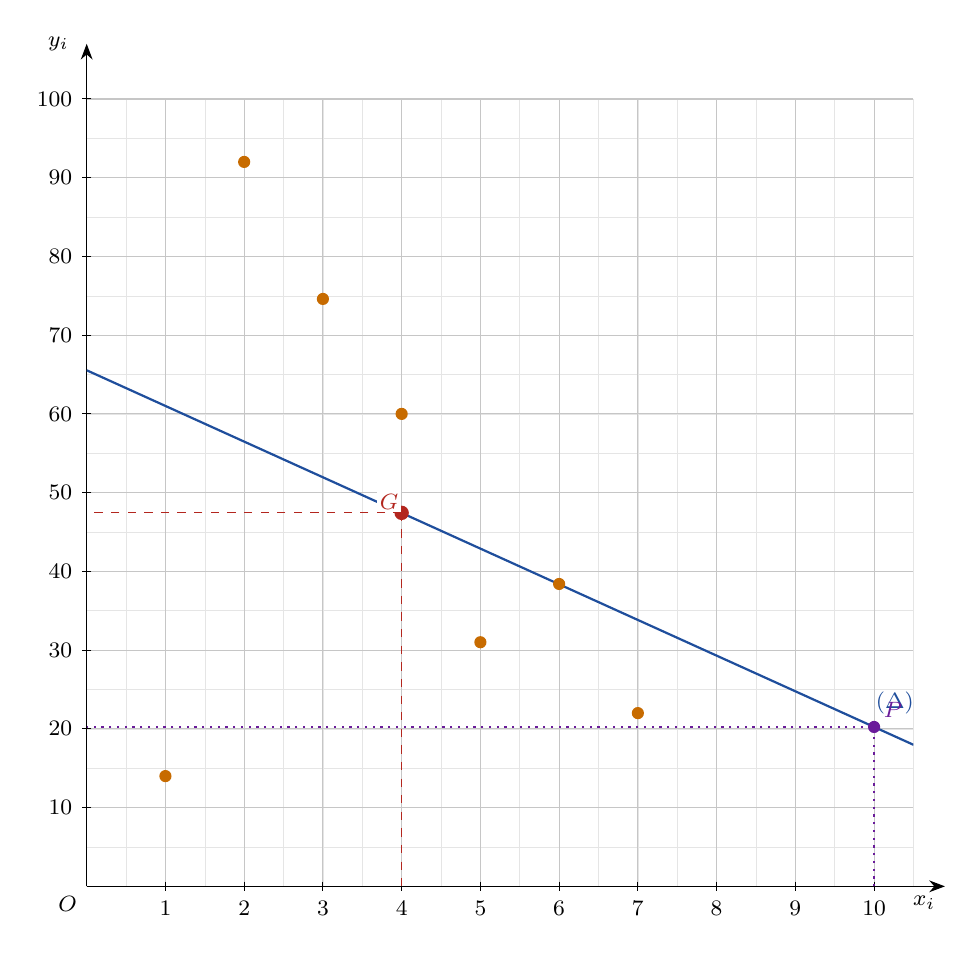
\begin{tikzpicture}[x=1cm,y=1cm,font=\footnotesize]
\draw[gray!20,very thin,step=0.5] (0,0) grid (10.500,10.000);
\draw[gray!45,thin,step=1] (0,0) grid (10.500,10.000);
\draw[-{Stealth[length=2mm]}] (0,0)--(10.900,0) node[below left]{$x_i$};
\draw[-{Stealth[length=2mm]}] (0,0)--(0,10.700) node[left=3pt]{$y_i$};
\node[below left] at (0,0){$O$};
\draw (1.000,0.06)--(1.000,-0.06) node[below]{$1$};
\draw (2.000,0.06)--(2.000,-0.06) node[below]{$2$};
\draw (3.000,0.06)--(3.000,-0.06) node[below]{$3$};
\draw (4.000,0.06)--(4.000,-0.06) node[below]{$4$};
\draw (5.000,0.06)--(5.000,-0.06) node[below]{$5$};
\draw (6.000,0.06)--(6.000,-0.06) node[below]{$6$};
\draw (7.000,0.06)--(7.000,-0.06) node[below]{$7$};
\draw (8.000,0.06)--(8.000,-0.06) node[below]{$8$};
\draw (9.000,0.06)--(9.000,-0.06) node[below]{$9$};
\draw (10.000,0.06)--(10.000,-0.06) node[below]{$10$};
\draw (0.06,1.000)--(-0.06,1.000) node[left]{$10$};
\draw (0.06,2.000)--(-0.06,2.000) node[left]{$20$};
\draw (0.06,3.000)--(-0.06,3.000) node[left]{$30$};
\draw (0.06,4.000)--(-0.06,4.000) node[left]{$40$};
\draw (0.06,5.000)--(-0.06,5.000) node[left]{$50$};
\draw (0.06,6.000)--(-0.06,6.000) node[left]{$60$};
\draw (0.06,7.000)--(-0.06,7.000) node[left]{$70$};
\draw (0.06,8.000)--(-0.06,8.000) node[left]{$80$};
\draw (0.06,9.000)--(-0.06,9.000) node[left]{$90$};
\draw (0.06,10.000)--(-0.06,10.000) node[left]{$100$};
\begin{scope}\clip (0,0.000) rectangle (10.500,10.000);
\draw[cDef,thick,domain=0:10.500,samples=2] plot (\x*1.0000,{0.000000+(-4.530000*\x+65.540000-0.000000)/10.000000});
\end{scope}
\node[cDef,above right] at (9.900,2.069){$(\Delta)$};
\fill[cEx] (1.000,1.400) circle (2.2pt);
\fill[cEx] (2.000,9.200) circle (2.2pt);
\fill[cEx] (3.000,7.460) circle (2.2pt);
\fill[cEx] (4.000,6.000) circle (2.2pt);
\fill[cEx] (5.000,3.100) circle (2.2pt);
\fill[cEx] (6.000,3.840) circle (2.2pt);
\fill[cEx] (7.000,2.200) circle (2.2pt);
\draw[cThm,dashed] (4.000,4.743)--(4.000,0) (4.000,4.743)--(0,4.743);
\fill[cThm] (4.000,4.743) circle (2.6pt) node[above left,fill=white,inner sep=1pt]{$G$};
\fill[cMeth] (10,2.024) circle (2.2pt) node[above right]{$P$};
\draw[cMeth,dotted,thick] (10,0)--(10,2.024)--(0,2.024);
\end{tikzpicture}\end{LTR}\end{center}

\QQ{2} جدول الحسابات:
\begin{center}\small
\begin{tabular}{|C|c|c|c|c|c|c|c|C|}\hline
\rowcolor{cSec!12} $i$ & $1$ & $2$ & $3$ & $4$ & $5$ & $6$ & $7$ & المجموع\\\hline
$x_i$ & $1$ & $2$ & $3$ & $4$ & $5$ & $6$ & $7$ & $28$\\\hline
$y_i$ & $14$ & $92$ & $74{,}6$ & $60$ & $31$ & $38{,}4$ & $22$ & $332$\\\hline
$x_i^{2}$ & $1$ & $4$ & $9$ & $16$ & $25$ & $36$ & $49$ & $140$\\\hline
$x_iy_i$ & $14$ & $184$ & $223{,}8$ & $240$ & $155$ & $230{,}4$ & $154$ & $1201{,}2$\\\hline
\end{tabular}
\end{center}
\textbf{التباين:}
\[V(x)=\frac1{7}\sum x_i^{2}-\bar x^{2}=\frac{140}{7}-4^{2}=4\]
\textbf{التغاير:}
\[\operatorname{cov}(x,y)=\frac1{7}\sum x_iy_i-\bar x\,\bar y=\frac{\sum x_iy_i-\bar x\sum y_i}{7}=\frac{1201{,}2-4\times332}{7}=\frac{-126{,}8}{7}\approx -18{,}1143\]

\[a=\frac{\operatorname{cov}(x,y)}{V(x)}=\frac{-126{,}8/7}{4}=-\frac{126{,}8}{28}\approx-4{,}5286\approx-4{,}53\]
\[b=\bar y-a\bar x=\frac{332}{7}+\frac{126{,}8}{28}\times4=\frac{332+126{,}8}{7}=\frac{458{,}8}{7}\approx65{,}54\]
\[\bx{y=-4{,}53\,x+65{,}54}\]
\QQ{3} الرتب تتقدم بـ $10$ سنوات: الرتبة $x$ توافق السنة $1938+10x$. سنة $2038$ توافق $x=\dfrac{2038-1938}{10}=10$:
\[y=-4{,}53\times10+65{,}54=-45{,}3+65{,}54=20{,}24\]
\bxt{نسبة الأمية المقدّرة سنة $2038$: حوالي $20{,}24\%$} (النقطة $P$ على الشكل).
\QQ{4}
\[-4{,}53\,x+65{,}54<5\iff -4{,}53\,x<-60{,}54\iff x>\frac{60{,}54}{4{,}53}\approx13{,}36\]
(انقلاب الاتجاه لأننا قسمنا على عدد سالب.) السنة الموافقة: $1938+10\times13{,}36\approx2071{,}6$.
\bxt{تصبح نسبة الأمية أقل من $5\%$ ابتداءً من سنة $2072$ تقريبًا}؛ وإن اكتفينا بالرتب الصحيحة (سنة كل عشرية) فأول رتبة هي $x=14$ أي سنة $2078$.
\end{hal}
\begin{molahada}
القيمة $y_1=14$ (سنة $1948$) شاذة عن اتجاه السلسلة المتناقص (ربما المقصود $94$)، لكن المعادلة المعطاة $y=-4{,}53x+65{,}54$ محسوبة فعلا بالقيمة $14$، فاحتفظنا بها. بسبب هذه النقطة تبقى السحابة متباعدة عن المستقيم: معامل الارتباط $r=\dfrac{\operatorname{cov}(x,y)}{\sigma_x\sigma_y}\approx-0{,}34$ ضعيف، فالتقديرات أعلاه تقريبية جدا.
\end{molahada}

% ===================== بكالوريا 2017 -- الدورة الاستثنائية -- الموضوع الثاني =====================
\Needspace{16\baselineskip}
\begin{tamrin}{بكالوريا 2017 -- الدورة الاستثنائية -- الموضوع الثاني -- تسيير واقتصاد}
يمثل الجدول الآتي تطور إنتاج مصنع الإسمنت خلال الفترة الممتدة من $2010$ إلى $2014$.
\begin{center}
\begin{tabular}{|C|c|c|c|c|c|}\hline
\rowcolor{cSec!12} السنة & $2010$ & $2011$ & $2012$ & $2013$ & $2014$\\\hline
ترتيب السنوات $x_i$ & $1$ & $2$ & $3$ & $4$ & $5$\\\hline
الإنتاج بالمليون طن $y_i$ & $4{,}8$ & $5$ & $5{,}5$ & $6{,}2$ & $7$\\\hline
\end{tabular}
\end{center}

\QQ{1} عيّن إحداثيي النقطة المتوسطة $G$ ثم مثّل سحابة النقط $M_i(x_i;y_i)$ في معلم متعامد. (على محور الفواصل $1\,\text{cm}$ يمثل رتبة واحدة، وعلى حامل محور التراتيب $1\,\text{cm}$ يمثل $1$ مليون طن)
\QQ{2} لتكن $y=ax+b$ معادلة $(\Delta)$، مستقيم الانحدار بالمربعات الدنيا للسلسلة $(x_i;y_i)$. بيّن أن: $a=0{,}56$، ثم احسب $b$. (تعطى النتيجة مدوّرة إلى $10^{-2}$)
\QQ{3} من أهداف المصنع الوصول إلى إنتاج يفوق $8{,}45$ مليون طن في سنة $2017$. هل يمكن تحقيق هذا الهدف باستعمال التعديل الخطي السابق؟ مع التبرير.
\QQ{4} ابتداءً من أي سنة يتعدى إنتاج المصنع $10{,}17$ مليون طن في السنة؟
\end{tamrin}
\Needspace{16cm}
\begin{hal}
\QQ{1}
\[\bar x=\dfrac{15}{5}=3\]
\[\bar y=\dfrac{4{,}8+5+5{,}5+6{,}2+7}{5}=\dfrac{28{,}5}{5}=5{,}7\]
\quad إذن \bx{G(3\,;\,5{,}7)}.

سحابة النقط ($1\,\text{cm}$ لكل رتبة و $1\,\text{cm}$ لكل مليون طن) مع $G$ و $(\Delta)$ (السؤال 2):
\begin{center}\begin{LTR}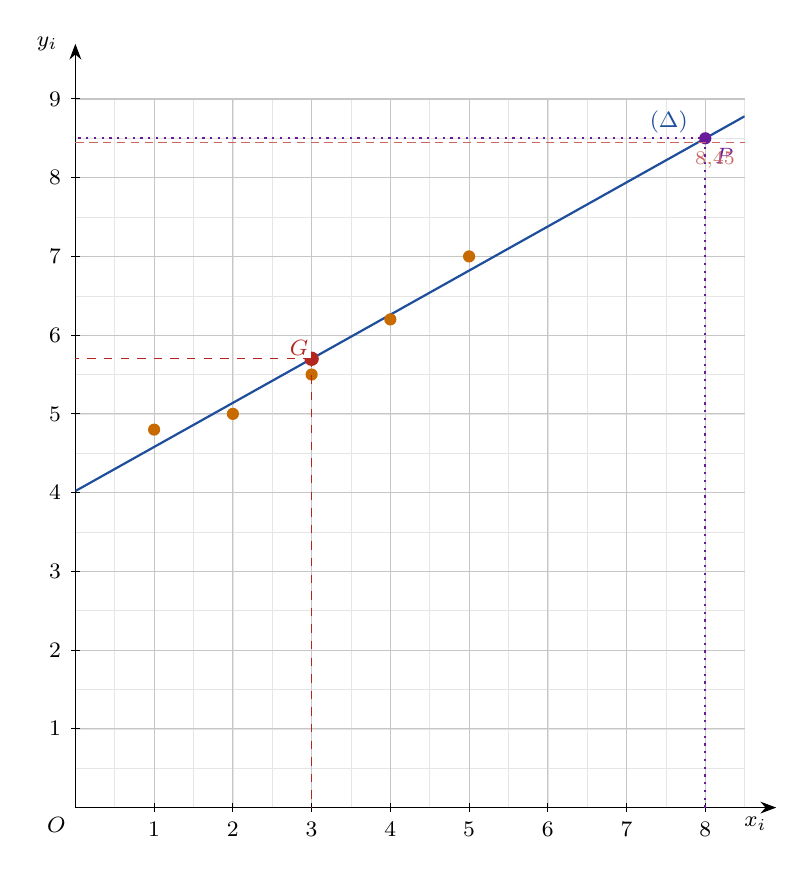
\begin{tikzpicture}[x=1cm,y=1cm,font=\footnotesize]
\draw[gray!20,very thin,step=0.5] (0,0) grid (8.500,9.000);
\draw[gray!45,thin,step=1] (0,0) grid (8.500,9.000);
\draw[-{Stealth[length=2mm]}] (0,0)--(8.900,0) node[below left]{$x_i$};
\draw[-{Stealth[length=2mm]}] (0,0)--(0,9.700) node[left=3pt]{$y_i$};
\node[below left] at (0,0){$O$};
\draw (1.000,0.06)--(1.000,-0.06) node[below]{$1$};
\draw (2.000,0.06)--(2.000,-0.06) node[below]{$2$};
\draw (3.000,0.06)--(3.000,-0.06) node[below]{$3$};
\draw (4.000,0.06)--(4.000,-0.06) node[below]{$4$};
\draw (5.000,0.06)--(5.000,-0.06) node[below]{$5$};
\draw (6.000,0.06)--(6.000,-0.06) node[below]{$6$};
\draw (7.000,0.06)--(7.000,-0.06) node[below]{$7$};
\draw (8.000,0.06)--(8.000,-0.06) node[below]{$8$};
\draw (0.06,1.000)--(-0.06,1.000) node[left]{$1$};
\draw (0.06,2.000)--(-0.06,2.000) node[left]{$2$};
\draw (0.06,3.000)--(-0.06,3.000) node[left]{$3$};
\draw (0.06,4.000)--(-0.06,4.000) node[left]{$4$};
\draw (0.06,5.000)--(-0.06,5.000) node[left]{$5$};
\draw (0.06,6.000)--(-0.06,6.000) node[left]{$6$};
\draw (0.06,7.000)--(-0.06,7.000) node[left]{$7$};
\draw (0.06,8.000)--(-0.06,8.000) node[left]{$8$};
\draw (0.06,9.000)--(-0.06,9.000) node[left]{$9$};
\begin{scope}\clip (0,0.000) rectangle (8.500,9.000);
\draw[cDef,thick,domain=0:8.500,samples=2] plot (\x*1.0000,{0.000000+(0.560000*\x+4.020000-0.000000)/1.000000});
\end{scope}
\node[cDef,above left] at (7.900,8.444){$(\Delta)$};
\fill[cEx] (1.000,4.800) circle (2.2pt);
\fill[cEx] (2.000,5.000) circle (2.2pt);
\fill[cEx] (3.000,5.500) circle (2.2pt);
\fill[cEx] (4.000,6.200) circle (2.2pt);
\fill[cEx] (5.000,7.000) circle (2.2pt);
\draw[cThm,dashed] (3.000,5.700)--(3.000,0) (3.000,5.700)--(0,5.700);
\fill[cThm] (3.000,5.700) circle (2.6pt) node[above left,fill=white,inner sep=1pt]{$G$};
\fill[cMeth] (8,8.5) circle (2.2pt) node[below right]{$P$};
\draw[cMeth,dotted,thick] (8,0)--(8,8.5)--(0,8.5);
\draw[cThm!70,densely dashed] (0,8.45)--(8.5,8.45) node[below left,font=\scriptsize]{$8{,}45$};
\end{tikzpicture}\end{LTR}\end{center}

\QQ{2} جدول الحسابات:
\begin{center}\small
\begin{tabular}{|C|c|c|c|c|c|C|}\hline
\rowcolor{cSec!12} $i$ & $1$ & $2$ & $3$ & $4$ & $5$ & المجموع\\\hline
$x_i$ & $1$ & $2$ & $3$ & $4$ & $5$ & $15$\\\hline
$y_i$ & $4{,}8$ & $5$ & $5{,}5$ & $6{,}2$ & $7$ & $28{,}5$\\\hline
$x_i^{2}$ & $1$ & $4$ & $9$ & $16$ & $25$ & $55$\\\hline
$x_iy_i$ & $4{,}8$ & $10$ & $16{,}5$ & $24{,}8$ & $35$ & $91{,}1$\\\hline
\end{tabular}
\end{center}
\textbf{التباين:}
\[V(x)=\frac1{5}\sum x_i^{2}-\bar x^{2}=\frac{55}{5}-3^{2}=2\]
\textbf{التغاير:}
\[\operatorname{cov}(x,y)=\frac1{5}\sum x_iy_i-\bar x\,\bar y=\frac{\sum x_iy_i-\bar x\sum y_i}{5}=\frac{91{,}1-3\times28{,}5}{5}=\frac{5{,}6}{5}=1{,}12\]

\[a=\frac{\operatorname{cov}(x,y)}{V(x)}=\frac{1{,}12}{2}=0{,}56\]
\[b=\bar y-a\bar x=5{,}7-0{,}56\times3=5{,}7-1{,}68=4{,}02\]
\[\bx{(\Delta):\ y=0{,}56\,x+4{,}02}\]
\QQ{3} سنة $2017$ رتبتها $x=2017-2009=8$:
\[y=0{,}56\times8+4{,}02=4{,}48+4{,}02=8{,}50\]
وبما أن $8{,}50>8{,}45$: \bxt{نعم، يمكن تحقيق الهدف حسب هذا التعديل (إنتاج متوقع $8{,}50$ مليون طن)}.
\QQ{4}
\[0{,}56\,x+4{,}02>10{,}17\iff 0{,}56\,x>6{,}15\iff x>\frac{6{,}15}{0{,}56}\approx10{,}98\]
أصغر رتبة صحيحة $x=11$، وهي سنة $2009+11=2020$: \bxt{يتعدى الإنتاج $10{,}17$ مليون طن ابتداءً من سنة $2020$} (تحقق: $0{,}56\times11+4{,}02=10{,}18>10{,}17$ و $0{,}56\times10+4{,}02=9{,}62$).
\end{hal}

% ===================== بكالوريا 2018 -- الموضوع الأول =====================
\Needspace{16\baselineskip}
\begin{tamrin}{بكالوريا 2018 -- الموضوع الأول -- تسيير واقتصاد}
يمثل الجدول التالي تطور النسب المئوية لنتائج شهادة البكالوريا في ثانوية ما، من سنة $2011$ إلى سنة $2017$.
\begin{center}
\begin{tabular}{|C|c|c|c|c|c|c|c|}\hline
\rowcolor{cSec!12} السنة & $2011$ & $2012$ & $2013$ & $2014$ & $2015$ & $2016$ & $2017$\\\hline
رتبة السنة $x_i$ & $1$ & $2$ & $3$ & $4$ & $5$ & $6$ & $7$\\\hline
النسبة المئوية $y_i$ & $44{,}78$ & $49{,}79$ & $51{,}36$ & $56{,}07$ & $58{,}84$ & $62{,}45$ & $75{,}01$\\\hline
\end{tabular}
\end{center}

\QQ{1} مثّل سحابة النقط $M_i(x_i;y_i)$ في معلم متعامد. (نأخذ $1\,\text{cm}$ لكل سنة على محور الفواصل و $1\,\text{cm}$ لكل $5\%$ على محور التراتيب)
\QQ{2} احسب $(\bar x;\bar y)$ إحداثيي $G$، النقطة المتوسطة لسحابة النقط $M_i(x_i;y_i)$.
\QQ{3} لتكن $y=ax+b$ معادلة مستقيم الانحدار بالمربعات الدنيا للسلسلة $(x_i;y_i)$. بيّن أن $a=4{,}41$ (تدوّر النتيجة إلى $10^{-2}$)، ثم احسب قيمة $b$.
\QQ{4} باستعمال التعديل الخطي السابق، ابتداءً من أي سنة تتجاوز نسبة النجاح $80\%$؟
\end{tamrin}
\Needspace{14cm}
\begin{hal}
\QQ{1} $1\,\text{cm}$ لكل سنة و $1\,\text{cm}$ لكل $5\%$. القيم بين $44{,}78$ و $75{,}01$، فنبدأ محور التراتيب من $40\%$ (المحور مقطوع قرب المبدأ) حتى لا يكون الشكل طويلا بلا فائدة؛ المستقيم $(\Delta)$ والنقطة $G$ من السؤالين 2 و 3:
\begin{center}\begin{LTR}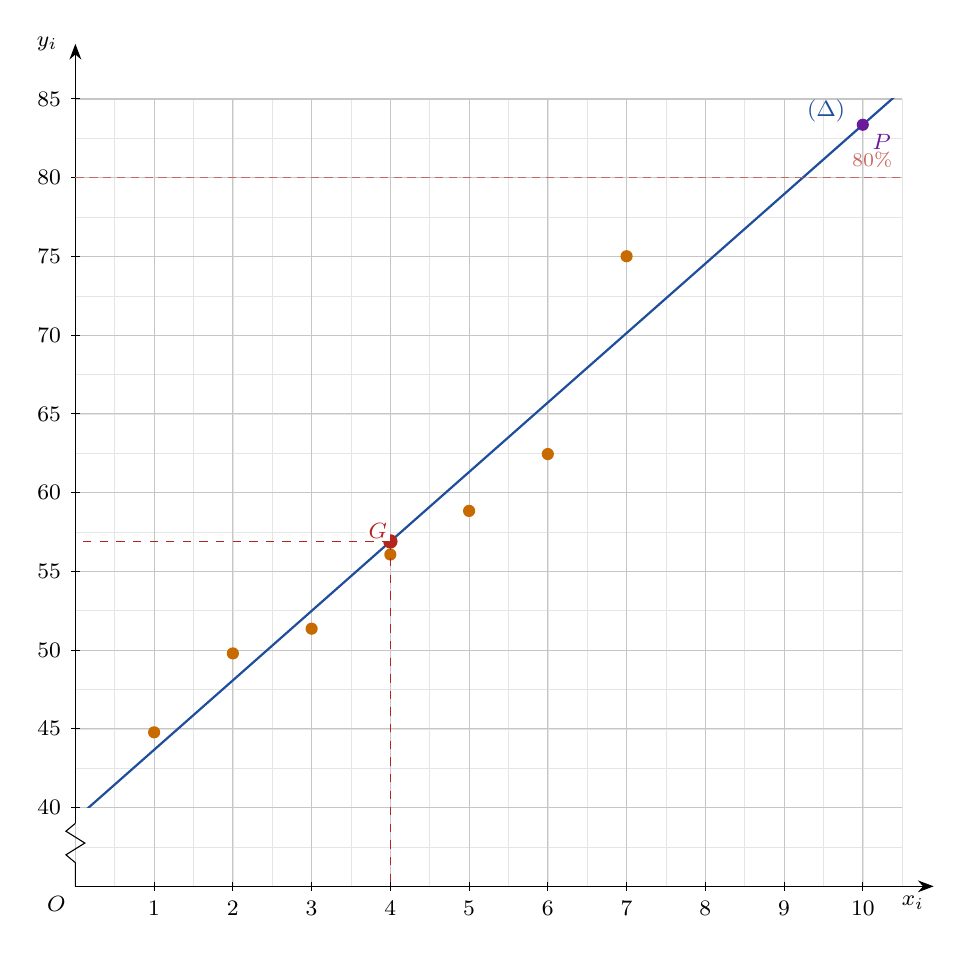
\begin{tikzpicture}[x=1cm,y=1cm,font=\footnotesize]
\draw[gray!20,very thin,step=0.5] (0,0) grid (10.500,10.000);
\draw[gray!45,thin,step=1] (0,0) grid (10.500,10.000);
\draw[-{Stealth[length=2mm]}] (0,0)--(10.900,0) node[below left]{$x_i$};
\draw (0,0)--(0,0.3)--(-0.12,0.4)--(0.12,0.55)--(-0.12,0.7)--(0,0.8);
\draw[-{Stealth[length=2mm]}] (0,0.8)--(0,10.700) node[left=3pt]{$y_i$};
\node[below left] at (0,0){$O$};
\draw (1.000,0.06)--(1.000,-0.06) node[below]{$1$};
\draw (2.000,0.06)--(2.000,-0.06) node[below]{$2$};
\draw (3.000,0.06)--(3.000,-0.06) node[below]{$3$};
\draw (4.000,0.06)--(4.000,-0.06) node[below]{$4$};
\draw (5.000,0.06)--(5.000,-0.06) node[below]{$5$};
\draw (6.000,0.06)--(6.000,-0.06) node[below]{$6$};
\draw (7.000,0.06)--(7.000,-0.06) node[below]{$7$};
\draw (8.000,0.06)--(8.000,-0.06) node[below]{$8$};
\draw (9.000,0.06)--(9.000,-0.06) node[below]{$9$};
\draw (10.000,0.06)--(10.000,-0.06) node[below]{$10$};
\draw (0.06,1.000)--(-0.06,1.000) node[left]{$40$};
\draw (0.06,2.000)--(-0.06,2.000) node[left]{$45$};
\draw (0.06,3.000)--(-0.06,3.000) node[left]{$50$};
\draw (0.06,4.000)--(-0.06,4.000) node[left]{$55$};
\draw (0.06,5.000)--(-0.06,5.000) node[left]{$60$};
\draw (0.06,6.000)--(-0.06,6.000) node[left]{$65$};
\draw (0.06,7.000)--(-0.06,7.000) node[left]{$70$};
\draw (0.06,8.000)--(-0.06,8.000) node[left]{$75$};
\draw (0.06,9.000)--(-0.06,9.000) node[left]{$80$};
\draw (0.06,10.000)--(-0.06,10.000) node[left]{$85$};
\begin{scope}\clip (0,1.000) rectangle (10.500,10.000);
\draw[cDef,thick,domain=0:10.500,samples=2] plot (\x*1.0000,{1.000000+(4.410000*\x+39.260000-40.000000)/5.000000});
\end{scope}
\node[cDef,above left] at (9.900,9.584){$(\Delta)$};
\fill[cEx] (1.000,1.956) circle (2.2pt);
\fill[cEx] (2.000,2.958) circle (2.2pt);
\fill[cEx] (3.000,3.272) circle (2.2pt);
\fill[cEx] (4.000,4.214) circle (2.2pt);
\fill[cEx] (5.000,4.768) circle (2.2pt);
\fill[cEx] (6.000,5.490) circle (2.2pt);
\fill[cEx] (7.000,8.002) circle (2.2pt);
\draw[cThm,dashed] (4.000,4.380)--(4.000,0) (4.000,4.380)--(0,4.380);
\fill[cThm] (4.000,4.380) circle (2.6pt) node[above left,fill=white,inner sep=1pt]{$G$};
\draw[cThm!70,densely dashed] (0,9)--(10.5,9) node[above left,font=\scriptsize]{$80\%$};
\fill[cMeth] (10,9.672) circle (2.2pt) node[below right]{$P$};
\end{tikzpicture}\end{LTR}\end{center}

\QQ{2}
\[\bar x=\dfrac{28}{7}=4\]
\[\bar y=\dfrac{44{,}78+49{,}79+51{,}36+56{,}07+58{,}84+62{,}45+75{,}01}{7}=\dfrac{398{,}3}{7}=56{,}9\]
\[\bx{G(4\,;\,56{,}9)}\]
\QQ{3} جدول الحسابات:
\begin{center}\small
\begin{tabular}{|C|c|c|c|c|c|c|c|C|}\hline
\rowcolor{cSec!12} $i$ & $1$ & $2$ & $3$ & $4$ & $5$ & $6$ & $7$ & المجموع\\\hline
$x_i$ & $1$ & $2$ & $3$ & $4$ & $5$ & $6$ & $7$ & $28$\\\hline
$y_i$ & $44{,}78$ & $49{,}79$ & $51{,}36$ & $56{,}07$ & $58{,}84$ & $62{,}45$ & $75{,}01$ & $398{,}3$\\\hline
$x_i^{2}$ & $1$ & $4$ & $9$ & $16$ & $25$ & $36$ & $49$ & $140$\\\hline
$x_iy_i$ & $44{,}78$ & $99{,}58$ & $154{,}08$ & $224{,}28$ & $294{,}2$ & $374{,}7$ & $525{,}07$ & $1716{,}69$\\\hline
\end{tabular}
\end{center}
\textbf{التباين:}
\[V(x)=\frac1{7}\sum x_i^{2}-\bar x^{2}=\frac{140}{7}-4^{2}=4\]
\textbf{التغاير:}
\[\operatorname{cov}(x,y)=\frac1{7}\sum x_iy_i-\bar x\,\bar y=\frac{\sum x_iy_i-\bar x\sum y_i}{7}=\frac{1716{,}69-4\times398{,}3}{7}=\frac{123{,}49}{7}\approx 17{,}6414\]

\[a=\frac{\operatorname{cov}(x,y)}{V(x)}=\frac{123{,}49/7}{4}=\frac{123{,}49}{28}\approx4{,}4104\approx4{,}41\]
\[b=\bar y-a\bar x=56{,}9-4{,}41\times4=56{,}9-17{,}64=39{,}26\]
\[\bx{y=4{,}41\,x+39{,}26}\]
\QQ{4}
\[4{,}41\,x+39{,}26>80\iff 4{,}41\,x>40{,}74\iff x>\frac{40{,}74}{4{,}41}\approx9{,}24\]
أصغر رتبة صحيحة $x=10$، وهي سنة $2010+10=2020$ (تحقق: $x=9$ يعطي $78{,}95$، و $x=10$ يعطي $83{,}36$).
\bxt{تتجاوز نسبة النجاح $80\%$ ابتداءً من سنة $2020$} (النقطة $P$ على الشكل).
\end{hal}

% ===================== بكالوريا 2018 -- الموضوع الثاني =====================
\Needspace{16\baselineskip}
\begin{tamrin}{بكالوريا 2018 -- الموضوع الثاني -- تسيير واقتصاد}
الجدول التالي يمثل تطور عدد المتقاعدين من سنة $2009$ إلى سنة $2014$ بالجزائر. (الديوان الوطني للإحصائيات)
\begin{center}
\begin{tabular}{|C|c|c|c|c|c|c|}\hline
\rowcolor{cSec!12} السنة & $2010$ & $2011$ & $2012$ & $2013$ & $2014$ & $2015$\\\hline
رتبة السنة $x_i$ & $1$ & $2$ & $3$ & $4$ & $5$ & $6$\\\hline
عدد المتقاعدين $y_i$ (بالملايين) & $2{,}17$ & $2{,}19$ & $2{,}32$ & $2{,}48$ & $2{,}63$ & $2{,}77$\\\hline
\end{tabular}
\end{center}

\QQ{1} مثّل سحابة النقط $M_i(x_i;y_i)$ في معلم متعامد. (نأخذ كوحدة بيانية: $2\,\text{cm}$ لكل سنة على محور الفواصل و $2\,\text{cm}$ لكل مليون متقاعد على محور التراتيب)
\QQ{2} عيّن إحداثيي النقطة المتوسطة $G$ ثم علّمها.
\QQ{3} اكتب معادلة مستقيم الانحدار بالمربعات الدنيا.
\QQ{4} نفرض أن تطور عدد المتقاعدين يبقى على هذه الوتيرة في السنوات الموالية.
\begin{itemize}
\item قدّر عدد المتقاعدين في الجزائر سنة $2020$.
\item ابتداءً من أي سنة يتعدى عدد المتقاعدين في الجزائر $4$ ملايين؟
\end{itemize}
\end{tamrin}
\begin{molahada}
النص يذكر الفترة «من $2009$ إلى $2014$» بينما سنوات الجدول من $2010$ إلى $2015$. نعتمد الجدول: الرتبة $x$ توافق السنة $2009+x$.
\end{molahada}
\Needspace{10.5cm}
\begin{hal}
\QQ{1} $2\,\text{cm}$ لكل سنة و $2\,\text{cm}$ لكل مليون (أي $1\,\text{cm}$ لكل $0{,}5$ مليون)، فالنقطة $M_i$ على الورقة هي $(2x_i\,;\,2y_i)$ بالسنتيمتر:
\begin{center}\begin{LTR}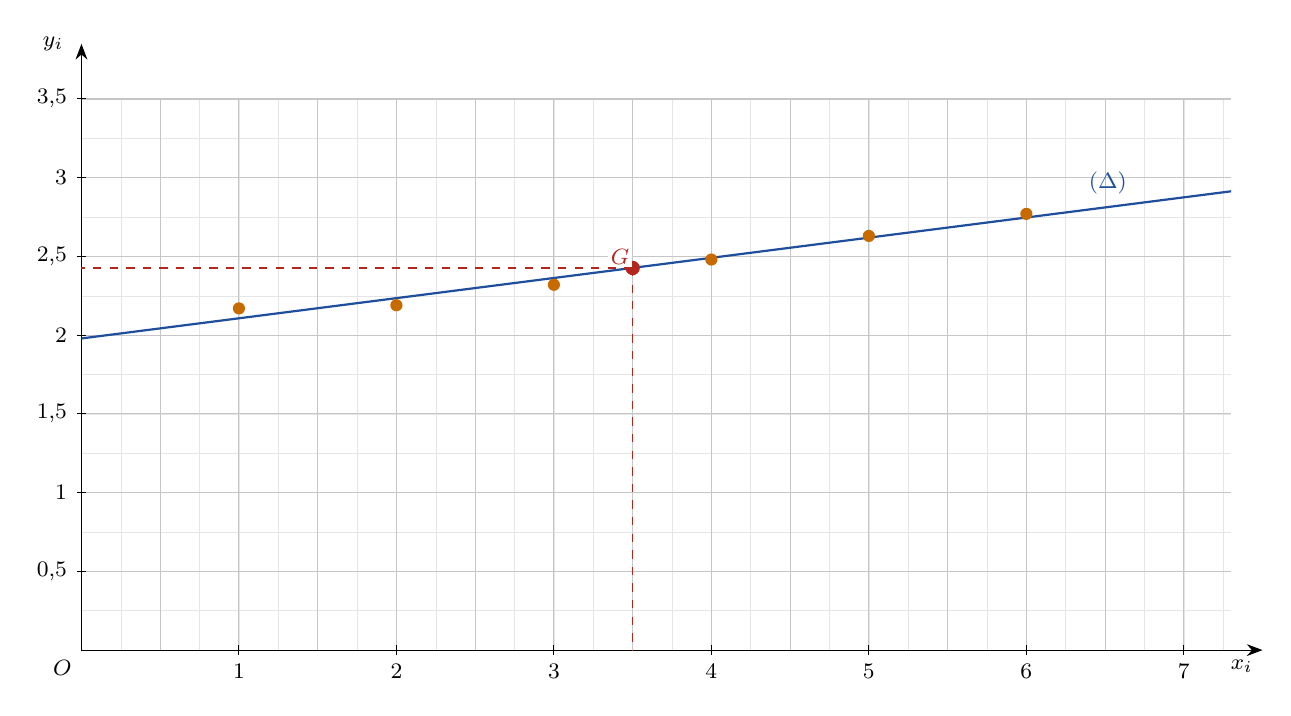
\begin{tikzpicture}[x=1cm,y=1cm,font=\footnotesize]
\draw[gray!20,very thin,step=0.5] (0,0) grid (14.600,7.000);
\draw[gray!45,thin,step=1] (0,0) grid (14.600,7.000);
\draw[-{Stealth[length=2mm]}] (0,0)--(15.000,0) node[below left]{$x_i$};
\draw[-{Stealth[length=2mm]}] (0,0)--(0,7.700) node[left=3pt]{$y_i$};
\node[below left] at (0,0){$O$};
\draw (2.000,0.06)--(2.000,-0.06) node[below]{$1$};
\draw (4.000,0.06)--(4.000,-0.06) node[below]{$2$};
\draw (6.000,0.06)--(6.000,-0.06) node[below]{$3$};
\draw (8.000,0.06)--(8.000,-0.06) node[below]{$4$};
\draw (10.000,0.06)--(10.000,-0.06) node[below]{$5$};
\draw (12.000,0.06)--(12.000,-0.06) node[below]{$6$};
\draw (14.000,0.06)--(14.000,-0.06) node[below]{$7$};
\draw (0.06,1.000)--(-0.06,1.000) node[left]{$0{,}5$};
\draw (0.06,2.000)--(-0.06,2.000) node[left]{$1$};
\draw (0.06,3.000)--(-0.06,3.000) node[left]{$1{,}5$};
\draw (0.06,4.000)--(-0.06,4.000) node[left]{$2$};
\draw (0.06,5.000)--(-0.06,5.000) node[left]{$2{,}5$};
\draw (0.06,6.000)--(-0.06,6.000) node[left]{$3$};
\draw (0.06,7.000)--(-0.06,7.000) node[left]{$3{,}5$};
\begin{scope}\clip (0,0.000) rectangle (14.600,7.000);
\draw[cDef,thick,domain=0:7.300,samples=2] plot (\x*2.0000,{0.000000+(0.128000*\x+1.979000-0.000000)/0.500000});
\end{scope}
\node[cDef,above left] at (13.400,5.673){$(\Delta)$};
\fill[cEx] (2.000,4.340) circle (2.2pt);
\fill[cEx] (4.000,4.380) circle (2.2pt);
\fill[cEx] (6.000,4.640) circle (2.2pt);
\fill[cEx] (8.000,4.960) circle (2.2pt);
\fill[cEx] (10.000,5.260) circle (2.2pt);
\fill[cEx] (12.000,5.540) circle (2.2pt);
\draw[cThm,dashed] (7.000,4.853)--(7.000,0) (7.000,4.853)--(0,4.853);
\fill[cThm] (7.000,4.853) circle (2.6pt) node[above left,fill=white,inner sep=1pt]{$G$};
\end{tikzpicture}\end{LTR}\end{center}

\QQ{2}
\[\bar x=\dfrac{21}{6}=3{,}5\]
\[\bar y=\dfrac{2{,}17+2{,}19+2{,}32+2{,}48+2{,}63+2{,}77}{6}=\dfrac{14{,}56}{6}\approx2{,}427\]
\[\bx{G(3{,}5\,;\,2{,}427)}\quad(\text{تقريبا } G(3{,}5\,;\,2{,}43))\]
\QQ{3} جدول الحسابات:
\begin{center}\small
\begin{tabular}{|C|c|c|c|c|c|c|C|}\hline
\rowcolor{cSec!12} $i$ & $1$ & $2$ & $3$ & $4$ & $5$ & $6$ & المجموع\\\hline
$x_i$ & $1$ & $2$ & $3$ & $4$ & $5$ & $6$ & $21$\\\hline
$y_i$ & $2{,}17$ & $2{,}19$ & $2{,}32$ & $2{,}48$ & $2{,}63$ & $2{,}77$ & $14{,}56$\\\hline
$x_i^{2}$ & $1$ & $4$ & $9$ & $16$ & $25$ & $36$ & $91$\\\hline
$x_iy_i$ & $2{,}17$ & $4{,}38$ & $6{,}96$ & $9{,}92$ & $13{,}15$ & $16{,}62$ & $53{,}2$\\\hline
\end{tabular}
\end{center}
\textbf{التباين:}
\[V(x)=\frac1{6}\sum x_i^{2}-\bar x^{2}=\frac{91}{6}-(3{,}5)^{2}=\frac{35}{12}\approx 2{,}9167\]
\textbf{التغاير:}
\[\operatorname{cov}(x,y)=\frac1{6}\sum x_iy_i-\bar x\,\bar y=\frac{\sum x_iy_i-\bar x\sum y_i}{6}=\frac{53{,}2-3{,}5\times14{,}56}{6}=\frac{2{,}24}{6}\approx 0{,}3733\]

\[a=\frac{\operatorname{cov}(x,y)}{V(x)}=\frac{2{,}24/6}{35/12}=\frac{2{,}24\times2}{35}=0{,}128\]
\[b=\bar y-a\bar x=\frac{14{,}56}{6}-0{,}128\times3{,}5\approx2{,}4267-0{,}448=1{,}9787\]
\[\bx{y=0{,}128\,x+1{,}979}\]
(بالتدوير إلى $10^{-2}$: $y=0{,}13x+1{,}98$.) $(\Delta)$ يشمل $G$ و $(0\,;1{,}979)$.
\QQ{4}
\begin{itemize}
\item سنة $2020$ رتبتها $x=2020-2009=11$:
\[y=0{,}128\times11+1{,}979=1{,}408+1{,}979=3{,}387\]
\bxt{عدد المتقاعدين المقدّر سنة $2020$: حوالي $3{,}39$ مليون متقاعد} (بالمعادلة المدوّرة إلى $10^{-2}$ نجد $3{,}41$ مليون).
\item نحل المتراجحة $y>4$:
\[0{,}128\,x+1{,}979>4\iff 0{,}128\,x>2{,}021\iff x>\frac{2{,}021}{0{,}128}\approx15{,}79\]
فأصغر رتبة صحيحة $x=16$، وهي سنة $2009+16=2025$ (وبالمعادلة المدوّرة: $0{,}13x+1{,}98>4\iff x>15{,}54$، نفس النتيجة).
\bxt{يتعدى عدد المتقاعدين $4$ ملايين ابتداءً من سنة $2025$}.
\end{itemize}
\end{hal}

% ===================== بكالوريا 2019 -- الموضوع الأول =====================
\Needspace{16\baselineskip}
\begin{tamrin}{بكالوريا 2019 -- الموضوع الأول -- تسيير واقتصاد}
يمثل الجدول التالي تطور الواردات في الجزائر مقدّرة بالمليار دولار من سنة $2009$ إلى سنة $2014$.
\begin{center}
\begin{tabular}{|C|c|c|c|c|c|c|}\hline
\rowcolor{cSec!12} السنة & $2009$ & $2010$ & $2011$ & $2012$ & $2013$ & $2014$\\\hline
رتبة السنة $x_i$ & $1$ & $2$ & $3$ & $4$ & $5$ & $6$\\\hline
الواردات $y_i$ & $39{,}29$ & $40{,}47$ & $47{,}25$ & $47{,}49$ & $54{,}85$ & $58{,}33$\\\hline
\end{tabular}
\end{center}

\QQ{1} مثّل سحابة النقط $M_i(x_i;y_i)$ في معلم متعامد. (نأخذ $1\,\text{cm}$ لكل سنة على محور الفواصل و $1\,\text{cm}$ لكل $10$ مليار دولار على محور التراتيب)
\QQ{2} جد إحداثيي النقطة المتوسطة $G$، ثم علّمها.
\QQ{3} بيّن أن معادلة مستقيم الانحدار $(\Delta)$ بالمربعات الدنيا لهذه السلسلة الإحصائية هي: $y=3{,}96x+34{,}09$، ثم مثّل $(\Delta)$.
\QQ{4} اعتمادًا على التعديل الخطي السابق، ابتداءً من أي سنة تفوق الواردات $77$ مليار دولار؟
\end{tamrin}
\Needspace{12.5cm}
\begin{hal}
\QQ{1} $1\,\text{cm}$ لكل سنة و $1\,\text{cm}$ لكل $10$ مليار دولار (ترتيب $M_i$ على الورقة $\frac{y_i}{10}$ cm):
\begin{center}\begin{LTR}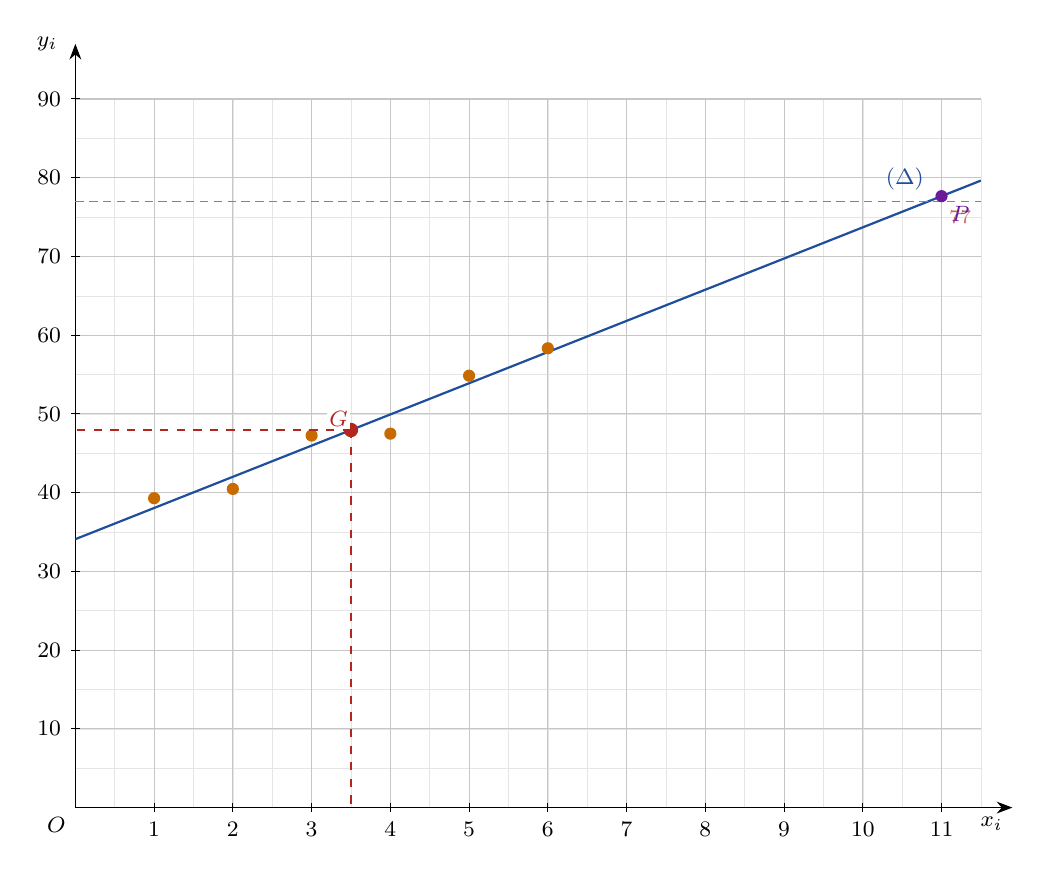
\begin{tikzpicture}[x=1cm,y=1cm,font=\footnotesize]
\draw[gray!20,very thin,step=0.5] (0,0) grid (11.500,9.000);
\draw[gray!45,thin,step=1] (0,0) grid (11.500,9.000);
\draw[-{Stealth[length=2mm]}] (0,0)--(11.900,0) node[below left]{$x_i$};
\draw[-{Stealth[length=2mm]}] (0,0)--(0,9.700) node[left=3pt]{$y_i$};
\node[below left] at (0,0){$O$};
\draw (1.000,0.06)--(1.000,-0.06) node[below]{$1$};
\draw (2.000,0.06)--(2.000,-0.06) node[below]{$2$};
\draw (3.000,0.06)--(3.000,-0.06) node[below]{$3$};
\draw (4.000,0.06)--(4.000,-0.06) node[below]{$4$};
\draw (5.000,0.06)--(5.000,-0.06) node[below]{$5$};
\draw (6.000,0.06)--(6.000,-0.06) node[below]{$6$};
\draw (7.000,0.06)--(7.000,-0.06) node[below]{$7$};
\draw (8.000,0.06)--(8.000,-0.06) node[below]{$8$};
\draw (9.000,0.06)--(9.000,-0.06) node[below]{$9$};
\draw (10.000,0.06)--(10.000,-0.06) node[below]{$10$};
\draw (11.000,0.06)--(11.000,-0.06) node[below]{$11$};
\draw (0.06,1.000)--(-0.06,1.000) node[left]{$10$};
\draw (0.06,2.000)--(-0.06,2.000) node[left]{$20$};
\draw (0.06,3.000)--(-0.06,3.000) node[left]{$30$};
\draw (0.06,4.000)--(-0.06,4.000) node[left]{$40$};
\draw (0.06,5.000)--(-0.06,5.000) node[left]{$50$};
\draw (0.06,6.000)--(-0.06,6.000) node[left]{$60$};
\draw (0.06,7.000)--(-0.06,7.000) node[left]{$70$};
\draw (0.06,8.000)--(-0.06,8.000) node[left]{$80$};
\draw (0.06,9.000)--(-0.06,9.000) node[left]{$90$};
\begin{scope}\clip (0,0.000) rectangle (11.500,9.000);
\draw[cDef,thick,domain=0:11.500,samples=2] plot (\x*1.0000,{0.000000+(3.960000*\x+34.090000-0.000000)/10.000000});
\end{scope}
\node[cDef,above left] at (10.900,7.725){$(\Delta)$};
\fill[cEx] (1.000,3.929) circle (2.2pt);
\fill[cEx] (2.000,4.047) circle (2.2pt);
\fill[cEx] (3.000,4.725) circle (2.2pt);
\fill[cEx] (4.000,4.749) circle (2.2pt);
\fill[cEx] (5.000,5.485) circle (2.2pt);
\fill[cEx] (6.000,5.833) circle (2.2pt);
\draw[cThm,dashed] (3.500,4.795)--(3.500,0) (3.500,4.795)--(0,4.795);
\fill[cThm] (3.500,4.795) circle (2.6pt) node[above left,fill=white,inner sep=1pt]{$G$};
\draw[cThm!70,densely dashed] (0,7.7)--(11.5,7.7) node[below left,font=\scriptsize]{$77$};
\fill[cMeth] (11,7.765) circle (2.2pt) node[below right]{$P$};
\end{tikzpicture}\end{LTR}\end{center}

\QQ{2}
\[\bar x=\dfrac{21}{6}=3{,}5\]
\[\bar y=\dfrac{39{,}29+40{,}47+47{,}25+47{,}49+54{,}85+58{,}33}{6}=\dfrac{287{,}68}{6}\approx47{,}95\]
\[\bx{G(3{,}5\,;\,47{,}95)}\]
\QQ{3} جدول الحسابات:
\begin{center}\small
\begin{tabular}{|C|c|c|c|c|c|c|C|}\hline
\rowcolor{cSec!12} $i$ & $1$ & $2$ & $3$ & $4$ & $5$ & $6$ & المجموع\\\hline
$x_i$ & $1$ & $2$ & $3$ & $4$ & $5$ & $6$ & $21$\\\hline
$y_i$ & $39{,}29$ & $40{,}47$ & $47{,}25$ & $47{,}49$ & $54{,}85$ & $58{,}33$ & $287{,}68$\\\hline
$x_i^{2}$ & $1$ & $4$ & $9$ & $16$ & $25$ & $36$ & $91$\\\hline
$x_iy_i$ & $39{,}29$ & $80{,}94$ & $141{,}75$ & $189{,}96$ & $274{,}25$ & $349{,}98$ & $1076{,}17$\\\hline
\end{tabular}
\end{center}
\textbf{التباين:}
\[V(x)=\frac1{6}\sum x_i^{2}-\bar x^{2}=\frac{91}{6}-(3{,}5)^{2}=\frac{35}{12}\approx 2{,}9167\]
\textbf{التغاير:}
\[\operatorname{cov}(x,y)=\frac1{6}\sum x_iy_i-\bar x\,\bar y=\frac{\sum x_iy_i-\bar x\sum y_i}{6}=\frac{1076{,}17-3{,}5\times287{,}68}{6}=\frac{69{,}29}{6}\approx 11{,}5483\]

\[a=\frac{\operatorname{cov}(x,y)}{V(x)}=\frac{69{,}29/6}{35/12}=\frac{69{,}29\times2}{35}\approx3{,}9594\approx3{,}96\]
\[b=\bar y-a\bar x\approx47{,}9467-3{,}9594\times3{,}5\approx47{,}9467-13{,}8580=34{,}0887\approx34{,}09\]
\[\bx{(\Delta):\ y=3{,}96\,x+34{,}09}\]
وهي المعادلة المطلوبة. لتمثيله: يشمل $G(3{,}5;47{,}95)$ و $(0;34{,}09)$.
\QQ{4}
\[3{,}96\,x+34{,}09>77\iff 3{,}96\,x>42{,}91\iff x>\frac{42{,}91}{3{,}96}\approx10{,}84\]
أصغر رتبة صحيحة $x=11$، وهي سنة $2008+11=2019$ (تحقق: $x=10$ يعطي $73{,}69$، و $x=11$ يعطي $77{,}65$).
\bxt{تفوق الواردات $77$ مليار دولار ابتداءً من سنة $2019$}.
\end{hal}

% ===================== بكالوريا 2019 -- الموضوع الثاني =====================
\Needspace{16\baselineskip}
\begin{tamrin}{بكالوريا 2019 -- الموضوع الثاني -- تسيير واقتصاد}
يمثل الجدول التالي تطور الإنتاج السنوي (الوحدة: الطن) لأحد أنواع الأسماك في حوض مائي لتربية الأسماك.
\begin{center}
\begin{tabular}{|C|c|c|c|c|c|c|}\hline
\rowcolor{cSec!12} السنة & $2013$ & $2014$ & $2015$ & $2016$ & $2017$ & $2018$\\\hline
رتبة السنة $x_i$ & $1$ & $2$ & $3$ & $4$ & $5$ & $6$\\\hline
الواردات $y_i$ & $490$ & $510$ & $595$ & $630$ & $840$ & $999$\\\hline
\end{tabular}
\end{center}

\QQ{1} مثّل سحابة النقط $M_i(x_i;y_i)$ في معلم متعامد. (نأخذ $1\,\text{cm}$ لكل سنة على محور الفواصل و $1\,\text{cm}$ لكل $100$ طن على محور التراتيب)
\QQ{2} جد إحداثيي النقطة المتوسطة $G$ لهذه السحابة.
\QQ{3} بيّن أن معادلة لمستقيم الانحدار بالمربعات الدنيا لهذه السلسلة الإحصائية هي: $y=102x+320{,}33$، ومثّله بيانيًا.
\QQ{4} باعتبار أن كمية الإنتاج تتبع نفس الوتيرة:
\begin{sq}
\qa ما هي كمية الإنتاج المتوقعة سنة $2023$؟
\qb ابتداءً من أي سنة تتجاوز كمية الإنتاج $2000$ طن؟
\end{sq}
\end{tamrin}
\begin{molahada}
السطر الثالث من الجدول عنوانه «الواردات» وهو خطأ في النص: المقصود \textbf{كمية الإنتاج $y_i$ بالطن}، كما يدل عليه نص التمرين والأسئلة.
\end{molahada}
\Needspace{14.5cm}
\begin{hal}
\QQ{1} $1\,\text{cm}$ لكل سنة و $1\,\text{cm}$ لكل $100$ طن (ترتيب $M_i$ على الورقة $\frac{y_i}{100}$ cm):
\begin{center}\begin{LTR}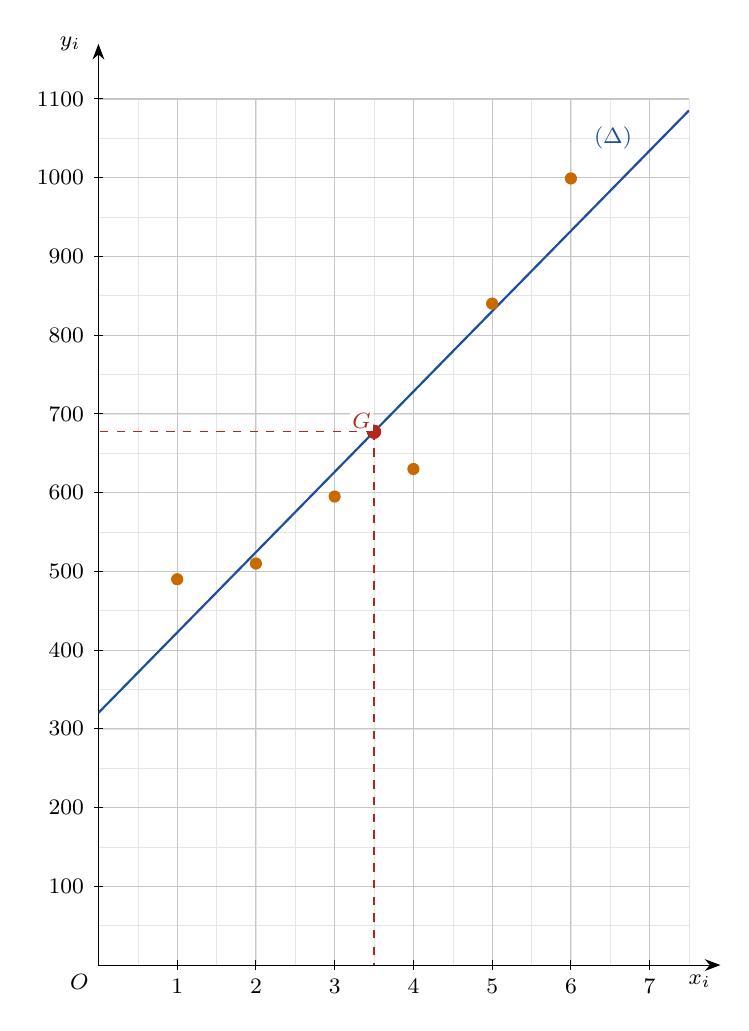
\begin{tikzpicture}[x=1cm,y=1cm,font=\footnotesize]
\draw[gray!20,very thin,step=0.5] (0,0) grid (7.500,11.000);
\draw[gray!45,thin,step=1] (0,0) grid (7.500,11.000);
\draw[-{Stealth[length=2mm]}] (0,0)--(7.900,0) node[below left]{$x_i$};
\draw[-{Stealth[length=2mm]}] (0,0)--(0,11.700) node[left=3pt]{$y_i$};
\node[below left] at (0,0){$O$};
\draw (1.000,0.06)--(1.000,-0.06) node[below]{$1$};
\draw (2.000,0.06)--(2.000,-0.06) node[below]{$2$};
\draw (3.000,0.06)--(3.000,-0.06) node[below]{$3$};
\draw (4.000,0.06)--(4.000,-0.06) node[below]{$4$};
\draw (5.000,0.06)--(5.000,-0.06) node[below]{$5$};
\draw (6.000,0.06)--(6.000,-0.06) node[below]{$6$};
\draw (7.000,0.06)--(7.000,-0.06) node[below]{$7$};
\draw (0.06,1.000)--(-0.06,1.000) node[left]{$100$};
\draw (0.06,2.000)--(-0.06,2.000) node[left]{$200$};
\draw (0.06,3.000)--(-0.06,3.000) node[left]{$300$};
\draw (0.06,4.000)--(-0.06,4.000) node[left]{$400$};
\draw (0.06,5.000)--(-0.06,5.000) node[left]{$500$};
\draw (0.06,6.000)--(-0.06,6.000) node[left]{$600$};
\draw (0.06,7.000)--(-0.06,7.000) node[left]{$700$};
\draw (0.06,8.000)--(-0.06,8.000) node[left]{$800$};
\draw (0.06,9.000)--(-0.06,9.000) node[left]{$900$};
\draw (0.06,10.000)--(-0.06,10.000) node[left]{$1000$};
\draw (0.06,11.000)--(-0.06,11.000) node[left]{$1100$};
\begin{scope}\clip (0,0.000) rectangle (7.500,11.000);
\draw[cDef,thick,domain=0:7.500,samples=2] plot (\x*1.0000,{0.000000+(102.000000*\x+320.330000-0.000000)/100.000000});
\end{scope}
\node[cDef,above left] at (6.900,10.241){$(\Delta)$};
\fill[cEx] (1.000,4.900) circle (2.2pt);
\fill[cEx] (2.000,5.100) circle (2.2pt);
\fill[cEx] (3.000,5.950) circle (2.2pt);
\fill[cEx] (4.000,6.300) circle (2.2pt);
\fill[cEx] (5.000,8.400) circle (2.2pt);
\fill[cEx] (6.000,9.990) circle (2.2pt);
\draw[cThm,dashed] (3.500,6.773)--(3.500,0) (3.500,6.773)--(0,6.773);
\fill[cThm] (3.500,6.773) circle (2.6pt) node[above left,fill=white,inner sep=1pt]{$G$};
\end{tikzpicture}\end{LTR}\end{center}

\QQ{2}
\[\bar x=\dfrac{21}{6}=3{,}5\]
\[\bar y=\dfrac{490+510+595+630+840+999}{6}=\dfrac{4064}{6}\approx677{,}33\]
\[\bx{G(3{,}5\,;\,677{,}33)}\]
\QQ{3} جدول الحسابات:
\begin{center}\small
\begin{tabular}{|C|c|c|c|c|c|c|C|}\hline
\rowcolor{cSec!12} $i$ & $1$ & $2$ & $3$ & $4$ & $5$ & $6$ & المجموع\\\hline
$x_i$ & $1$ & $2$ & $3$ & $4$ & $5$ & $6$ & $21$\\\hline
$y_i$ & $490$ & $510$ & $595$ & $630$ & $840$ & $999$ & $4064$\\\hline
$x_i^{2}$ & $1$ & $4$ & $9$ & $16$ & $25$ & $36$ & $91$\\\hline
$x_iy_i$ & $490$ & $1020$ & $1785$ & $2520$ & $4200$ & $5994$ & $16009$\\\hline
\end{tabular}
\end{center}
\textbf{التباين:}
\[V(x)=\frac1{6}\sum x_i^{2}-\bar x^{2}=\frac{91}{6}-(3{,}5)^{2}=\frac{35}{12}\approx 2{,}9167\]
\textbf{التغاير:}
\[\operatorname{cov}(x,y)=\frac1{6}\sum x_iy_i-\bar x\,\bar y=\frac{\sum x_iy_i-\bar x\sum y_i}{6}=\frac{16009-3{,}5\times4064}{6}=\frac{1785}{6}=297{,}5\]

\[a=\frac{\operatorname{cov}(x,y)}{V(x)}=\frac{1785/6}{35/12}=\frac{1785\times2}{35}=102\]
\[b=\bar y-a\bar x=\frac{4064}{6}-102\times3{,}5=677{,}33-357=320{,}33\]
\[\bx{y=102\,x+320{,}33}\]
وهي المعادلة المطلوبة. لتمثيله: يشمل $G(3{,}5;677{,}33)$ و $(0;320{,}33)$ (أو $(6;932{,}33)$).
\QQ{4}
\pa سنة $2023$ رتبتها $x=2023-2012=11$:
\[y=102\times11+320{,}33=1122+320{,}33=1442{,}33\]
\bxt{كمية الإنتاج المتوقعة سنة $2023$: حوالي $1442{,}33$ طن}.
\pb
\[102\,x+320{,}33>2000\iff 102\,x>1679{,}67\iff x>\frac{1679{,}67}{102}\approx16{,}47\]
أصغر رتبة صحيحة $x=17$، وهي سنة $2012+17=2029$ (تحقق: $x=16$ يعطي $1952{,}33$، و $x=17$ يعطي $2054{,}33$).
\bxt{تتجاوز كمية الإنتاج $2000$ طن ابتداءً من سنة $2029$}.
\end{hal}
\end{document}
